%%%%%%%%%%%%%%%%%%%%%%%%%%%%%%%%%%%%%%%%%%%%%%%%%%%%%%%%%%%%%%%%%%%%%%%%%%%%%%%
%
%  Introduction to Cast3M programming
%  Andrei Constantinescu -- LMS, CNRS UMR 7649, Ecole Polytechnique
%
%  Build:   latexmk -pdf castem        (runs pdflatex/bibtex/makeindex as needed)
%  or:      pdflatex castem ; bibtex castem ; makeindex castem ; pdflatex castem
%
%  ---------------------------------------------------------------------------
%  ENCODING.  All .tex sources in this directory are UTF-8.  They used to be
%  a mixture of latin-1 and ASCII, which is what produced the mojibake
%  ("é" for "é") and the "Unicode character not set up for use with LaTeX"
%  errors.  If you edit a file, keep it UTF-8.  To check:
%      file *.tex                    (should say "UTF-8 text" everywhere)
%  To convert a stray latin-1 file:
%      iconv -f ISO-8859-1 -t UTF-8 file.tex -o file.tex.new && mv ...
%  ---------------------------------------------------------------------------
%
%%%%%%%%%%%%%%%%%%%%%%%%%%%%%%%%%%%%%%%%%%%%%%%%%%%%%%%%%%%%%%%%%%%%%%%%%%%%%%%

\documentclass[english,11pt]{book}

\usepackage[T1]{fontenc}
\usepackage[utf8]{inputenc}
% "english" is also a global option on \documentclass, so the main language
% has to be named explicitly -- otherwise babel takes the last one it
% processes (french) and you get French spacing and em-dash lists in an
% English book.  Use \begin{otherlanguage}{french} ... for French passages.
\usepackage[main=english,french]{babel}
\usepackage{graphicx,verbatim}
\usepackage{xcolor}
\usepackage{amsmath,amssymb}
\usepackage{makeidx,placeins}
\usepackage{array}
\usepackage{enumitem}
\usepackage[expansion=false]{microtype}   % cmtt is a bitmap font here, so
                                         % font expansion has to stay off

\usepackage{mathptmx}                % Times text + matching maths
                                     % (replaces the obsolete "times" package,
                                     %  which left the maths in Computer Modern)
\usepackage[scaled=0.92]{helvet}     % Helvetica for the sans family, i.e. for
                                     % the headings below -- \sffamily is used
                                     % nowhere else in the document.  Helvetica
                                     % runs large next to Times, hence the
                                     % 0.92 scaling.

\usepackage[colorlinks=true,linkcolor=linknavy,citecolor=linknavy,
            urlcolor=linknavy,breaklinks=true]{hyperref}
\usepackage{url}
\usepackage{xurl}        % lets long query-string URLs break anywhere

\setlength{\topmargin}{-10.mm}
\setlength{\textwidth}{170.mm}
\setlength{\textheight}{220.mm}
\setlength{\parindent}{0.5cm}
\setlength{\oddsidemargin}{0.cm}
\setlength{\evensidemargin}{0.cm}

\setlength{\emergencystretch}{3em}   % keeps long paths/URLs inside the margin
\Urlmuskip=0mu plus 1mu\relax

\renewcommand{\ttdefault}{cmtt}


\newcommand{\bfm}[1]{\mbox{\boldmath $#1$}}
\newcommand{\tr}{\mbox{\rm{tr}}}
\newcommand{\dev}{\mbox{\rm{dev}}}
\DeclareMathOperator*{\argmin}{arg\;min}

\newcommand{\derp}[2]{\frac{\partial #1}{\partial #2}}

\newcommand{\vect}[1]{\underline{#1}}
\newcommand{\tens}[1]{\underline{\underline{{#1}}}}
\newcommand{\tenq}[1]{\pmb{#1}}

\newcommand{\grad}{\text{grad}\,}
\newcommand{\ddiv}{\text{div}\,}
\newcommand{\mexp}{\text{exp}\,}

\newcommand{\bcddot}{\, \bfm{:} \,}
\newcommand{\bcdot}{\, \bfm{\cdot} \,}

\newcommand{\jump}[1]{\lbrack\!\lbrack #1 \rbrack\!\rbrack}
\newcommand{\norm}[1]{|\!| #1 |\!|}
\newcommand{\abs}[1]{| #1 |}
\newcommand{\func}[1]{\mbox{\rm #1}}

%%%%%%%%%%%%%%%%%%%%%%%%%%%%%%%%%%%%%%%%%%%%%%%%%%%%%%%%%%%%%%%%%%%%%%%%%%%%%%%
%  Index macros
%
%  The index is a double-entry index: each gibiane operator is listed under
%  its own name followed by its english meaning, and again under the english
%  meaning followed by the operator.
%
%     \dindex{cerc[le]}{circle}  ->  cerc[le] (circle), 12
%                                    circle cerc[le], 12
%     \sindex{pasapas}           ->  pasapas, 34
%
%  The sort keys ("#1 #2d@...") keep the operator entries next to each other.
%  Note: the braces in \index{...} must be balanced, and a bare "[" is fine
%  but a "!" or "@" inside the visible text has to be escaped with ".
%%%%%%%%%%%%%%%%%%%%%%%%%%%%%%%%%%%%%%%%%%%%%%%%%%%%%%%%%%%%%%%%%%%%%%%%%%%%%%%

\newcommand{\dindex}[2]{%
\index{#1 #2d@\texttt{#1} (#2)}%
\index{#2 #1@#2 \texttt{#1}}%
}

\newcommand{\sindex}[1]{%
\index{#1d@\texttt{#1}}%
}

% \cindex{...} indexes a CONCEPT rather than an operator, in roman type.
%  \dindex and \sindex both typeset their entry in \texttt, which is right for
%  an operator name and wrong for "imperfection sensitivity".  Same sorting
%  convention as the others, so the three interleave correctly.
%     \cindex{buckling}                        -> buckling, 43
%     \cindex[theta-method]{$\theta$-method}   -> sorts as "theta-method"
%  The optional argument is the sort key, needed whenever the visible text
%  starts with maths or a symbol.
%
%  NOTE on makeindex's three special characters, @ ! and |: in the VISIBLE
%  part of any of these three macros they must be escaped with a double
%  quote, as in \sindex{"@excel1}.  An unescaped @ is read as a sort-key
%  separator and makeindex rejects the entry.
\makeatletter
\newcommand{\cindex}[2][]{%
\def\cidx@sort{#1}%
\ifx\cidx@sort\@empty \index{#2@#2}\else \index{#1@#2}\fi
}
\makeatother

%%% section headings (unchanged house style) %%%%%%%%%%%%%%%%%%%%%%%%%%%%%%%%%%

\makeatletter
\renewcommand{\chapter}{\@startsection
{chapter}%                      % the name
{0}%                            % the level
{20mm}%                         % the indent
{2.5 \baselineskip}%            % the beforeskip
{4.5 \baselineskip}%            % the afterskip
{\normalfont\Huge\bfseries\sffamily}}% % the style
\renewcommand{\section}{\@startsection
{section}%                      % the name
{0}%                            % the level
{0mm}%                          % the indent
{1.5 \baselineskip}%            % the beforeskip
{1.5 \baselineskip}%            % the afterskip
{\normalfont\Large\bfseries\sffamily}}% % the style
\renewcommand{\subsection}{\@startsection
{subsection}%                      % the name
{1}%                            % the level
{5mm}%                          % the indent
{\baselineskip}%                % the beforeskip
{\baselineskip}%                % the afterskip
{\normalfont\large\bfseries\sffamily}}   % the style
\renewcommand{\subsubsection}{\@startsection
{subsubsection}%                      % the name
{2}%                            % the level
{10mm}%                         % the indent
{0.5 \baselineskip}%            % the beforeskip
{0.5 \baselineskip}%            % the afterskip
{\normalfont\large\bfseries\sffamily}}   % the style
\makeatother


%%%%%%%%%%%%%%%%%%%%%%%%%%%%%%%%%%%%%%%%%%%%%%%%%%%%%%%%%%%%%%%%%%%%%%%%%%%%%%%
%  Colours and the two-column "comment | commands" example layout
%
%  Every worked example in this book is a pair
%
%      \begin{castemcom}   ... explanation ...        \end{castemcom}
%      \begin{castemlines} \begin{verbatim} ... \end{verbatim} \end{castemlines}
%
%  which typesets as:  explanation on the left, gibiane commands in a light
%  gray box on the right.  Keep the two environments adjacent, with NO blank
%  line between them, otherwise they end up one below the other.
%
%  The widths used to be 57mm + 70mm = 127mm inside a 170mm text block, so
%  40mm of the line was wasted and long command lines ran out of the box.
%  They are now 70mm + 92mm, which fits the text block and holds a 60-column
%  gibiane line (the language itself allows up to 72 characters per line).
%%%%%%%%%%%%%%%%%%%%%%%%%%%%%%%%%%%%%%%%%%%%%%%%%%%%%%%%%%%%%%%%%%%%%%%%%%%%%%%

\definecolor{Gray}{gray}{.80}        % operator tables (unchanged)
\definecolor{CodeGray}{gray}{.92}    % background of the command boxes
\definecolor{linknavy}{rgb}{0,0,.5}

\newlength{\castemcomwidth}   \setlength{\castemcomwidth}{70.mm}
\newlength{\castemlineswidth} \setlength{\castemlineswidth}{92.mm}

% The commands are captured in a save box first.  That detour is what makes
% it legal to put a verbatim environment inside a coloured box: the body of
% an lrbox is typeset, not read as a macro argument.
\newsavebox{\castemsavebox}

\newenvironment{castemlines}
{\begin{lrbox}{\castemsavebox}%
 \begin{minipage}[t]{\dimexpr\castemlineswidth-2\fboxsep\relax}%
 \begin{small}}
{\end{small}%
 \end{minipage}%
 \end{lrbox}%
 \colorbox{CodeGray}{\usebox{\castemsavebox}}%
 \par\medskip\noindent}

\newenvironment{castemcom}
{\par\vspace*{3.mm}%
 \noindent
 \begin{minipage}[t]{\castemcomwidth}%
 \begin{small}}
{\end{small}%
 \end{minipage}%
 \hspace*{4.mm}}

% Boxed summary table of operators, as used throughout the chapters:
%   \begin{optable}{Title}  a & b \\  \end{optable}
%
% The box is built in a save box because the braces of \fcolorbox cannot be
% split between the begin-code and the end-code of a \newenvironment: each
% piece has to be brace-balanced on its own.
\newsavebox{\optablebox}
\newenvironment{optable}[1]
{\begin{lrbox}{\optablebox}%
 \begin{tabular}{@{\hspace{2mm}}>{\ttfamily}l@{\hspace{4mm}}p{95mm}@{\hspace{2mm}}}
 \multicolumn{2}{c}{\textbf{#1}} \\[2.mm]}
{\end{tabular}%
 \end{lrbox}%
 \begin{center}\fcolorbox{black}{Gray}{\usebox{\optablebox}}\end{center}}

% Full-width grey code box, for shell commands and for the Python and gmsh
% listings that have no facing comment.  Same save-box trick as castemlines:
% a verbatim body cannot be the argument of \colorbox.
\newsavebox{\codeboxsave}
\newenvironment{codebox}
{\par\medskip\begin{lrbox}{\codeboxsave}%
 \begin{minipage}{\dimexpr\linewidth-2\fboxsep\relax}%
 \begin{small}}
{\end{small}%
 \end{minipage}%
 \end{lrbox}%
 \noindent\colorbox{CodeGray}{\usebox{\codeboxsave}}%
 \par\medskip}

% Short cut for an operator name in the running text
\newcommand{\op}[1]{\texttt{#1}}

% Marks a place where the original manuscript only referred to an equation
% of the lecture notes.  Replace these as you fill them in; grep for them:
%     grep -n 'todoeq' ch_*.tex
\newcommand{\todoeq}[1]{%
  \ifmmode\text{\color{gray}\itshape[#1]}\else{\color{gray}\itshape[#1]}\fi}

%\includeonly{ch_title,ch_introduction}

\makeindex

\begin{document}

\pagestyle{empty}


\begin{center}
\vspace{\stretch{3}}


\textbf{\huge Introduction to \texttt{Cast3M} programming}

\vspace{\stretch{0.5}}

\textsc{\Large Andrei Constantinescu} \\[0.5cm]
\texttt{andrei.constantinescu@polytechnique.edu}

\vspace{\stretch{3}}

% \date is a declaration that stores the date for \maketitle; used on its own
% it printed nothing.  \today is what was meant here.
\textbf{\Large \today}

\vspace{\stretch{3}}


\begin{small}
         Laboratoire de M\'ecanique des Solides \\ \smallskip
         CNRS UMR 7649 \\ \smallskip
         D\'epartement de M\'ecanique, \'Ecole Polytechnique \\ \smallskip
	 91120 Palaiseau, France
\end{small}

\vspace{\stretch{1}}

\begin{minipage}{0.82\textwidth}
\begin{small}
\textbf{Work in progress.} These notes are being written and rewritten as the
lectures they accompany evolve, and they are certainly not free of errors --
in the text, in the equations, and in the \textsc{gibiane} examples. Please
send corrections, comments and suggestions to the author at the address
above: they are genuinely welcome, and they are what makes the next version
better than this one.
\end{small}
\end{minipage}

\vspace{\stretch{0.5} }


\end{center}

\pagestyle{plain}


\tableofcontents

\chapter{\textbf{Introduction}}
\label{chap:introduction}

\section*{Outline}
\addcontentsline{toc}{section}{\texorpdfstring{\hskip14mm}{} Outline}

This chapter tells you what \texttt{Cast3M} is, how to install it, and how to
run your first file. If you only want to get a \texttt{.dgibi} file supplied
with a lecture to run on your own machine, read
sections~\ref{sec:intro:install} and~\ref{sec:intro:running} and skip the rest
until you need it.

\section{Historical remarks}

The CEA -- Commissariat à l'énergie atomique et aux énergies alternatives,
Saclay, France (\url{https://www.cea.fr}) is a French government-funded
technological research organisation, which has developed over the past forty
years a dedicated toolbox for finite element computations: \texttt{Cast3M}.
The toolbox contains the essential ingredients needed to perform a finite
element computation. Its main application area is mechanics -- elasticity,
elasto-visco-plasticity, and analyses adapted to equilibrium, buckling,
vibration or dynamics problems. Other application areas include thermal,
hydraulic and electromagnetic analysis. Its modular character makes it easy to
program new applications, which makes the tool well adapted to coupled
multiphysics problems.

\texttt{Cast3M} is built on a family of \emph{objects}, i.e. data structures,
and a lexicon of \emph{operators}, i.e. elementary operations acting on those
objects. Together they form a specific programming language called
\textsc{gibiane}. The code itself is written in an extended Fortran called
\textsc{esope} which permits direct handling of the specific data structures.

\section{The Cast3M website}
\label{sec:intro:website}

Essentially everything you will need is on
\url{https://www-cast3m.cea.fr/}. It is worth spending ten minutes finding
your way around it before you start, because the site -- not this booklet --
is the authoritative and up-to-date reference. The pages you will use most
are:

\begin{center}
\fcolorbox{black}{Gray}{%
\begin{tabular}{@{\hspace{2mm}}l@{\hspace{4mm}}p{72mm}@{\hspace{2mm}}}
\multicolumn{2}{c}{\textbf{Where to look on the Cast3M site}} \\[2.mm]
\textbf{Notices} & the reference manual: one page per operator, about 1\,100 of
them, with a full-text search over the notices \\[1.mm]
\texttt{?page=notices} & \\[2.mm]
\textbf{Exemples} & roughly 1\,600 searchable example files -- usually the
fastest way to learn an operator \\[1.mm]
\texttt{?page=exemples} & \\[2.mm]
\textbf{Procédures} & the $\approx$560 standard procedures written in
\textsc{gibiane} \\[1.mm]
\texttt{?page=procedures} & \\[2.mm]
\textbf{Téléchargement} & download and licence form \\[1.mm]
\texttt{?xml=download1} & \\[2.mm]
\textbf{Formations} & free CEA training sessions, and the course slides \\[1.mm]
\texttt{?xml=formations} & \\[2.mm]
\textbf{Utilitaires} & editor syntax files and the mesh conversion scripts \\[1.mm]
\texttt{?xml=utilitaires} & \\[2.mm]
\textbf{FAQ} & \texttt{?page=faqphp} \\
\end{tabular}}
\end{center}

\noindent prefix each of these with
\texttt{https://www-cast3m.cea.fr/index.php}, for instance
\url{https://www-cast3m.cea.fr/index.php?page=notices}. A single operator
notice can be reached directly, which is handy to bookmark:
\url{https://www-cast3m.cea.fr/index.php?page=notices&notice=LIRE}.

Two further resources did not exist when the first version of these notes was
written and are worth knowing about:

\begin{itemize}
\item the \textbf{theory documentation}, rewritten as a modern searchable site
  at \url{https://doc-cast3m.readthedocs.io/} (in French), covering
  quasi-static and dynamic mechanics, concrete models, transient thermal
  analysis and topology optimisation;
\item the \textbf{user mailing list}, which is where questions actually get
  answered. Write to
  \texttt{cast3m-util@\allowbreak umontpellier.fr}; to subscribe, send
  a message to \texttt{sympa@\allowbreak umontpellier.fr} containing the single line
  \texttt{SUB cast3m-util \textit{Surname} \textit{Firstname}}, or use the web
  interface \url{https://listes.umontpellier.fr/sympa}. For problems with the
  code itself there is \texttt{support-cast3m@cea.fr}.
\end{itemize}

\noindent Note that the operator notices are written in French. Several
documents aimed at beginners are available in English, in particular
\emph{Starting with Cast3M} and \emph{The PASAPAS procedure}, both linked from
the \textbf{Formations} page; an older but still useful introduction is
Fichoux~\cite{Fichoux:1999}.

\section{Obtaining and installing Cast3M}
\label{sec:intro:install}

\subsection*{Version numbering -- read this first}

Releases are named after the year: the current one is \textbf{Cast3M 2026},
internal version number \texttt{26.0}. Two consequences matter in daily use:

\begin{itemize}
\item \textbf{the executable carries the two-digit year}: you launch
  \texttt{castem26}, not \texttt{castem}. A script written for an older
  release will call \texttt{castem22} or \texttt{castem19} and will simply not
  be found on your machine;
\item \textbf{the environment variables carry it too}:
  \texttt{CASTEM\_PROCEDUR26}, \texttt{CASTEM\_NOTICE26}.
\end{itemize}

\noindent In practice one release appears per year. Throughout this booklet
\texttt{castem26} stands for whichever version you have installed -- substitute
your own number.

\subsection*{Licence and download}

\texttt{Cast3M} is \textbf{free of charge for teaching and public research},
but it is \emph{not} open-source software and it is not anonymous to download.
You fill in a short form (name, email, institution, status -- student,
doctoral candidate, teacher, \ldots\ -- and intended use) at
\url{https://www-cast3m.cea.fr/index.php?xml=download1} and accept the
\emph{Contrat de licence Cast3M « Éducation \& Recherche »}. The practical
points of that licence:

\begin{itemize}
\item use is restricted to teaching and research; providing services to third
  parties, and any commercial or advertising use, is excluded (a commercial
  licence exists separately);
\item the licence runs for five years and covers one workstation, or one
  server accessible to a single research or teaching team;
\item you may not pass the software on to anyone else -- \textbf{send your
  students to the download page, do not redistribute the archive};
\item the sources are supplied and you may modify them, but anything you
  submit back for integration is assigned to the CEA;
\item publications using \texttt{Cast3M} must cite it and name the CEA as the
  holder of the intellectual property rights.
\end{itemize}

\subsection*{Installation}

The distribution is a self-contained archive with an installer script inside;
there is nothing to compile. Unpack it, read the \texttt{Readme.txt} /
\texttt{Lisez-moi.txt} it contains, and run the installer:

\begin{center}
\fcolorbox{black}{Gray}{%
\begin{tabular}{@{\hspace{2mm}}l@{\hspace{4mm}}l@{\hspace{4mm}}p{58mm}@{\hspace{2mm}}}
\multicolumn{3}{c}{\textbf{Installation}} \\[2.mm]
\textbf{Platform} & \textbf{Installer} & \textbf{Notes} \\[1.mm]
GNU/Linux & \texttt{INSTALL\_CAST3M.sh} & \texttt{tar} archive; run the script \\[1.mm]
Windows   & \texttt{INSTALL\_CAST3M.bat} & \texttt{zip} archive; double-click \\[1.mm]
macOS     & \texttt{INSTALL\_CAST3M.sh} & \texttt{tar} archive; needs Xcode, then
                                          \texttt{sudo xcodebuild -license} \\
\end{tabular}}
\end{center}

\noindent A graphical installer then takes over and sets the environment up
for you. Three remarks:

\begin{itemize}
\item \textbf{macOS is now officially supported.} On Apple Silicon (ARM64)
  the current version is available like on the other platforms -- no virtual
  machine, no Docker, no self-compilation. The situation described in earlier
  editions of these notes, where Mac users relied on unofficial builds, is
  obsolete. Intel Macs, however, are frozen at version \texttt{22.0}.
\item \textbf{There is no official Docker image and no conda package}, despite
  what you may find in forum posts.
\item On Windows, older notes told you to create \texttt{C:\textbackslash tmp}
  by hand and to set a \texttt{CASTEM} variable. The current installer handles
  this; only fall back on manual settings if it fails.
\end{itemize}

\subsection*{Environment variables}

You should not normally have to set these yourself, but they are what the
installer configures and what you will need if you move an installation or run
on a cluster:

\begin{center}
\fcolorbox{black}{Gray}{%
\begin{tabular}{@{\hspace{2mm}}>{\ttfamily}l@{\hspace{4mm}}p{95mm}@{\hspace{2mm}}}
\multicolumn{2}{c}{\textbf{Environment variables}} \\[2.mm]
CASTEM\_PROCEDUR26 & directory the standard procedures are read from \\
CASTEM\_NOTICE26   & directory the operator notices are read from \\
ESOPE\_PARAM       & size of the \textsc{esope} central memory zone, in machine
                     words \\
\end{tabular}}
\end{center}

\noindent Procedures are looked up in the current directory first, then in
\texttt{./procedur}, then in the installation directory -- which is why you can
override a standard procedure simply by dropping your own copy next to your
\texttt{.dgibi} file.

If a long computation stops with a message of the form

\begin{center}\texttt{--- GEMAT ERROR --- \ldots\ SEGINI, IBLIS --- PAS ASSEZ DE
PLACE EN MEMOIRE}\end{center}

\noindent it has run out of \textsc{esope} memory. Increase
\texttt{ESOPE\_PARAM}, but keep it below your physical RAM or the machine will
swap and the run will become slower than useless. Inside a file the related
settings are \op{opti 'PLAC' n;} (minimum free memory to maintain, default
$P_{tot}/10$) and \op{opti 'NGMA' n;} (maximum matrix size in words, default
$100\,000$).

\medskip
\noindent\emph{A note for readers of the older edition:} the
\texttt{castem -m XL} memory option described there no longer appears in the
current documentation. Use \texttt{ESOPE\_PARAM} instead.

\section{Running Cast3M}
\label{sec:intro:running}

There are two ways to run the program, and you will use both.

\begin{castemcom}
Launching \texttt{castem26} with a file name executes the commands in that
file and then \textbf{returns the hand to you} in an interactive
\textsc{gibiane} session, where you can go on typing commands against the
objects the file has just built. This is the normal way to work: put the
computation in a file, then explore the results interactively.

Technically the program copies \texttt{myfile.dgibi} into \texttt{fort.3}
(logical unit 3) and reads it, then reads what you type from \texttt{fort.98}
(logical unit 98).

\medskip
Two consequences worth remembering. First, after a crash \texttt{fort.98}
still holds everything you typed, which is often the quickest way to recover
your work -- but it is wiped at the next start. Second, both files live in the
working directory, so \textbf{do not run two Cast3M sessions in the same
directory} at the same time: they will fight over the same files.
\end{castemcom}
\begin{castemlines}
\begin{verbatim}
$ castem26 myfile.dgibi
\end{verbatim}
\end{castemlines}

\begin{castemcom}
Launched without an argument, the program goes straight to the interactive
prompt. Each line you type is echoed back prefixed with \texttt{*}.

\medskip
Useful while you are getting started, and for trying out a single operator,
but anything you want to keep belongs in a file.
\end{castemcom}
\begin{castemlines}
\begin{verbatim}
$ castem26
 ...
$ a = 3;
* a = 3;
$
\end{verbatim}
\end{castemlines}

\noindent Once the program is running, a few commands are worth memorising:

\begin{itemize}
\item \op{fin;} stops the program;
\item \op{opti donn 5;} placed inside \texttt{myfile.dgibi} interrupts the
  reading of the file at that point and gives you the hand -- the single most
  useful debugging trick in \textsc{gibiane}, since it lets you stop in the
  middle of a computation and inspect the objects built so far;
\item \op{opti donn 3;} typed at the prompt hands control back to the file;
\item \op{info \textit{operator};} prints the notice of an operator in the
  terminal (in French). \op{aide} and \op{noti} do related things.
\end{itemize}

\noindent A further useful invocation is \texttt{castem26 -test}, which runs
the test-case suite -- a quick way to confirm that an installation is sane.

\section{Editing gibiane files}
\label{sec:intro:editing}

A \texttt{.dgibi} file is plain ASCII text, so any editor will do, but syntax
highlighting catches a surprising number of mistakes before you run anything.
Configuration files for a long list of editors are on the
\textbf{Utilitaires} page of the website. Two are worth singling out:

\begin{itemize}
\item \textbf{Visual Studio Code}, with the \texttt{gibiane-vscode} extension
  (\url{https://github.com/charles-zablit/gibiane-vscode}), which adds
  highlighting, completion and go-to-definition. This is the recommendation
  for anyone starting today;
\item \textbf{Vim}, \textbf{Emacs}, \textbf{Notepad++}, \textbf{Kate},
  \textbf{gedit} and \textbf{Geany} all have published syntax files.
\end{itemize}

\noindent Whatever you use, \textbf{switch off tab characters}: a literal
\texttt{TAB} in a \texttt{.dgibi} file causes reading errors that are tedious
to diagnose.

\section{Structure of the program}

From the programming point of view \texttt{Cast3M} has two levels:

\begin{itemize}
\item a compiled low-level language, \textsc{esope}. This is invisible to the
  normal user; it is the language of the authors of \texttt{Cast3M}. It is a
  derivative of \textsc{fortran} enriched with operations for the manipulation
  of specific objects (creation, copy, removal, \ldots\ of data structures).
\item a high-level interpreted language, \textsc{gibiane}, formed by a lexicon
  of operations, which is the language of the normal user and the one
  exemplified throughout this text.
\end{itemize}

\noindent From this point of view \texttt{Cast3M} is comparable with
\textsc{Matlab}, \textsc{Scilab}, \textsc{Octave}, \textsc{Mathematica} or
\textsc{Maple}: \textsc{esope} is the language of the creator and
\textsc{gibiane} the language of the user.

Two extension routes exist if \textsc{gibiane} is not enough. New operators
are written in \textsc{esope}. New \emph{material laws}, on the other hand,
are nowadays written with \textbf{MFront}
(\url{https://thelfer.github.io/tfel/web}), an open-source code generator
developed at the CEA and bundled with \texttt{Cast3M}; it plugs in through the
generic \texttt{UMAT} interface and saves you from writing \textsc{esope} for
what is the most common reason to want to extend a finite element code.

The essence of \textsc{gibiane} can be summarised in one line:

\begin{castemcom}
The \texttt{;} marks the end of the command and makes the system execute the
operator with \texttt{objet\_1} as its argument, creating a new object
\texttt{objet\_2} as the result.
\end{castemcom}
\begin{castemlines}
\begin{verbatim}
objet_2 = operator objet_1 ;
\end{verbatim}
\end{castemlines}

\noindent The basic syntax rules of \textsc{gibiane} are:

\begin{itemize}
\item operator names are defined by their first 4 characters, so \op{vibr}
  denotes the \op{vibr[ation]} operator; spelling the name out in full is
  still permitted;
\item object names should be at most 8 characters, and their first 4
  characters should not coincide with an operator name -- that would shadow
  the operator;
\item a statement may run over several lines, with no continuation character
  needed, up to a limit of 500 characters in total. Individual lines should
  stay within 72 characters;
\item \textbf{there is no operator precedence}: operations are executed in
  order of appearance, so
  \[ \op{a + b * c} \;=\; \op{(a + b) * c} \;\neq\; \op{a + (b * c)} \]
  Use brackets systematically in algebraic expressions. This is the single
  most common source of silently wrong results for newcomers;
\item upper and lower case are not distinguished, except inside quoted
  strings: \op{vibr}, \op{Vibr} and \op{VIBR} are the same operator, but
  \texttt{'SMYY'} and \texttt{'smyy'} are not the same string;
\item a \texttt{*} in the first column starts a comment;
\item tab characters and invisible characters inserted by some editors must be
  avoided, as they create file-reading errors.
  \sindex{editors (editeurs, outils)}
\end{itemize}

\subsection*{Objects}

Objects are numerical or logical values organised in data structures
describing mathematical and physical fields. The classical ones describing
numbers are:

\begin{itemize}
\item \op{entier} \dindex{entier}{integer} is an integer, written without a
  \texttt{.};
\item \op{flottant} \dindex{flottant}{real number} is a real number, written
  either as \texttt{123.4} or as \texttt{1.234e2} $=1.234\times10^{2}$;
\item \op{logique} \dindex{logique}{logical value} are logical objects used in
  boolean operations, with the two values \texttt{VRAI} (true) and
  \texttt{FAUX} (false).
\end{itemize}

\noindent Numbers and strings can be organised in lists:

\begin{itemize}
\item \op{listenti[er]} \dindex{listentier}{list of integers} a list of
  integers, assembled with \op{lect[ure]}: \sindex{lect[ure]}
  \op{mylist = lect 1 6 89;}
\item \op{listreel} \dindex{listreel}{list of real numbers} a list of reals,
  assembled with \op{prog[ramer]}: \sindex{prog[ramer]}
  \op{mylist = prog 1. 6.e3 8.9;}
\item \op{listmots} \dindex{listmots}{list of strings} a list of strings
  (fr. \emph{mots}, words), assembled with \op{mots}: \sindex{mots}
  \op{mylist = mots 'TITI' 'Toto' 'tete';}
\end{itemize}

\begin{optable}{Creating lists of objects}
lect & lists of integers \\
prog & lists of reals \\
mots & lists of strings \\
table & generalised list, indexed by integers or strings \\
\end{optable}

\noindent The \op{table} deserves a special mention because it is used
everywhere in practice: it is a generalised list whose indices may be integers
or strings, and it is how \op{pasapas} returns the results of a nonlinear
computation (chapter~\ref{chap:plasticity}).

Another class of objects is specific to a finite element computation:

\begin{itemize}
\item the \op{maillage} \dindex{maillage}{mesh} (mesh) is described by an
  element type -- \texttt{SEG2}, \texttt{TRI3}, \texttt{QUA4}, \ldots\ -- a
  list of nodes and their connectivity;
\item a \op{chpoint} \dindex{chpoint}{nodal field}, i.e. \emph{champ par
  point}, is a scalar, vector or tensor field defined by its values at the
  nodes of a mesh: temperature, displacement, \ldots;
\item a \op{mchaml} \dindex{mchaml}{field on elements}, i.e. \emph{champ par
  élément}, is a field defined by its values at specific points of each
  element -- typically the Gauss integration points, where stresses, strains
  and temperature gradients live;
\item a \op{rigidite} \dindex{rigidite}{stiffness} (stiffness) is a stiffness
  matrix, possibly carrying a set of preconditioners.
\end{itemize}

\noindent The distinction between \op{chpoint} and \op{mchaml} is the one
beginners stumble over most often: a displacement is a \op{chpoint}, a stress
is a \op{mchaml}, and plotting or combining them requires passing the mesh in
the first case and the model in the second.

\subsection*{Operators}

Elementary operators perform a large class of actions:

\begin{itemize}
\item \op{+}, \op{*}, \op{/}, \op{-}, \op{**} are algebraic operators and
  apply equally to numbers and to fields, whether defined at nodes
  (\op{chpoint}) or on elements (\op{mchaml});
\item \op{droi[te]} \dindex{droi[te]}{line}, \op{cerc[le]}
  \dindex{cerc[le]}{circle}, \op{surf[ace]} \dindex{surf[ace]}{surface},
  \op{dall[er]} \dindex{dall[er]}{tiling 2D} construct lines, circles and
  surfaces starting from given points or contours;
\item \op{plus} \sindex{plus} performs a translation by a given vector and
  applies both to a \op{mchaml} and to a geometry;
\item \op{reso[udre]} \dindex{reso[udre]}{solve} solves $KX=Y$, with $K$ a
  symmetric positive definite matrix of \op{rigidite} type and $X$, $Y$ nodal
  fields;
\item \op{vibr[ation]} \dindex{vibr[ation]}{eigenvalue problem, vibration} solves the eigenvalue problem
  $KX-\lambda MX=0$;
\item \op{masq[uer]} \dindex{masq[uer]}{mask, characteristic function} selects
  the values of a field with respect to a user-defined criterion.
\end{itemize}

\noindent Other operators are purely algorithmic:

\begin{itemize}
\item \op{si} \dindex{si}{if}, \op{sinon} \dindex{sinon}{else}, \op{finsi}
  \dindex{finsi}{endif} are the classical control statements, equivalent to
  \texttt{if}, \texttt{else}, \texttt{endif};
\item \op{repe[ter]} \dindex{repe[ter]}{do, start}, \op{fin}
  \dindex{fin}{end} define a loop, corresponding to \texttt{do} \ldots\
  \texttt{enddo};
\item \op{debpr[ocedure]} \dindex{debpr[ocedure]}{subroutine, start} and
  \op{finp[roc]} \dindex{finp[roc]}{subroutine, end} define a
  \emph{procédure}, the equivalent of a subroutine or function.
\end{itemize}

\noindent There are two basic graphical operators:

\begin{itemize}
\item \op{dess[iner]} \dindex{dess[iner]}{draw} plots a curve from lists of
  abscissae and ordinates;
\item \op{trac[er]} \dindex{trac[er]}{plot} displays a mesh, or isolines or
  isocolours of a field defined on a mesh.
\end{itemize}

\noindent A number of operators are complex manipulations of the data
structure and are themselves written in \textsc{gibiane}:

\begin{itemize}
\item \op{pasapas} \dindex{pasapas}{step-by-step, incremental problem}
  incrementally solves nonlinear problems under the small and large strain
  assumptions -- contact, elastoplasticity, and so on;
\item the buckling problem is the eigenvalue problem $KX-\lambda K_{G}X=0$
  with $K$ and $K_{G}$ the stiffness and geometrical stiffness matrices. It is
  solved by the \op{flambage} \sindex{flambage} \emph{procedure}, which
  assembles the matrices and passes the problem to the eigenvalue solver
  (chapter~\ref{chap:eigen}).

  \medskip
  \textbf{Beware of the name.} \op{flambage} must be written out in full.
  The four-letter abbreviation \op{flam} is a \emph{different operator
  altogether} -- it integrates the combustion of a hydrogen--oxygen mixture --
  so \op{flam} in a buckling computation does not fail with a helpful message,
  it calls the wrong thing. This is the one place in \textsc{gibiane} where
  the four-character rule will actively mislead you.
\end{itemize}

\noindent Finally, a feature absent from older editions of these notes:
\texttt{Cast3M} runs in \textbf{parallel}. Setting \op{opti 'PARA' VRAI;} and
\op{opti 'ASSI' n;} (number of assistants) distributes the heavy operations
over up to 128 cores. For the problem sizes in this booklet it makes no
difference, but it matters as soon as you move to three-dimensional models.

In the next chapters we present a series of programming examples illustrating
on the one hand the usage of the \texttt{Cast3M} environment and on the other
hand the programming of classical finite element algorithms. From the
practical point of view, however, do not forget that most classical problem
settings in mechanics already have dedicated operators.

\section*{Summary}
\addcontentsline{toc}{section}{\texorpdfstring{\hskip14mm}{} Summary}

You should now be able to install \texttt{Cast3M}, launch it on a file and
get the hand back at the interactive prompt, and read the notice of any
operator. The three things worth carrying into the next chapters are: the
executable is \texttt{castem26}, not \texttt{castem}; a statement ends at the
\texttt{;} and brackets are compulsory because there is no operator
precedence; and the distinction between a field at the nodes
(\op{chpoint}) and a field on the elements (\op{mchaml}) governs almost
every plotting and combination error you will make.

\chapter{Meshing}
\label{chap:meshing}

\framepart{Outline}
This chapter is devoted to the discussion of mesh creation. We review the basic commands 
and show a series of examples of one, two or three dimensional bodies embedded 
in a two or three dimensional space. 

\section{General settings}

The first setting defines the dimensions of the working space and 
the coordinate system.
These general settings are defined through the \texttt{opti} operator.  
\dindex{opti[on]}{settings}

\begin{castemcom}
This command defines a two dimensional working space 
and quadrangular elements as the basic bricks for the 
mesh. However simpler elements like points, segments or 
triangular will also be created by the called operators.    
\end{castemcom}
\begin{castemlines}
\begin{verbatim}
opti dime 2 elem QUA4; 
\end{verbatim}
\end{castemlines}

\FloatBarrier

The finite element theory uses fields defining their values 
at specific points of elements. Elements are simple geometrical figures, i.e. 
triangles, quadrangles, \ldots, cubes, pyramids, \ldots. The set of elements 
will represent the continuous body and the associated data structures 
are given by the (i) nodal coordinates and (ii) the list of connectivities 
defining the set of nodes for each element.

Depending on the type of the object we can define different types of associated 
meshes: points, lines, surfaces or volumes. 

\begin{gbox}{Mesh Options}
\begin{tabular}{ll}
\texttt{opti \ldots;} & command for defining general settings \\
\texttt{dime} & dimension of the working space \\
\texttt{elem} & basic element type for the mesh \\
\end{tabular}
\end{gbox}

\section{Examples of 2D mesh creation}

\subsection*{Quadrangular plate with a hole}

\begin{castemcom}
The operator \texttt{opti} does not create objects, but defines the general settings of the 
computation by using a series of key-words. Here we define a two \texttt{dime[nsion]}-al 
space and by default a plane strain situation. The basic element is chosen 
by \texttt{elem QUA4} to be the linear isoparametric quadrangle. 

The corners of the mesh are defined using their coordinates 
values as functions of the size \texttt{ldom} of the domain 
and of the radius  \texttt{r} of the hole
(see figure~\ref{fig:castem:trou})

\end{castemcom}
\begin{castemlines}
\begin{verbatim}
opti dime 2 echo 1 elem QUA4; 

ldom = 1.; r = 0.1; 

p1 = 0. 0.; 
p2 = ldom 0.; 
p3 = ldom ldom; 
p4 = 0. ldom; 

a2 = r 0.; 
a4 = 0. r; 
a3 = (r/1.4142) (r/1.4142); 
\end{verbatim}
\end{castemlines}

\begin{castemcom}
The operators \texttt{droi[te]} and \texttt{cerc[le]} build the straight and
circular segments of the contour of the mesh. The number of elements on each
segment is given by the parameters \texttt{nel} and \texttt{nel\_bis}, and
the size of the first and of the last element is specified after the keywords
\texttt{dini} and \texttt{dfin}. A \emph{negative} element count, as in
\texttt{nel\_bis}, is what tells the operator to grade the element size
between those two values -- which is how the mesh is refined near the hole,
where the stress gradient is.

The mesh \texttt{dom} is built with \texttt{dall[er]}, initially in two
parts which are then joined with \texttt{et}. \texttt{inve[rser]} reverses
the order in which the nodes of a contour are traversed; \texttt{dall[er]}
needs its four sides given head to tail, so some of them have to be reversed
to obtain a correct mesh. If \texttt{dall} refuses a contour, this is almost
always why.

Finally the mesh is displayed with \texttt{trac[er]}. 
\dindex{droi[te]}{line}
\dindex{cerc[le]}{circle}
\dindex{dall[er]}{tiling 2D}
\dindex{inve[rser]}{change order}
\dindex{et}{and}

\end{castemcom}
\begin{castemlines}
\begin{verbatim}
  nel = 10;  nel_bis = -20;

  d12 = droite  nel_bis  a2 p2 
             dini 0.002 dfin 0.15 ;
  d23 = droite nel p2 p3;
  d34 = droite nel p3 p4;
  d41 = droite nel_bis p4 a4 
             dini 0.15 dfin 0.002 ;
  bis = droite nel_bis a3 p3 
             dini 0.003 dfin 0.22 ;
  arc23 = cerc nel a2 p1 a3;
  arc34 = cerc nel a3 p1 a4;   

  dom1 = dall 
    d12 d23 (inve bis) (inve arc23);
  dom2 = dall (inve d41) (inve d34) 
              (inve bis) arc34;
  dom  = dom1 et dom2;
  
  trac dom;

\end{verbatim}
\end{castemlines}

\begin{gbox}{Operators for 2D mesh creation}
\begin{tabular}{ll}
\texttt{droi[te]} & creates a straight line \\
\texttt{cerc[le]} & creates circle defined by the center and two of its points \\
\texttt{cer3} & creates circle defined by three of its points \\
\texttt{para[bolic]} & creates a parabolic arc \\
\texttt{cubp, cubt} & create cubic  \\[2.mm]
\texttt{dall[er]} & 2D tiling of a curved quadrangular  \\
\texttt{pav[er]} &  3D tiling a curved cubic envelope   \\
\texttt{surf[ace]} & creates a surface by filling its closed boundary \\
\texttt{tran[slation]} & creates a surface by translation \\
   & of a line along a given vector  \\
\texttt{rota[tion]} & creates a surface by rotation \\
   & of a line around a point or a line  \\
\end{tabular}
\end{gbox}


\begin{castemcom}
In order to illustrate another technique for constructing a surface, We first 
recover the boundary of the domain \texttt{dom} using the \texttt{cont[our]} 
operator and we then proceed by refilling the closed boundary using the 
\texttt{surf[ace]} command.

One can remark that the new domain is irregular and that triangles have
been used in its creation in spite of the \texttt{QUA4} element setting 
at the beginning of the file.

\index{contour@ \texttt{cont[our]}, boundary line of a surface}
\index{surface@ \texttt{surf[ace]}, meshes a closed line}

      
\end{castemcom}
\begin{castemlines}
\begin{verbatim}
 
  domcon = contour dom;
  dombis = surf domcon;
 
  trace dombis;
  
\end{verbatim}
\end{castemlines}

\begin{castemcom}
A domain can also be created by translation of a line along 
a vector. The example translates the arc \texttt{arc23} 
along the \texttt{(0. r)} vector. The vector is not only used to 
define a direction but also the length of the translation. 

The four sides of the new domain can be recovered by applying the
\texttt{face} (side) command to the domain, numbered in the order in which
the translation generated them. Clicking the \texttt{Qualification} button in
the trace window shows which face number corresponds to which edge, which is
how you find out what to name \texttt{arc23b}.
\end{castemcom}
\begin{castemlines}
\begin{verbatim}
 
  dom23 = arc23 tran nel (0. r);
  arc23b = dom23 face 3;
  
  trace dom23; 
 
\end{verbatim}
\end{castemlines}

\begin{figure}
\centerline{
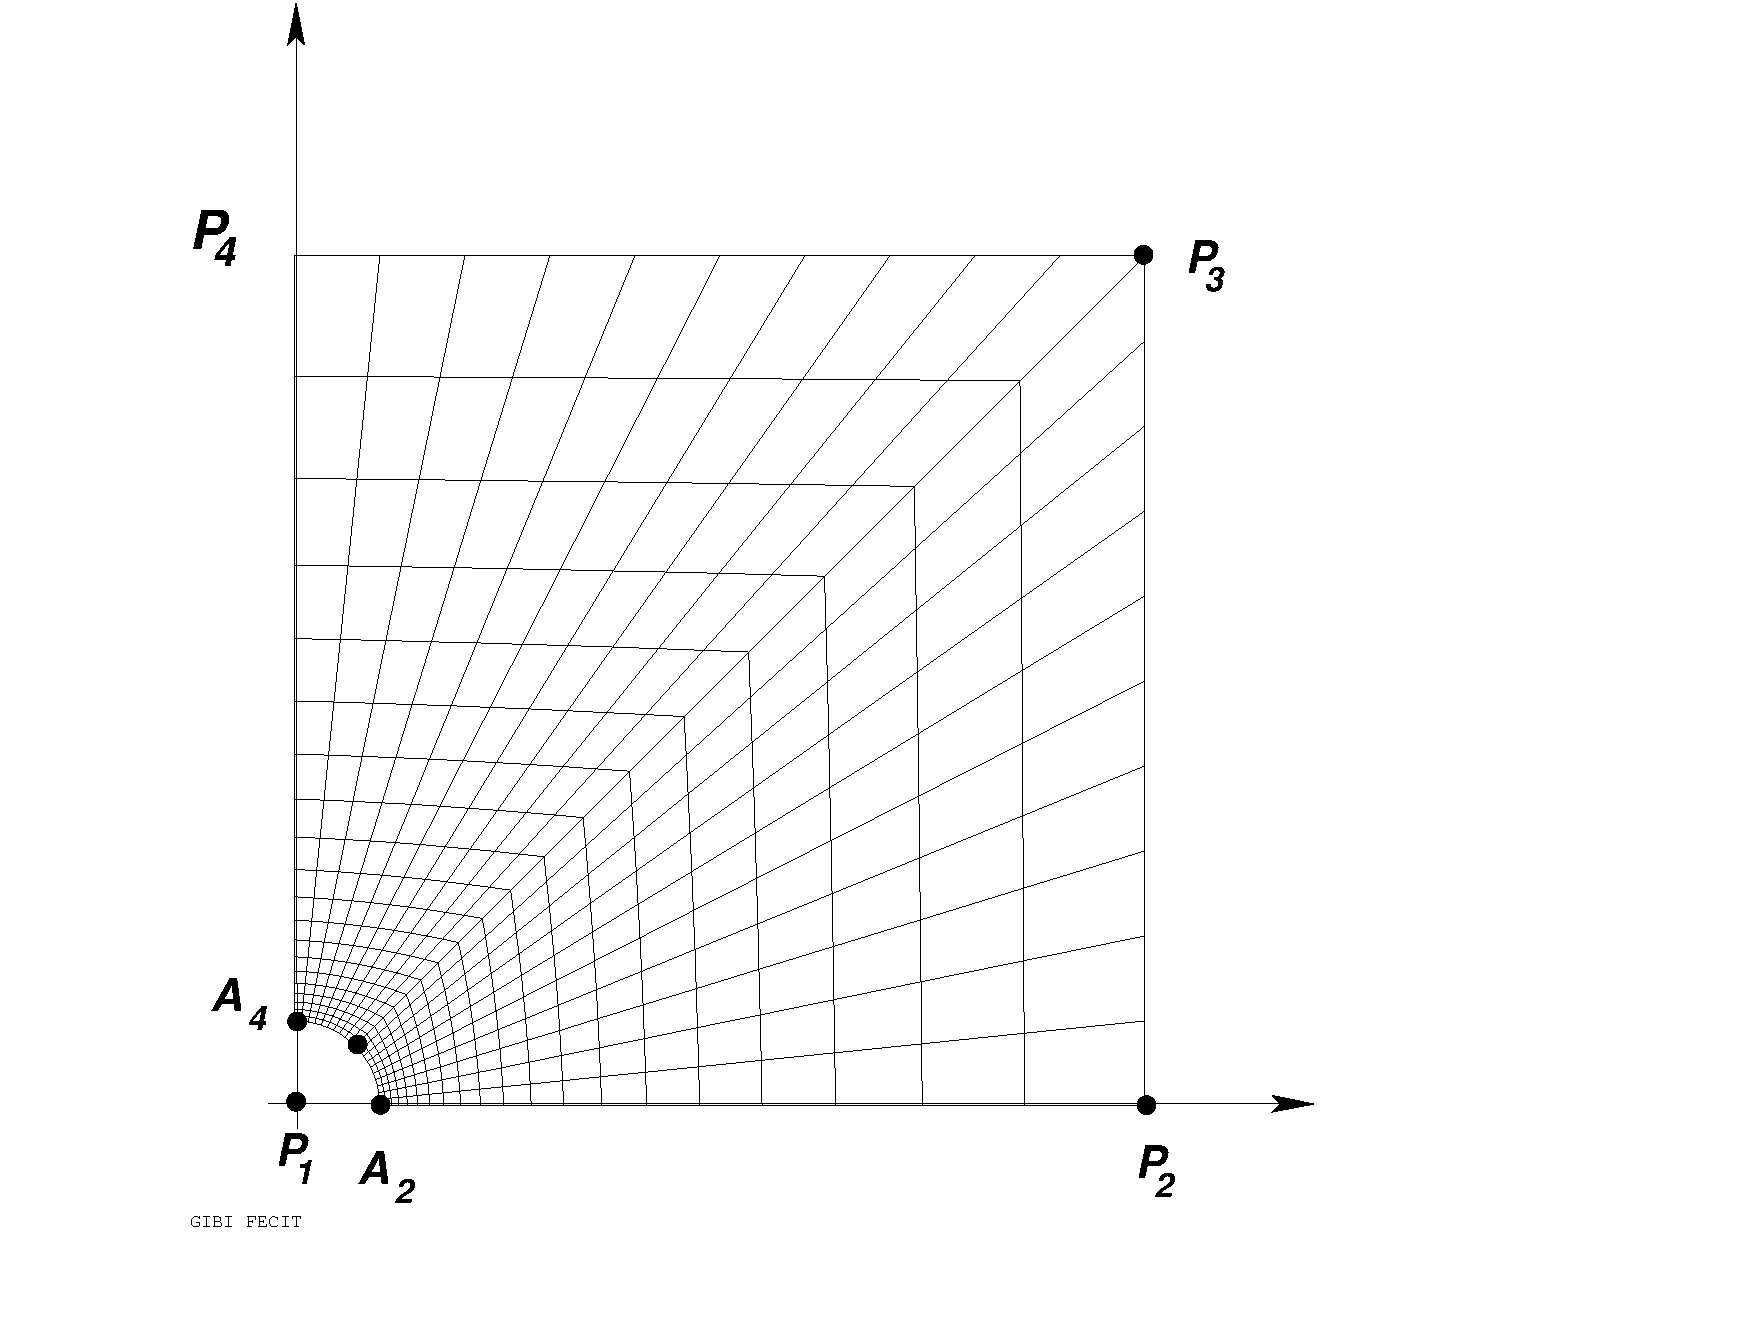
\includegraphics[height=5.cm]{./FIG/trou}
}
\caption{The quarter of a plate with a hole, in tension}
\label{fig:castem:trou}
\end{figure}

\begin{gbox}{Operators for 2D mesh creation}
\begin{tabular}{ll}
\texttt{cont[our]} & recovers the boundary of a domain \\
\texttt{syme[trie]} & creates the symmetric of a given mesh   \\
\texttt{tour[ner]} & creates  a new rotated mesh from of a given one   \\
\texttt{plus} & creates  a new  mesh by adding a displacement to a given mesh   \\
\texttt{elim[iner]} & eliminates nodes with close coordinates \\
\texttt{dedo[ublement]} & doubles existing nodes (the opposite of \texttt{elim[iner]}) \\
\texttt{poin[t]} & selects a set nodes of a given mesh  \\
\texttt{elem[ent]} & selects elements of a given mesh  \\
\texttt{face} & selects the n-th face of a mesh in 2D or 3D  \\
\end{tabular}
\end{gbox}

\begin{castemcom}
The complete geometry of the quadrangular plate with the 
hole in the center can simply be created by completing 
the geometry through symmetry (operator \texttt{syme[trie]}). 

A series of geometrical points are now represented through 
different nodes, which can be shrunk into one unique node 
using the \texttt{elim[iner]} operator. The real number 
at the end of the last command is the tolerance, defining 
the neighborhood for which nodes are reduced to one 
single node.
\dindex{elim[iner]}{merge close nodes}
\index{dedoubler @ \texttt{dedo[ubler]}}

It is worth noticing that an inverse command equally 
exists \texttt{dedo[ubler]} which creates additional nodes (doubles) 
for existing nodes. An example of application is the 
creation of cracks. 

\dindex{elim[iner]}{merge close nodes}

\end{castemcom}
\begin{castemlines}
\begin{verbatim}
 
quart2 = dom syme 'DROIT' p1 p4;
half = (dom et quart2) syme 'DROIT' p1 p2;

plate = elim (dom et quart2 et half) 0.001;

\end{verbatim}
\end{castemlines}

A difficulty with the new geometry \texttt{plate} is that its 
points, border lines and nodes, do not have a distinct name. 
Surely, one can address these objects by their node or element
number, but this will not provide an intrinsic solution as 
is might change with a new parametrization of the geometry 
or simply a new run of the program. The problem is solved 
by the \texttt{poin[t]} and \texttt{elem[ent]} operators as
illustrated in the next lines.
 
\begin{castemcom}
The \texttt{poin[t]} command will select the points of the 
contour of the plate, \texttt{cont plate}, lying within 
$0.001$ of the line (fr. \texttt{'DROITE'} ) 
defined by the points 
$(0., \, -l_{dom})$ and $(1., \, -l_{dom})$.

Next in a similar way, the \texttt{elem[ent]} command will 
select the elements of contour of the plate, 
\texttt{cont plate}, lying (fr. \texttt{'APPUYE'} ) 
strictly (fr. \texttt{'STRICTEMENT'} ) on the set points 
\texttt{poi\_line}.
\dindex{poin[t]}{select points or nodes}
\dindex{elem[ent]}{select elements}

The result is finally plotted using \texttt{trac[er]}. 
One can remark that the colour of the points has been 
changed into green (fr. \texttt{vert}) for a better  
display.

\end{castemcom}
\begin{castemlines}
\begin{verbatim}

poi_line = (cont plate) poin 'DROITE' 
        (0. (-1. * ldom))
        (1. (-1. * ldom)) 0.001;
	       
ele_line = (cont plate) elem
    'APPUYE' 'STRICTEMENT' poi_line;
 
trace ((cont plate)
       et (poi_line coul vert)
       et (ele_line coul rouge));
\end{verbatim}
\end{castemlines}

\section{Example of a 3D mesh creation}
\label{sec:mesh:3d}

Most of the commands presented in the preceding section will 
equally function in a three dimensional environment, creating 
the embedded points, lines or surfaces. We shall briefly illustrate 
one of the construction commands.   

\begin{castemcom}

The passage from two to three dimensions can be done 
in the middle of a program, if so the third coordinate 
of all existing objects will automatically be 
set to $0.$. This can readily be observed by plotting 
the third coordinate of the \texttt{plate}.  

The two dimensional surface: \texttt{plate},
can be extruded using the \texttt{volu[me]} 
command into a three dimensional cube.  

The \texttt{enve[loppe]} command recovers the 
boundary of the mesh exactly as \texttt{cont[our]} 
in the two dimensional case.

The extremal sections of the extruded volume 
can be recovered as the $1$ and $2$ face of the \texttt{cube},
while the cylindrical surface of the extrusion will form 
the $3$ face.  

\index{face@ \texttt{face} of a volume}
\index{envelope@ \texttt{enve[loppe]}, boundary surface of a volume}

\index{plus@ \texttt{plus}, new mesh by a adding a displacement}

\end{castemcom}
\begin{castemlines}
\begin{verbatim}

opti dime 3 elem cub8;

trace plate (plate coor 3);

cube = plate volu tran nel (0. 0. ldom);

trace cach cube;

trace cach (enve cube);

trace cach (cube face 1);
trace cach (cube face 2);
trace cach (cube face 3);

\end{verbatim}
\end{castemlines}


\section{Surfaces of revolution and ruled surfaces}
\label{sec:mesh:revolution}

\cindex{surface of revolution}\cindex{ruled surface}%
\cindex{cylindrical shell}\cindex{hyperbolic paraboloid}%
\cindex{cooling tower}%
Two families of surface deserve their own section, because they are the
geometries the eigenvalue computations of chapter~\ref{chap:eigen} are built
on and because each is produced by a single operator: a \emph{surface of
revolution}, made by rotating a line about an axis, and a \emph{ruled
surface}, made by sweeping a straight segment between two guide curves.

\subsection*{A cylindrical shell}

The thin cylinder is the standard specimen for both vibration and buckling: it
has analytical solutions, and it buckles in a pattern of circumferential
lobes that is easy to see.

\begin{castemcom}
\op{rota} \dindex{rota[tion]}{surface of revolution}
\dindex{tour[ner]}{rotate an existing object} sweeps a line about an
axis -- a point in 2D, two points defining the axis in 3D -- through a given
angle, and returns the surface it generates. Here the generating line is the
vertical segment \op{lgen} at radius $R$, swept through $360^{\circ}$ about
the $z$ axis. Note that it must not be called \op{gene}: an object whose
first four characters match an operator destroys that operator for the rest
of the session, and \op{gene} is one.

The angle is in degrees, and its sign sets the orientation of the generated
elements, which matters as soon as you apply a pressure or a contact
condition to the surface.

\medskip
A full revolution closes on itself, so the first and last nodes coincide
geometrically but are distinct objects: \op{elim} merges them. Forget it and
the cylinder is a rolled sheet with a seam, which shows up as a spurious
mode.
\end{castemcom}
\begin{castemlines}
\begin{verbatim}
opti dime 3 elem qua4;

rcyl = 0.5;  hcyl = 2.;
nh   = 20;   ncirc = 48;

* axis of revolution
pa = 0. 0. 0.;
pb = 0. 0. 1.;

* generating line, at radius rcyl
* (do not call it "gene": that would
*  shadow the GENE operator)
g1 = rcyl 0. 0.;
g2 = rcyl 0. hcyl;
lgen = droi nh g1 g2;

cyl = lgen rota ncirc 360. pa pb;
cyl = elim cyl 1.e-6;

* the two rims, for the boundary
* conditions
bas  = cyl poin 'PLAN' pa
       (1. 0. 0.) (0. 1. 0.) 1.e-4;
haut = cyl poin 'PLAN' g2
       (1. 0. hcyl) (0. 1. hcyl) 1.e-4;

trace cach cyl;
\end{verbatim}
\end{castemlines}

\dindex{cara[cteristiques]}{geometric characteristics}%
\cindex{shell thickness}%
\noindent A shell needs a thickness, which is not part of the mesh but of the
\emph{characteristics}: \op{cara mod 'EPAI' 0.002;}. That object is passed
alongside the material everywhere a stiffness is built -- see
chapter~\ref{chap:eigen}, where forgetting it is the commonest cause of a
buckling computation that returns nonsense.

\subsection*{A hyperbolic paraboloid}

The hyperbolic paraboloid is the shape of a natural-draught cooling tower. It
is doubly curved, yet it is a \emph{ruled} surface: it can be generated by a
straight line sliding between two circles of different radii, at different
heights, rotated relative to one another. That is why such towers can be built
from straight reinforcement.

\begin{castemcom}
\op{regl[er]} \dindex{regl[er]}{ruled surface} \sindex{gene[ratrice]}
builds the ruled surface joining two lines. The two lines must be \emph{of the same type}, have
\emph{the same number of elements}, and be described \emph{in the same
direction} -- the operator joins node $i$ of one to node $i$ of the other, so
if the surface comes out twisted into an hourglass, reverse one of them with
\op{inve}.

That twist is in fact the point here: the hyperbolic paraboloid is obtained
precisely by offsetting the two circles by a fraction of a turn. Rotating the
upper circle by $0^{\circ}$ gives a cone or a cylinder; the more you rotate
it, the more pronounced the waist.

\medskip
In 3D a full circle is built with the \texttt{'ROTA'} form of \op{cerc}:
rotate a starting point through $360^{\circ}$ about the axis given by two
points. The element count must be the same on both circles.
\end{castemcom}
\begin{castemlines}
\begin{verbatim}
opti dime 3 elem qua4;

rbas = 2.;  rhau = 1.6;  htot = 5.;
nc   = 48;  nv   = 20;
alph = 40.;

o1 = 0. 0. 0.;
o2 = 0. 0. htot;
za = 0. 0. 1.;

* lower circle: rotate a1 by 360
* about the axis o1-za
a1 = rbas 0. 0.;
c1 = cerc nc 'ROTA' 360. a1 o1 za;

* upper circle, offset by alph
b1 = rhau 0. htot;
b1 = b1 tour alph o2 za;
c2 = cerc nc 'ROTA' 360. b1 o2 za;

* a full circle closes on itself:
* merge the coincident end nodes,
* exactly as for the cylinder
c1 = elim c1 1.e-9;
c2 = elim c2 1.e-9;

* the ruled surface between them
tour1 = c1 regl nv c2;

trace cach tour1;
\end{verbatim}
\end{castemlines}

\noindent Setting \op{alph} to zero returns a truncated cone, which is a
useful check that the two circles are correctly matched before you introduce
the twist. The waist radius and its height follow from the geometry, and
comparing them with the computed mesh is the quickest way to confirm the
surface is the one you intended.

\begin{optable}{Surfaces of revolution and ruled surfaces}
rota[tion] & surface swept by rotating a line about a point (2D) or an axis
             (3D) \\
regl[er]   & ruled surface joining two lines of identical type and element
             count \\
tran[slation] & surface swept by translating a line along a vector \\
tour[ner]  & rotates an existing object (point, line, mesh) \\
volu[me]   & volume swept by a surface \\
gene[ratrice] & surface generated by translating one line parallel to another \\
cara       & geometric characteristics -- shell thickness, beam section \\
\end{optable}

%\subsection*{Rigid mouvements}

\section{Deformation of meshes}
\label{sec:mesh:deform}

A mesh can be deformed to create a new mesh just by adding 
a desired displacement field as illustrated 
in the next example.

\begin{castemcom}
We first extract the three coordinate fields of the plate,
and create the field: $u_z = x^2 + y^2$. The field 
will be labelled as the $z$ component of a displacement 
field after changing the name of its component 
from \texttt{'SCAL'} to \texttt{'UZ'}. 

The new mesh is simply created by adding the 
displacement to the initial mesh using the \texttt{plus}
command.

Finally results are plotted using \texttt{trace} 
after the colouring of the new mesh in red (fr. rouge) 
using \texttt{coul[eur]}

\end{castemcom}
\begin{castemlines}
\begin{verbatim}

xx yy zz = coor plate;

uuz = (xx * xx) + (yy * yy);
uuz = exco uuz 'SCAL' 'UZ';

pshell = plate plus uuz;

trace cach (plate et (pshell coul rouge));

\end{verbatim}
\end{castemlines}

\section{Meshes built elsewhere}

The import and export of meshes from and towards \texttt{Cast3M} 
is of importance for a series of practical applications. This topic 
is discussed in chapter~\ref{chap:importexport}.

\section{Numbers and measures for meshes}

\begin{castemcom}
The number of nodes and the number of elements of a mesh are simply 
recovered by applying the \texttt{nbno[euds]} \texttt{nbel[ements]}
operators.

\texttt{noeu[d]} permits to recover the geometrical point corresponding to 
the node of a mesh. Note however that node numbers change whenever the mesh
is regenerated, so \texttt{poin proc}, which looks a point up by its
coordinates, is the safer choice in a file you intend to re-run. 

\bigskip 

The area of the created meshes is computed 
by the \texttt{mesu[rer]} operator and the \texttt{surf[ace]} option. Other option,
\texttt{long[ueur]} (fr. length) and \texttt{volu[me]}
enable the computation of a length and a volume for 
one and respectively three dimensional objects.    

\index{mesurer@\texttt{mesu[rer]}, measures length, areas and volumes}
\index{nbno@\texttt{nbno[euds]}, computes the number of nodes}
\index{nbel@\texttt{nbel[ements]}, computes the number of elements}
 
\end{castemcom}
\begin{castemlines}
\begin{verbatim}

list (nbno pshell);
list (nbel pshell);

pp = pshell noeud 347;

* better: a geometric lookup, which
* survives a change of mesh
pp = pshell poin proc (0.5 0.5);
list (coor 1 pp);

list (mesu pshell 'SURF');


\end{verbatim}
\end{castemlines}

\begin{gbox}{Other operators for mesh manipulation}
\begin{tabular}{ll}
\texttt{nbel[ements]} & computes the number of elements of a mesh \\
\texttt{nbno[euds]} & computes the number of nodes of a mesh \\
\texttt{noeu[d]} &  defines a point using its nodal number \\[2.mm]
\texttt{mesu[rer]} & measures the length, surface or volume of a mesh \\
\end{tabular}
\end{gbox}

\framepart{Summary}

\begin{gbox*}
\begin{itemize}
  \item \textbf{A mesh is built upward}, from points to lines, then to
  surfaces and volumes, in two and in three dimensions. Each operator takes
  objects of the level below, which is why a careless point costs you the
  whole volume.
  \item \textbf{\op{opti dime} comes first.} The dimension of the working
  space and the element type are settings, not arguments, and they have to
  be set before anything is meshed.
  \item \textbf{Meshes put side by side are not joined.} Coincident points
  built twice stay two points until \op{elim} merges them, and a
  computation on an unmerged mesh runs happily and gives the wrong answer.
  \item \textbf{What is shown here is a small part of the whole.} The
  operators of this chapter cover a wide range of manipulations but by no
  means all of them; the rest is in the examples, the notices, and the
  reports on the \texttt{Cast3M} site.
\end{itemize}
\end{gbox*}

\framepart{Exercises}


\exercise{Hyperbolic paraboloid}

The hyperbolic paraboloid is a ruled surface (fr. surface r\'egl\'ee) generated by a line 
that pertains to two circles. This type of structures is used as a refrigeration 
tower for electricity generating plants. 

{\small \textit{Hint} use the \texttt{regl[er]} operator}






\chapter{Elliptic problems: elasticity and heat transfer}
\label{chap:elasticity}

\framepart{Outline}

This chapter sets up and solves the two model elliptic problems: linear
elastic equilibrium and thermal equilibrium. The two are treated together
because in \texttt{Cast3M} they are literally the same sequence of operators
with different keywords -- build a model, attach a material, assemble a
matrix, impose boundary conditions, solve, post-process. Once you have the
elastic chain in your fingers the thermal one costs five minutes.

We continue with the plate with a hole meshed in
chapter~\ref{chap:meshing}.

\section{Variational formulation of the elastic equilibrium}

\todoeq{variational formulation -- see the corresponding chapter of the
lecture notes}

\section{General settings}

The construction of a finite element solution starts with the definition of
the main modelling assumptions: dimension of the space, coordinate system,
plane strain or plane stress, Fourier representation, and so on.

\begin{castemcom}
The dimension of the working space and the fundamental assumptions of the
computation are chosen with the \op{opti} command. The two options shown here
correspond to plane strain, i.e. \op{defo[rmation] plan[e]}
\dindex{defo[rmation] plan[e]}{plane strain} in cartesian coordinates, and to
axial symmetry, i.e. \op{axis} \dindex{axis}{axial symmetry} in cylindrical
coordinates.
\end{castemcom}
\begin{castemlines}
\begin{verbatim}
opti mode defo plan;

opti mode axis;
\end{verbatim}
\end{castemlines}

\noindent The chosen spatial configuration automatically assigns the standard
names of the components of the different fields. \textbf{You do not get to
choose these names, and you will need them constantly} -- every \op{exco},
every \op{bloq}, every plot refers to a component by name.

\begin{itemize}
\item \textbf{plane strain} (\op{defo[rmation] plan[e]}). Displacement fields
  are defined in a cartesian coordinate system $(x,y,z)$ as
  \[ \vect{u}(x,y,z)=u_{x}(x,y)\,\vect{e}_{x}+u_{y}(x,y)\,\vect{e}_{y} \]
  and the component names are:

  \begin{center}
  \begin{tabular}{@{}l@{\hspace{10mm}}l@{}}
    \textbf{field} & \textbf{component name}\\[1mm]
    displacement & \texttt{UX, UY}\\
    forces       & \texttt{FX, FY}\\
    strain       & \texttt{EPXX, EPYY, EPXY, EPZZ}\\
    stress       & \texttt{SMXX, SMYY, SMXY, SMZZ}\\
  \end{tabular}
  \end{center}

  Note that \texttt{EPZZ} and \texttt{SMZZ} are present: in plane strain
  $\varepsilon_{zz}=0$ but $\sigma_{zz}=\nu(\sigma_{xx}+\sigma_{yy})\neq0$,
  and it is a standard mistake to forget it when computing an equivalent
  stress by hand.

\item \textbf{axial symmetry} (\op{axis}). Displacement fields are defined in
  a cylindrical coordinate system $(r,\theta,z)$ as
  \[ \vect{u}(r,\theta,z)=u_{r}(r,z)\,\vect{e}_{r}+u_{z}(r,z)\,\vect{e}_{z} \]
  and the component names become:

  \begin{center}
  \begin{tabular}{@{}l@{\hspace{10mm}}l@{}}
    \textbf{field} & \textbf{component name}\\[1mm]
    displacement & \texttt{UR, UZ}\\
    forces       & \texttt{FR, FZ}\\
    strain       & \texttt{EPRR, EPZZ, EPRZ, EPTT}\\
    stress       & \texttt{SMRR, SMZZ, SMRZ, SMTT}\\
  \end{tabular}
  \end{center}

  Here the hoop terms \texttt{EPTT}, \texttt{SMTT} carry the
  $\theta\theta$ component. In an axisymmetric computation the mesh must lie
  in the half-plane $r\geq0$, with $r$ as the first coordinate.
\end{itemize}

\noindent The complete list for every modelling option is in the notice of
\op{mode[le]} on the website~\cite{Cast3M:web}; the exact set also depends on
the element, so check it there rather than trusting this table for an element
type not used in this booklet.

\begin{optable}{General settings}
opti[on] dime n   & space dimension $n=1,2,3$ \\
opti[on] mode plan defo & cartesian coordinates, plane strain \\
opti[on] mode plan cont & cartesian coordinates, plane stress \\
opti[on] mode axis      & cylindrical coordinates, axisymmetric \\
opti[on] mode four[ier] n & cylindrical coordinates, Fourier expansion up to
                            $n$ harmonics \\
opti[on] mode trid[imensionnel] & cartesian coordinates, three-dimensional \\
\end{optable}

\section{Elasticity -- \texttt{Cast3M} problem setting}

\subsection{Boundary conditions and solution method}

The method of solution used by \texttt{Cast3M} is based on the Lagrangian
relaxation of the displacement boundary conditions, as explained for example
in~\cite{Bonnet:2007}. The variational principle
of the preceding section transforms into

\noindent which, after discretisation, leads to the linear
system~\cite{Bonnet:2007}

\begin{equation}
\begin{bmatrix} K & A^{T} \\ A & 0 \end{bmatrix}
\begin{bmatrix} U \\ \lambda \end{bmatrix}
=
\begin{bmatrix} F \\ U^{D} \end{bmatrix}
\label{eq:elas:lagrange}
\end{equation}

\noindent in which the stiffness matrix $[K]$ is defined with respect to
\emph{all} nodal displacements, with no distinction between values imposed by
the boundary conditions and the others. The imposed displacements enter
through the projection matrix $[A]$ and the imposed values $[U^{D}]$. The
traction boundary conditions and the body forces define the vector $[F]$.

The practical consequence of \eqref{eq:elas:lagrange} is the one that
surprises newcomers: \textbf{imposing a boundary condition adds unknowns to
the system} -- the Lagrange multipliers $\lambda$ -- rather than removing
them. Those multipliers are the reaction tractions, which is why they can be
recovered afterwards with \op{reac}.

\begin{castemcom}
The \op{mode[le]} \dindex{mode[le]}{model} operator associates to a given mesh
a finite element, i.e. a specific shape function in the variational principle
(here linear functions by default, the \texttt{QUA4} element), a mechanical
problem setting \op{mecanique}, and a linear isotropic elastic constitutive
law. Other problem settings are \op{thermique}, \op{liquide}, \op{darcy},
\ldots

The choice of the material behaviour determines the number and the names of
the parameters that must be supplied next through the \op{mate[riaux]}
\dindex{mate[riaux]}{material} operator, as well as the structure of the
internal variables of the model.

The stiffness matrix $[K]$ is then computed with \op{rigi[dite]}
\dindex{rigi[dite]}{stiffness} from the elastic information provided before.
\end{castemcom}
\begin{castemlines}
\begin{verbatim}
mod = dom mode mecanique
          elastique isotrope;

mat = mod mate 'YOUN' 2.e11 'NU' 0.3;

KK = rigi mod mat;
\end{verbatim}
\end{castemlines}

\begin{castemcom}
To construct the projection matrices $[A]$, which reduce the displacement
vector to the part of the boundary where $[U^{D}]$ is applied, we use
\op{bloq[uer]} \dindex{bloq[uer]}{block a degree of freedom}. The
corresponding right-hand side is then built from $[A]$ and $[U^{D}]$ with
\op{depi} \dindex{depi}{imposed displacement} (fr. \emph{déplacement imposé}).

Note that \op{bloq[uer]} and \op{depi} do not merely build $[A]$ and
$[U^{D}]$: they also create the new degrees of freedom corresponding to the
Lagrange multipliers. Mechanically these multipliers are the tractions $[T]$
on that part of the boundary, unknown before the system is solved. You can
see them by listing the object: \op{list Ad34;}.

Here \op{d12} and \op{d41} carry the symmetry conditions of the quarter
plate ($u_y=0$ on the lower edge, $u_x=0$ on the left edge), while the block
on \op{d34} is the loading: the upper edge is given the imposed displacement
$u_y=0.1$.
\end{castemcom}
\begin{castemlines}
\begin{verbatim}
Ad12 = bloq uy d12;
Ad41 = bloq ux d41;
Ad34 = bloq uy d34;

ud34 = depi Ad34 0.1;

AA = Ad12 et Ad41 et Ad34;
\end{verbatim}
\end{castemlines}

\begin{castemcom}
The system is finally solved by calling \op{reso[udre]}
\dindex{reso[udre]}{solve}. Only the non-zero components of the right-hand
side have to be specified -- here only \op{ud34}; the rest is completed with
zeros automatically.
\end{castemcom}
\begin{castemlines}
\begin{verbatim}
u = reso (KK et AA) ud34;
\end{verbatim}
\end{castemlines}

\begin{castemcom}
Listing the components of the displacement field shows the expected
\texttt{UX} and \texttt{UY}, and also a new component \texttt{LX}: the
Lagrange multiplier, which carries $[T]$.

To obtain the underlying traction vector we use \op{reac[tion]}
\dindex{reac[tion]}{reaction forces}, which turns the multipliers back into
nodal forces on the blocked boundary. Summing them is the standard way to get
the resultant force on a boundary -- for instance to plot a force/displacement
curve.
\end{castemcom}
\begin{castemlines}
\begin{verbatim}
list (extr u 'COMP');

td34 = reac u Ad34;

* resultant on d34
ftot = resu (exco td34 'FY');
\end{verbatim}
\end{castemlines}

\subsection{Have the boundary conditions removed every rigid body motion?}
\label{sec:elas:ense}

\cindex{rigid body motion}\cindex{under-restrained structure}%
\cindex{singular stiffness matrix}%
Before solving anything, it is worth asking whether the blocked degrees of
freedom actually hold the structure. A body that can still translate or
rotate as a whole has a singular stiffness matrix, and the symptoms are
unmistakable once you know them: the solver fails, or it returns
displacements of absurd magnitude with a sensible-looking stress field
superposed on them.

In two dimensions a body has three rigid body motions -- two translations and
one rotation -- and in three dimensions six. Every one of them must be
removed by the boundary conditions. Counting them by hand on the quarter
plate is easy; on a real assembly of several parts, with symmetry conditions
and contact, it is not, and this is where most "the solver does not converge"
problems actually live.

\texttt{Cast3M} will answer the question directly.

\begin{castemcom}
\op{ense[mble]} \dindex{ense[mble]}{rigid body modes of a stiffness matrix}
takes an assembled stiffness -- \emph{including its blocking matrices} -- and
returns a \op{solution} object containing the \emph{mouvements d'ensemble},
the rigid body modes that the matrix still permits.

\medskip
\textbf{The test is the number of modes it finds.} None means the structure
is properly restrained and you can solve. One or more means it is not, and
each mode it returns \emph{is} a motion your \op{bloq} conditions failed to
suppress -- so you do not have to guess which one is missing: plot it.

\op{tire} \dindex{tire[r]}{extract a mode from a solution object} pulls out
mode number \texttt{n} as a displacement field, which is then drawn with
\op{defo} like any mode shape.
\end{castemcom}
\begin{castemlines}
\begin{verbatim}
* KK is the stiffness, AA the
* assembled blocking matrices
mmm = ense (KK et AA);

* how many rigid modes remain?
nrig = dime mmm;
mess 'rigid body modes left: ' nrig;

* ... and what are they?
si (nrig > 0);
  repeter brig nrig;
    i  = &brig;
    di = tire mmm 'DEPL' 'RANG' i;
    trac (defo dom di 1. rouge);
  fin brig;
finsi;
\end{verbatim}
\end{castemlines}

\noindent The complement of \op{bloq} is therefore \op{ense}: one imposes the
conditions, the other checks that they were enough. Running it once on every
new model costs nothing and saves a great deal of time.

\medskip
Two situations where you will want it even though nothing has gone wrong:

\begin{itemize}
\item \textbf{a free-free structure, deliberately.} A modal analysis of an
  unrestrained body -- an aircraft, a satellite panel, a specimen hanging on
  soft springs -- is supposed to have rigid body modes, and
  \op{vibr[ation]} will return them as modes at (numerically) zero frequency.
  Knowing from \op{ense} how many to expect is exactly how you tell a genuine
  zero-frequency mode from a mesh that has fallen apart;
\item \textbf{before a buckling computation.} \op{flambage} works on a
  stiffness that must be non-singular, so an under-restrained model gives
  meaningless critical loads rather than an error. Chapter~\ref{chap:eigen}
  returns to both of these.
\end{itemize}

\noindent A related use of the word: \op{rela 'ENSE'}, in
section~\ref{sec:elas:rela}, imposes that a component be \emph{equal} over a
whole boundary -- a rigid platen. The two are unconnected beyond the shared
French word \emph{ensemble}, "as a whole".

\medskip
\noindent\textbf{A note on the name.} The operator is \op{ense[mble]}, not
\op{enve}. \op{enve[loppe]} is the meshing operator of
section~\ref{sec:mesh:3d} that extracts the boundary surface of a volume
(and, in a second form, the envelope of a set of oscillator spectra). The two
are easy to confuse from memory and do entirely different things.

\begin{optable}{Plots}
trac[er] & plots different objects \\
trac[er] model field & plots a field defined on elements \\
trac[er] geometry field & plots a field defined at nodes \\
trac[er] geometry & plots a mesh \\
dess[iner] evolution & plots the graph of a function \\
evol[ution] & graph of a function defined by lists of numbers \\
evol[ution] 'CHPO' \ldots & extracts the evolution of a field along a path \\
\end{optable}

\noindent The results can be post-processed in a number of ways, as shown in
the next examples.

\begin{castemcom}
To plot the norm of the displacement vector
\[ \norm{u}=\sqrt{u_{x}^{2}+u_{y}^{2}} \]
we extract the components with \op{exco} \dindex{exco}{extract a component}
(fr. \emph{extraire composante}), combine them algebraically, and plot with
\op{trac[er]}.

The second argument of \op{exco} is the component to take, the third the name
to give it in the result: renaming to \texttt{'SCAL'} is what lets the two
components be multiplied together afterwards -- fields are only combined
component by component, by name.

As displacement fields are defined by their nodal values, the underlying mesh
must be given for the plot.
\end{castemcom}
\begin{castemlines}
\begin{verbatim}
uux = exco u 'UX' 'SCAL';
uuy = exco u 'UY' 'SCAL';

trace uux dom;

unorm = (((uux*uux) + (uuy*uuy))**0.5);
trace unorm dom;
\end{verbatim}
\end{castemlines}

\begin{castemcom}
Strains and stresses are computed with \op{epsi[lon]}
\dindex{epsi[lon]}{strain} and \op{sigm[a]} \dindex{sigm[a]}{stress}; the
operations correspond to the matrix computations
\begin{align}
\varepsilon &= [B][U] \\
\sigma      &= [C][B][U]
\end{align}
with $[C]$ the elasticity matrix. Note that \op{sigm} needs the material in
addition to the model, whereas \op{epsi} does not -- strain is a purely
kinematic quantity.

Both results are \op{mchaml} objects, defined at the Gauss points. The names
of their components can be listed with \op{extr[aire]}.
\end{castemcom}
\begin{castemlines}
\begin{verbatim}
eps = epsi mod u;
sig = sigm mod mat u;

list (extr eps 'COMP');
list (extr sig 'COMP');
\end{verbatim}
\end{castemlines}

\begin{castemcom}
Another operator corresponds to $[B^{T}]$ and computes the nodal forces
associated with a given stress field:
\begin{equation}
[F]=[B^{T}]\sigma
\end{equation}
which is the discrete counterpart of $\ddiv\sigma$ in a continuum
formulation. \op{bsig[ma]} \dindex{bsig[ma]}{nodal forces from a stress field}

A good sanity check on any converged solution: these nodal forces must vanish
everywhere except at the boundary, where they equal the reactions. If they do
not, the solution is not in equilibrium.
\end{castemcom}
\begin{castemlines}
\begin{verbatim}
f = bsigm mod sig;

trace dom (exco f 'FX');
trace dom (exco f 'FY');
\end{verbatim}
\end{castemlines}

\begin{optable}{Strains and stresses}
epsi[lon] & computes the strain tensor \\
sigm[a]   & computes the stress tensor \\
bsig[ma]  & computes the nodal forces corresponding to a stress tensor \\
tres[ca]  & computes the Tresca norm of the stress tensor \\
vmis[es]  & computes the von Mises norm,
            $\sqrt{\tfrac{3}{2}\,\dev\sigma\bcddot\dev\sigma}$ \\
prin[cipales] & computes the principal values of the stress tensor \\
@plotpri  & plots the principal values (user-defined procedure) \\
\end{optable}

\begin{castemcom}
To plot the components of a strain or stress tensor we apply \op{trac[er]}
directly and adjoin the \emph{model}, not the mesh, so that the position of
the Gauss points where the values are defined is known.

This is the practical difference between a \op{chpoint} and a \op{mchaml}:
\op{trace \textit{mesh} \textit{field}} for the first,
\op{trace \textit{model} \textit{field}} for the second.
\end{castemcom}
\begin{castemlines}
\begin{verbatim}
trace mod sig;
\end{verbatim}
\end{castemlines}

\begin{castemcom}
Different scalar measures derived from the stress tensor are computed
directly: the Tresca and von Mises norms with \op{tres[ca]} and
\op{vmis[es]} \dindex{vmis[es]}{Mises stress norm}, the principal values and
their directions with \op{prin[cipales]}.

\op{@plotpri} is a user-defined procedure which plots the principal stresses
interactively. Procedures whose names start with \op{@} are user
contributions rather than standard operators -- see
chapter~\ref{chap:importexport} on how to load them.
\end{castemcom}
\begin{castemlines}
\begin{verbatim}
sigvm = vmis mod sig;
sigtr = tres mod sig;
sigpr = prin mod sig;

@plotpri sig mod;
\end{verbatim}
\end{castemlines}

\begin{castemcom}
It is often more informative to display the evolution of a stress component
along a path than over the whole domain. Here we plot $\sigma_{yy}$ along the
border of the circular hole, where the stress concentration is.

We first list the components of the stress field. We then interpolate the
$\sigma_{yy}$ component -- \texttt{'SMYY'} -- from the Gauss points to the
nodes using \op{chan[ger]} with the \texttt{'CHPO'} option
\dindex{chan[ger] 'CHPO'}{change a field into nodal values}: a path extraction
needs nodal values. Finally \op{evol[ution]} with the \texttt{'CHPO'} option
extracts the values along the path \op{(arc23 et arc34)} and \op{dess[iner]}
draws the graph.
\sindex{evol[ution], 'CHPO', along a path}
\end{castemcom}
\begin{castemlines}
\begin{verbatim}
list (extr sig 'COMP');

sigyy = chan 'CHPO' mod
             (exco sig 'SMYY');

ev1 = evol 'CHPO' sigyy
           (arc23 et arc34);
dess ev1;
\end{verbatim}
\end{castemlines}

\noindent For the plate with a hole in tension this is the computation that
should return the classical stress concentration factor $K_t=3$ for an
infinite plate; comparing your value with 3 is the natural first validation of
the whole chain, and the discrepancy tells you how much the finite width of
the plate matters.

\subsection{Other applied forces: pressure, weight, \ldots}

The load in the previous example was an imposed displacement only, so the
exterior load vector was $[F]=[0]$ and the program completed it with zeros.
The next examples show how surface tractions and body forces are imposed.

\begin{optable}{Applied forces}
forc[e]    & distributes a given force over a set of nodes \\
pres[sion] & computes the nodal force distribution for a given pressure \\
coor[donnees] & computes the coordinate fields of a given mesh \\
mass[e]    & computes the mass matrix \\
manu 'CHPO' & constructs a nodal field by hand \\
\end{optable}

\begin{optable}{Creation of stiffness-type matrices}
rigi[dite]     & stiffness matrix \\
mass[e]        & mass matrix \\
cond[uctivite] & conductivity matrix \\
capa[cite]     & capacity matrix \\
conv[ection]   & stiffness corresponding to a convection boundary condition \\
\end{optable}

\subsection{Surface traction and applied pressure}

The main operators for constructing applied forces are \op{forc[e]}
\sindex{forc[e]} and \op{pres[sion]} \sindex{pres[sion]}.

\begin{castemcom}
The \op{coor} \dindex{coor[donnees]}{coordinate fields} operator builds the
coordinate fields of a mesh. Here we recover $x$ and $y$ at each point of the
line \op{d23}.

\op{pres} computes the nodal force field corresponding to the pressure
distribution $p(x,y)=3x^{2}$. A model is needed because the computation
integrates the pressure against the shape functions of the underlying
elements (see~\cite{Bonnet:2007}) -- a pressure is not simply divided equally
between nodes. Note
that this model must be built \emph{on the loaded boundary} \op{d23}, not on
the surface \op{dom}: it is the line elements that are integrated over. This
is a frequent source of errors.

Finally the normal pressure distribution \op{fnor} is turned into a tangential
traction \op{ftan} by exchanging the components of the vector field and
changing one sign, i.e. by rotating it by $90^{\circ}$.
\end{castemcom}
\begin{castemlines}
\begin{verbatim}
* the model must live on the loaded
* line, not on the surface
mod23 = d23 mode mecanique
            elastique isotrope;

xx yy = coor d23;

fnor = pres mass mod23 (3.* (xx * xx));

ftan = (exco fnor 'FY' 'FX') et
       (-1. * (exco fnor 'FX' 'FY'));
\end{verbatim}
\end{castemlines}

\noindent To impose a Hertzian pressure distribution, for example a parabola
centred on the left end of the loaded edge,
\[
p(x)=\begin{cases}
p_{max}\,(a_{p}^{2}-x^{2}) & \text{if } \abs{x}<a_{p}\\
0 & \text{if } \abs{x}\ge a_{p}
\end{cases}
\]
we proceed in the same way, with one extra ingredient.

\begin{castemcom}
\op{manu[el]} \dindex{manu[el]}{create a field by hand} constructs a constant
nodal field, which is what lets a constant appear in an otherwise
field-valued formula: $a_p$ has to become a field before $a_p^2-x^2$ can be
formed.

\op{masq[uer]} \dindex{masq[uer]}{mask, characteristic function} builds the
characteristic function of the condition
$x<a_{p}$ -- a field equal to 1 where the condition holds and 0 elsewhere.
Multiplying by it is how one writes a piecewise definition in
\textsc{gibiane}; there is no \op{si} test inside a field expression. Here
the edge runs from $x=0$, so $x<a_p$ and $\abs{x}<a_p$ select the same
points; on an edge straddling the origin you would need the product of two
masks, as in the inclusion example below.

The final nodal force distribution is assembled by multiplying the two.
\end{castemcom}
\begin{castemlines}
\begin{verbatim}
xx = coor 1 d34;

ap   = ldom / 3.;
pmax = 1.e8;

one = manu 'CHPO' d34 1 'SCAL' 1.;

px  = pmax * (((ap * one) ** 2)
              - (xx ** 2));

mask = (xx masq 'INFERIEUR' ap);
px   = px * mask;

mod34 = d34 mode mecanique
            elastique isotrope;
fp = pres mass mod34 px;
\end{verbatim}
\end{castemlines}

\subsection{Body forces}

\begin{castemcom}
To build a body force taking the density of the body into account, the
density \texttt{RHO} is added to the material and the mass matrix is computed
with \op{mass[e]}.

If the gravitational acceleration is defined as the nodal field \op{g}, the
body force is simply the product of the mass matrix with it: $[F]=[M]\{g\}$.
That is the discrete form of $\int_\Omega \rho\, \vect{g}\cdot\vect{v}$, and
it is the correct way to apply gravity -- distributing the total weight
equally over the nodes is not.
\end{castemcom}
\begin{castemlines}
\begin{verbatim}
mat = mod mate 'YOUN' 2.e11 'NU' 0.3
               'RHO' 2000.;

MM = mass mod mat;

g = manu 'CHPO' dom 1 'UY' -9.81;

fvol = MM * g;
\end{verbatim}
\end{castemlines}

\subsection{Thermal expansion}

\cindex{thermal expansion}\cindex{thermoelasticity}%
\cindex{dilatation coefficient}%
The thermal expansion of a heated body is a loading like any other, and it is
worth treating here because it is the commonest way a thermal computation
feeds back into a mechanical one. It follows directly from the thermoelastic
constitutive law
\begin{equation}
  \tens{\sigma} = \tens{C} : \left( \tens{\varepsilon} - \tens{a}\,\theta \right)
\label{eq:elas:thermoelastic}
\end{equation}
where $\tens{C}$ and $\tens{a}$ are the fourth-order tensor of elastic moduli
and the second-order tensor of thermal dilatation, and $\theta$ is the field of
temperature difference between the initial and the actual configuration. In the
elastic problem setting $\theta$ is known: it plays the role of a loading.

For an isotropic material this simplifies to
\begin{equation}
  \tens{\sigma} = \lambda \tr (\tens{\varepsilon} - \alpha \theta \tens{I}) \tens{I}
   + 2 \mu (\tens{\varepsilon} - \alpha \theta \tens{I})
\end{equation}
and, in the absence of body forces, the balance equation
$\ddiv \tens{\sigma} = 0$ becomes
\begin{equation}
   \ddiv \left[ \tens{C} : \tens{\varepsilon} \right]
   = \ddiv \left[ \tens{C} : \left( \tens{a}\,\theta \right) \right]
\end{equation}

\noindent The right-hand side is the point: a temperature field acts exactly
like a distributed body force, generated by the incompatibility of the thermal
expansion. That is why a uniform temperature rise on an unconstrained body
produces no stress at all, while the same rise on a constrained or
inhomogeneous body does.

These steps map one to one onto the \textsc{gibiane} program.

\begin{castemcom}
The thermal expansion coefficient must be declared in the material data. For
an isotropic elastic material the component name is \texttt{'ALPH'}.

\medskip
In this example the temperature field $\theta$ is \op{delta\_th}. The operator
\op{thet[a]} \dindex{thet[a]}{thermal stress field} computes, from the
material data and the temperature field, the thermal stress field
\[ \op{sig\_th} = \tens{C} : \left( \alpha\,\theta\,\tens{I} \right) \]
The equivalent body forces follow from \op{bsig[ma]}, whose role was described
earlier in this chapter.

The solution is then obtained with the standard \op{reso[udre]}, from the
stiffness matrix \op{KK}, the matrices of the imposed displacement conditions
\op{AA}, and the body force field \op{f\_th}.

\medskip
Note that \op{thet} measures the temperature from a reference value
\texttt{'TALP'}, which defaults to zero: \op{delta\_th} is a temperature
\emph{difference}, not an absolute temperature.
\end{castemcom}
\begin{castemlines}
\begin{verbatim}
mod = dom mode mecanique
          elastique isotrope;
mat = mod mate 'YOUN' 2.e11 'NU' 0.3
               'ALPH' 1.e-5;

* ... boundary conditions as before,
*     giving KK and AA ...

delta_th = manu 'CHPO' dom 1 'T' 1000.;

sig_th = thet mod mat delta_th;
f_th   = bsigm mod sig_th;

u = reso (KK et AA) f_th;
\end{verbatim}
\end{castemlines}

\noindent The stress actually carried by the body is \emph{not} \op{sig\_th}:
it is the stress computed from the resulting displacement minus the thermal
part, i.e. \op{(sigm mod mat u) - sig\_th}. Forgetting that second term is the
classic error in a thermoelastic computation, and it shows up as a non-zero
stress in a body that is free to expand.

\subsection{Other constraints on displacements}
\label{sec:elas:rela}

Blocking a degree of freedom to a given value is not the only kind of boundary
condition. \cindex{rigid platen}\cindex{linear constraint between unknowns}%
A frequent requirement is that a part of the boundary stay flat or
move as a rigid whole -- a loading platen, a symmetry condition on a surface
that is free to translate -- i.e. that all the displacement components of the
points of a line $\ell$ be equal to each other:
\begin{equation}
   \vect{u}(\vect{x}) = \text{constant}
   \qquad \forall \vect{x} \in \ell \subset \partial \Omega
\end{equation}
The constant itself is left free, and is fixed afterwards -- for instance by
imposing the displacement at one particular point of the line, as in the
example below.

\dindex{rela[tion]}{constraint on the displacement field}

\begin{castemcom}
The operator \op{rela[tion]} with the option \texttt{'ENSE'}
(fr. \emph{ensemble}) builds a stiffness matrix -- again a set of Lagrange
multipliers -- imposing that the \texttt{UY} component of the displacement
field be the same at every node of the line \op{d34}.

To fix the value of that unknown constant we impose the displacement at the
single point \op{p3}. The rest is as before: assemble all the matrices and
solve with \op{reso[udre]}.

\medskip
This is what you want for a rigid platen pressing on the plate: the surface
stays flat, but the traction distribution under it is computed rather than
assumed -- which is exactly the difference between this and \op{bloq}-ing the
whole line to a fixed value.
\end{castemcom}
\begin{castemlines}
\begin{verbatim}
Ad34 = rela 'ENSE' 'UY' d34;

Ap3 = bloq 'UY' p3;
up3 = depi Ap3 0.3;

AA = Ad12 et Ad41 et Ad34 et Ap3;

u = reso (KK et AA) up3;
\end{verbatim}
\end{castemlines}

\noindent \op{rela[tion]} imposes many other kinds of constraint, equalities
and inequalities alike: rigid body motion (\texttt{'CORI'}), sliding relations
between two meshes (\texttt{'GLIS'}), tying mid-side nodes to corner nodes
(\texttt{'MILI'}), coupling a pipe surface to its centre line
(\texttt{'TUYA'}), and so on. See its notice for the full list.

\begin{optable}{Conditions on displacements}
bloq[uer] & blocks a degree of freedom to an imposed value \\
rela[tion] & stiffness matrix for a linear relation between degrees of
             freedom \\
rela[tion] 'ENSE' & imposes one component to be equal over a whole mesh \\
rela[tion] 'CORI' & imposes a rigid body motion \\
depi      & right-hand side associated with an imposed value \\
reac[tion] & recovers the reaction associated with a constraint \\
\end{optable}

\subsection{Spatially varying material coefficients}

We have seen that spatially varying boundary tractions are easily defined with
\op{coor[donnees]} and \op{masq[uer]}. The same construction gives varying
material parameters. The example below places a square inclusion in a plate --
a two-material composite.

\begin{castemcom}
The example runs on its own square mesh \op{plaq} rather than on the plate
with the hole, since an inclusion spanning $0.2\le x,y\le 0.8$ would otherwise
overlap the hole.

The characteristic field of the inclusion, \op{D\_CAR}, is built as the
product of four masks and takes the value 1 inside the square and 0 outside;
\op{M\_CAR} is its complement.

The distributions of Young's modulus and Poisson's ratio are then
interpolations between the two materials weighted by these two fields.

The next step is the one to pay attention to. Material parameters live at the
Gauss points of the elements, not at the nodes, so the nodal fields must be
converted with \op{chan[ger]}
\dindex{chan[ger] 'CHAM'}{change from nodal to element field} using the
keywords \texttt{'CHAM'} (fr. \emph{champ}) and \texttt{'RIGIDITE'}, which
define the intended use and the header of the new field.
\dindex{chpo}{change from nodal to element field}%
\dindex{mchml}{change from nodal to element field} The component name
also has to be changed from \texttt{'SCAL'} to \texttt{'YOUN'} and
\texttt{'NU'} with \op{nomc} \dindex{nomc}{rename a component}, because
\op{mate} identifies its arguments by component name.

Material and stiffness matrix are then created as usual, the only difference
being that the arguments are fields rather than numbers.
\end{castemcom}
\begin{castemlines}
\begin{verbatim}
* a plain square of side 1, not the
* plate with the hole: the inclusion
* below would overlap the hole
opti dime 2 elem qua4;
c1 = 0. 0.;  c2 = 1. 0.;
c3 = 1. 1.;  c4 = 0. 1.;
plaq = dall (droi 20 c1 c2) (droi 20 c2 c3)
            (droi 20 c3 c4) (droi 20 c4 c1);

mod = plaq mode mecanique
           elastique isotrope;

X_min = 0.2; X_max = 0.8;
Y_min = 0.2; Y_max = 0.8;

xx yy = coor plaq;

D_CAR = xx masq 'SUPERIEUR' X_min;
D_CAR = D_CAR *
        (xx masq 'INFERIEUR' X_max);
D_CAR = D_CAR *
        (yy masq 'SUPERIEUR' Y_min);
D_CAR = D_CAR *
        (yy masq 'INFERIEUR' Y_max);

one   = manu 'CHPO' plaq 1 'SCAL' 1.;
M_CAR = one - D_CAR;

* aluminium and copper
YG_al = 69.e9;  NU_al = 0.33;
YG_co = 117.e9; NU_co = 0.35;

YG_r = (YG_co * M_CAR)
       + (YG_al * D_CAR);
NU_r = (NU_co * M_CAR)
       + (NU_al * D_CAR);

yg_c = chan 'CHAM'
       (nomc 'YOUN' YG_r) mod 'RIGIDITE';
nu_c = chan 'CHAM'
       (nomc 'NU'  NU_r) mod 'RIGIDITE';

trace mod yg_c;

mat = mate mod 'YOUN' yg_c 'NU' nu_c;
rig = rigi mod mat;
\end{verbatim}
\end{castemlines}

\noindent Two remarks on this example. First, the moduli in the original
version of these notes were identical for the two materials
($33\,$GPa and $\nu=0.32$ for both aluminium and copper), so the computation
returned a homogeneous plate; the values above are the usual ones and actually
produce an inclusion. Second, a continuously varying distribution is obtained
in exactly the same way, replacing the masks by any expression in \op{xx} and
\op{yy}.

\begin{optable}{Manipulation of fields}
chan[ger] & changes the field type by interpolation \\
manu[el]  & creates new objects \\
nomc      & changes the name of a component \\
exco      & extracts a component, optionally renaming it \\
masq[uer] & characteristic function of a condition \\
\end{optable}

\section{Thermal equilibrium -- \texttt{Cast3M} problem setting}
\label{sec:elas:thermal}

The steady thermal equilibrium problem is
\begin{equation}
  \ddiv \left( k \, \grad \theta \right) + r = 0
  \qquad \text{in } \Omega
\label{eq:thermal:equilibrium}
\end{equation}
with $k$ the conductivity and $r$ a volume heat source, completed by imposed
temperature, imposed flux or convection conditions on the boundary. It has
exactly the structure of the elastic problem, and is solved by exactly the
same sequence of operators.

\begin{castemcom}
The finite element model and the material properties are declared exactly as
in the elastic case, with \op{mode[le]} and \op{mate[riaux]}; only the
keywords change.

The resolution of~\eqref{eq:thermal:equilibrium} depends only on the
conductivity \texttt{K}. If the
density \texttt{RHO} and the specific heat \texttt{C} are also given, the
capacity matrix can be computed as well, which is what the transient
computation of chapter~\ref{chap:heat} will need.

\op{cond[uctivite]} and \op{capa[cite]} play exactly the roles that
\op{rigi[dite]} and \op{mass[e]} play in elasticity -- same objects, same
algebra, same solver.
\sindex{thermique} \sindex{conductivite} \sindex{capacite}
\end{castemcom}
\begin{castemlines}
\begin{verbatim}
mod = dom mode thermique isotrope;

mat = mod mate 'K' 1. 'RHO' 1. 'C' 1.;

KK = cond mod mat;
CC = capa mod mat;
\end{verbatim}
\end{castemlines}

\begin{castemcom}
An imposed temperature on the boundary uses the same Lagrange multiplier
technique as in elasticity: \op{bloq[uer]} builds the projection matrix and
\op{depi} the associated right-hand side.

The name of the degree of freedom is \texttt{'T'}, which is also the name of
the component of the temperature field.
\end{castemcom}
\begin{castemlines}
\begin{verbatim}
Ad23 = bloq 'T' d23;
AA   = Ad23;

Fd23 = depi Ad23 4.;
\end{verbatim}
\end{castemlines}

\begin{castemcom}
The nodal ``forces'' equivalent to a boundary heat flux are obtained with
\op{flux} \dindex{flux}{boundary heat flux}. As with \op{pres}, the model is
needed because the flux is integrated against the shape functions.
\end{castemcom}
\begin{castemlines}
\begin{verbatim}
Fd34 = flux mod 2. d34;
\end{verbatim}
\end{castemlines}

\begin{castemcom}
The convection boundary condition
\[ -k\derp{\theta}{n}=h\,(\theta-\theta_{\infty}) \]
is mathematically of a different type: it involves the unknown $\theta$ on the
boundary itself. It therefore contributes \emph{both} an extra conductivity
matrix \op{KK\_hol}, defined by the exchange coefficient $h$, \emph{and} a
nodal flux \op{Fhole} defined by $h$ and the environment temperature
$\theta_{\infty}$. Both must be added to the system.
\sindex{convection, boundary condition}

Radiation conditions of the type
$-k\derp{\theta}{n}=\varepsilon_{r}\sigma_{\!SB}(\theta^{4}-\theta_{\infty}^{4})$,
with $\sigma_{\!SB}$ the Stefan--Boltzmann constant and $\varepsilon_{r}$ the
emissivity, are
nonlinear and cannot be handled in this linear setting; a first approximation
is a temperature-dependent exchange coefficient $h=h(\theta)$, and the proper
treatment goes through \op{pasapas}.
\end{castemcom}
\begin{castemlines}
\begin{verbatim}
mod_hol = (arc23 et arc34)
          mode convection;
mat_hol = mod_hol mate 'H' 1.;

KK_hol = cond mod_hol mat_hol;
Fhole  = conv mod_hol mat_hol
              'T' 200.;
\end{verbatim}
\end{castemlines}

\begin{castemcom}
A distributed heat source inside the body is created with \op{sour[ce]}
\dindex{sour[ce]}{volume heat source}, given its value, the domain it applies
to and the model.
\end{castemcom}
\begin{castemlines}
\begin{verbatim}
Fsource = sour mod 100. dom;
\end{verbatim}
\end{castemlines}

\begin{castemcom}
The temperature field is finally obtained by solving the assembled system with
\op{reso[udre]}. Note that \emph{both} the conductivity matrix \op{KK} of
the domain and the convection matrix \op{KK\_hol} of the boundary condition
appear in the stiffness term -- that is what distinguishes a convection
condition from an imposed flux, which contributes only to the right-hand side.

All the right-hand side contributions are concatenated with \op{et}.
\end{castemcom}
\begin{castemlines}
\begin{verbatim}
KTOT = KK et KK_hol et AA;
FTOT = Fd23 et Fd34 et Fhole
            et Fsource;

TT = reso KTOT FTOT;

trace TT dom;
\end{verbatim}
\end{castemlines}

\noindent Varying boundary temperatures, fluxes or convection coefficients,
and volume heat sources, are imposed with the same \op{coor}/\op{masq}
constructions as the varying pressure above.

\begin{optable}{Thermal problem setting}
mode[le] \ldots thermique & thermal finite element model \\
mode[le] \ldots convection & model carrying a convection boundary condition \\
cond[uctivite] & conductivity matrix \\
capa[cite] & capacity matrix \\
flux & nodal flux equivalent to a boundary heat flux \\
conv[ection] & nodal flux of a convection condition \\
sour[ce] & nodal flux of a volume heat source \\
\end{optable}

\section{An unexpected use of the thermal solver}
\label{sec:elas:torsion}

\cindex{Laplace equation}\cindex{thermal analogy}%
\cindex{Saint-Venant torsion}\cindex{warping function}%
\cindex{torsional rigidity}\cindex{torsion centre}%
\cindex{Timoshenko beam}\cindex{shear correction coefficient}%
\cindex{beam cross-section properties}%
Before leaving the thermal operators, one idiom worth knowing, because it is
the kind of thing that distinguishes someone who knows a finite element code
from someone who only knows one physics in it: \textbf{the thermal solver can
be used to solve any Laplace problem}, whatever it means physically.

The classical example is the \emph{Saint-Venant torsion} of a prismatic beam.
When a bar of arbitrary cross-section is twisted, plane sections do not stay
plane -- they warp out of plane by a function $\varphi(x,y)$ which satisfies,
over the cross-section $S$,
\begin{equation}
  \Delta \varphi = 0 \quad \text{in } S,
  \qquad
  \derp{\varphi}{n} = y\,n_{x} - x\,n_{y} \quad \text{on } \partial S
\label{eq:elas:warping}
\end{equation}
and from which the torsional rigidity $J$ follows by integration over the
section. That is a Laplace equation with a prescribed normal derivative --
mathematically identical to steady heat conduction with an imposed boundary
flux, which is exactly what the previous section solved.

So the cross-section is meshed as a 2D domain, given a \emph{thermal} model
with unit conductivity, and the warping function is computed as if it were a
temperature.

\begin{castemcom}
The model is \op{thermique} even though the problem is mechanical. The
conductivity is set to 1, so that \op{cond} assembles exactly the discrete
Laplacian.

\op{flux} imposes the boundary term of~\eqref{eq:elas:warping}. A pure
Neumann problem is defined only up to a constant, so one point must be fixed
-- any point will do, and the choice shifts $\varphi$ without changing $J$.

The torsional rigidity is then an integral over the section, obtained with
\op{intg} \dindex{intg[rer]}{integrate a field over a domain}.
\end{castemcom}
\begin{castemlines}
\begin{verbatim}
opti dime 2 elem tri3;

* sect = mesh of the cross-section
modt = sect mode thermique isotrope;
matt = modt mate 'K' 1.;

KK = cond modt matt;

* fix the constant at one point
p0  = sect poin proc (0. 0.);
bl0 = bloq 'T' p0;
f0  = depi bl0 0.;

* ... boundary flux, built from the
* normal to the contour (see text)

phi = reso (KK et bl0) (fbord et f0);

trace phi sect;
\end{verbatim}
\end{castemlines}

\sindex{"@Torsion (procedure)}\cindex{Maxwell--Betti theorem}%
\noindent This is the basis of the \texttt{@Torsion} procedure presented at
the Club Cast3M by Gornet~\cite{Gornet:club2017}, which computes from a
meshed cross-section its area and centroid, its principal second moments, the
warping function, the torsional rigidity, the position of the torsion centre
-- located through the Maxwell--Betti reciprocal theorem -- and the shear
correction coefficients, i.e. everything a Timoshenko beam model needs. It is
validated there on triangular, rectangular, L- and C-sections, on hollow
sections with fillets, and on NACA aerofoil profiles.

That procedure is not distributed with \texttt{Cast3M} and the presentation
gives only extracts of it, so it would have to be rebuilt from the slides.
The construction above is the core of it, and rebuilding the rest is a good
project: see the exercises.

%%%
\section{Material coefficients varying with temperature}

Suppose now that a law correlates a material property $P$ with the temperature
$\theta$ -- the Young modulus $E(\theta)$, say, or the dilation coefficient
$\alpha(\theta)$. The question is how to compute the spatial distribution of
$P$ in the presence of an inhomogeneous temperature field $\theta(x)$, i.e.
\[ P(x)=P(\theta(x)) \]

\noindent The construction is the one used above for the inclusion, with the
masks replaced by an interpolation of the measured law. In practice there are
two routes: either evaluate the law directly as an algebraic expression in the
temperature field, or tabulate it as an \op{evolution} and interpolate with
\op{ipol}. The second is what you want when the law comes from measurements,
and is what the data-reading section of chapter~\ref{chap:importexport} is
for.

\framepart{Summary}

The whole chapter is one sequence of five operators, and it is the same
sequence for elasticity and for heat conduction:

\begin{center}
\begin{tabular}{@{}l@{\hspace{8mm}}l@{\hspace{8mm}}l@{}}
                     & \textbf{elasticity} & \textbf{thermal} \\[1mm]
model                & \op{mode \ldots mecanique} & \op{mode \ldots thermique} \\
material             & \op{mate 'YOUN' 'NU'}      & \op{mate 'K' 'RHO' 'C'} \\
matrix               & \op{rigi}                  & \op{cond}, \op{capa} \\
boundary conditions  & \op{bloq} + \op{depi}      & \op{bloq 'T'} + \op{depi} \\
solution             & \op{reso}                  & \op{reso} \\
\end{tabular}
\end{center}

\begin{gbox*}
\begin{itemize}
  \item \textbf{Imposed conditions add unknowns rather than removing them.}
  They are handled by Lagrange multipliers, and those multipliers are the
  reactions, recovered with \op{reac}.
  \item \textbf{Every load that is not a nodal force is built the same way.}
  Pressure, weight, thermal expansion: form a field, integrate it against
  the shape functions with the operator that belongs to it (\op{pres},
  \op{mass}, \op{thet}), and add the result to the right-hand side.
  \item \textbf{Spatially varying data is built from the coordinates.}
  Whether it is a load or a material parameter: \op{coor} and \op{masq} to
  build it, \op{chan} to move it to the Gauss points.
\end{itemize}
\end{gbox*}

\framepart{Exercises}

\exercise{Stresses and strains in a plate with a hole} Run the program
  presented in this chapter and:
  \begin{itemize}
  \item check the stress distribution for all types of applied force: body
    force, applied surface pressure, tangential traction;
  \item compute the solution for a given resultant force applied to the upper
    face of the plate, using both \op{forc[e]} and \op{pres[sion]}. Explain
    the difference between the two;
  \item compare the computed stress concentration factor with the
    theoretical value $K_t=3$, and study how it changes as the ratio
    $r/L$ of hole radius to plate width decreases.
  \end{itemize}
  See the file \texttt{traction\_trou.dgibi}.

\exercise{Mesh convergence} Repeat the computation with \op{nel} equal to
  5, 10, 20 and 40 and plot the maximum von Mises stress against the number of
  degrees of freedom. At which refinement is the result converged to within
  1\%? Compare the convergence of the displacement with that of the stress and
  explain why they differ.

\exercise{Elastic and thermal example files} Run the elasticity example
  files \texttt{elas*.dgibi} and the thermal ones \texttt{ther*.dgibi} from
  the \texttt{cast3m\_dir/dgibi} directory of your installation, and read the
  notes in \texttt{cast3m\_dir/dgibi/annotated\_testing\_files\_98.pdf} and
  on the \textbf{Exemples} page of the website.

\exercise{Torsion by the thermal analogy} Following
  section~\ref{sec:elas:torsion}, compute the warping function and the
  torsional rigidity $J$ of a \emph{circular} section, for which the exact
  answer is $J=\pi R^{4}/2$ and the warping is identically zero -- a good
  check that your boundary term is right. Then do a square section, where
  $J \simeq 0.1406\,a^{4}$ and the warping is not zero, and plot it. Finally
  a thin rectangle, and compare with $J\simeq\frac{1}{3}ab^{3}$.

  \emph{Going further:} rebuild the rest of \texttt{@Torsion} -- centroid,
  principal axes and second moments, torsion centre, shear coefficients --
  as a procedure of your own taking a meshed section and returning a table.
  It is a satisfying small project and the result is genuinely useful.

\exercise{Thermoelastic coupling} Compute the temperature field of the
  plate with the hole with the boundary conditions of
  section~\ref{sec:elas:thermal}, then use it as a loading for the elastic
  problem through a thermal dilation coefficient \texttt{'ALPH'}. Where are
  the largest stresses, and why are they not where the temperature is
  highest?

\chapter{Parabolic and hyperbolic problems: transient analysis}
\label{chap:heat}

\framepart{Outline}

This chapter adds time. We take the heat conduction equations in the
transient regime and study the heating of the plate with a hole, then do the
same for elastodynamics with the Newmark algorithm.

Both problems could be handed to the \op{pasapas} operator, which is what you
would do in production and what chapter~\ref{chap:plasticity} describes. We
program the time loop explicitly here instead, because writing the algorithm
out in \textsc{gibiane} is the quickest way to understand what \op{pasapas}
does for you -- and because the same loop structure is what you will reuse
for any algorithm of your own.

\section{Transient heat transfer}

\noindent This section continues the thermal problem of
section~\ref{sec:elas:thermal}: the model \op{mod}, the material \op{mat}
and the blocked boundary \op{Ad23} are the ones built there, so run that
section first (or restore its objects with \op{rest}).


Recall that the family of algorithms presented in the lecture notes rests on
the equation

\begin{equation}
\left[\frac{1}{\Delta t}M + \theta K\right] T_{n+1}
=
\left[\frac{1}{\Delta t}M - (1-\theta) K\right] T_{n}
+ \theta F_{n+1} + (1-\theta) F_{n}
\label{eq:heat:theta}
\end{equation}

\cindex{transient analysis}\cindex{time integration}%
\cindex[theta-method]{$\theta$-method}\cindex{Crank--Nicolson scheme}%
\cindex{implicit scheme}\cindex{explicit scheme}\cindex{stability, unconditional}%
\noindent which determines $T_{n+1}$ knowing $T_{n}$. Here $M$ is the
capacity matrix, $K$ the conductivity matrix, and $\theta\in[0,1]$ is a
parameter: $\theta=0$ gives the explicit Euler scheme, $\theta=1$ the implicit
one, $\theta=1/2$ the Crank--Nicolson scheme, which is second-order accurate.
Only $\theta\geq1/2$ is unconditionally stable.

\begin{castemcom}
We start by fixing the time step and the algorithm parameter. The choice
$\theta=1$ gives an implicit and therefore unconditionally stable algorithm --
the safe default while you are debugging.

Note that with $\theta=1$ there is no restriction on $\Delta t$ for stability,
but there very much is one for accuracy: the solution will be smooth and
wrong rather than oscillatory and wrong.
\end{castemcom}
\begin{castemlines}
\begin{verbatim}
dt    = 0.1;
theta = 1.;
\end{verbatim}
\end{castemlines}

\begin{castemcom}
\sindex{table, as a history container}\cindex{time step}%
The conductivity and capacity matrices are built first. Both are objects of
\op{rigidite} type, which is why they can be combined with \op{et} and
multiplied by scalars exactly like stiffness matrices.

The two matrices of the algorithm follow directly from
\eqref{eq:heat:theta}. They are assembled once, outside the loop -- this is
the whole point of a constant time step, since \op{Matnpun} is the only
matrix that has to be factorised.
\end{castemcom}
\begin{castemlines}
\begin{verbatim}
KK = cond mod mat;
MM = capa mod mat;

Matnpun = ((1./dt) * MM)
          et (theta * KK);
Matn    = ((1./dt) * MM)
          et ((theta - 1.) * KK);
\end{verbatim}
\end{castemlines}

\begin{castemcom}
The matrix $A$ corresponding to the temperature imposed on the exterior
boundary is built as in the steady case, and the maximum exterior temperature
\op{Td} is fixed.
\end{castemcom}
\begin{castemlines}
\begin{verbatim}
Td = 1.;

Ad23 = bloq 'T' d23;
AA   = Ad23;
\end{verbatim}
\end{castemlines}

\begin{castemcom}
The tables of temperature fields and of imposed temperatures are initialised.
A \op{table} indexed by the step number is the natural \textsc{gibiane}
container for a history: \op{T . n} is the field at step $n$, and the whole
history stays available for post-processing after the loop.
\end{castemcom}
\begin{castemlines}
\begin{verbatim}
T = table;
T . 0 = manu 'CHPO' dom 1 'T' 0.;

F = table;
F . 0 = depi Ad23 0.;
\end{verbatim}
\end{castemlines}

\begin{castemcom}
The computation is then the resolution of \eqref{eq:heat:theta} at each time
step.

Two points of \textsc{gibiane} syntax are worth noting. \op{\&boucle} is the
iterator of the loop named \op{boucle}, and it runs from 1, which is why
\sindex{\&, loop iterator}%
\op{n} is defined as \op{\&boucle - 1} so that the indices match the tables
starting at 0. And the index of a table may be any expression, provided it is
bracketed: \op{F . (n + 1)}.

Here the imposed boundary temperature ramps linearly from 0 to \op{Td} over
the \op{ndt} steps.

Note the two different combinations in the right-hand side: \op{+} adds two
nodal fields defined on the same degrees of freedom, whereas \op{et}
\emph{concatenates} contributions living on different ones -- here the
volume term and the Lagrange-multiplier term of the blocked boundary. They
are not interchangeable.
\end{castemcom}
\begin{castemlines}
\begin{verbatim}
ndt = 20;

repeter boucle ndt;
  n = &boucle - 1;

  F . (n + 1) = depi Ad23
                ((n + 1) * Td / ndt);

  Fn = (theta * (F . (n + 1))) +
       ((1. - theta) * (F . n));

  T . (n + 1) = reso (Matnpun et AA)
                ((Matn * (T . n)) et Fn);
fin boucle;
\end{verbatim}
\end{castemlines}

\begin{castemcom}
After the loop the history is in the table, and any point value can be
followed in time by extracting it step by step into a \op{listreel} and
building an \op{evolution}.

\op{extr} with a point as last argument takes the value of a nodal field at
that point. This is the idiom you will use over and over for time histories.
\end{castemcom}
\begin{castemlines}
\begin{verbatim}
tt   = prog;
thi  = prog;
pA   = dom poin proc (0.5 0.5);

repeter post (ndt + 1);
  n = &post - 1;
  tt  = tt  et (prog (n * dt));
  thi = thi et
     (prog (extr (T . n) 'T' pA));
fin post;

dess (evol manu 'time' tt
               'T' thi);
\end{verbatim}
\end{castemlines}

\section{Example in dynamic analysis}

\cindex{dynamics, elastic}\cindex{Newmark algorithm}%
\cindex{average acceleration scheme}\sindex{dyne}%
\cindex{modal projection}\cindex{wave propagation}%
As an example of dynamic analysis we take the equations of linear elasticity
in the dynamic regime and program the Newmark algorithm in \textsc{gibiane}.

As for the transient thermal problem, this type of problem can be solved with
the \op{pasapas} operator. A variant based on the projection of the
displacement field on a modal basis is available through the \op{dyne}
operator, which is far cheaper when many time steps are needed and the
response is dominated by a few modes.

The Newmark family rests on the prediction/correction pair

\begin{align}
\tilde{U}_{n+1} &= U_{n} + \Delta t\,\dot{U}_{n}
   + \tfrac{1}{2}\Delta t^{2}(1-2\beta)\,\ddot{U}_{n} \\
\dot{\tilde{U}}_{n+1} &= \dot{U}_{n} + \Delta t (1-\gamma)\,\ddot{U}_{n}
\end{align}

\noindent followed by the resolution of
$\left[M+\beta\Delta t^{2}K\right]\ddot{U}_{n+1}
 = F_{n+1}-K\tilde{U}_{n+1}$
and the update
$U_{n+1}=\tilde{U}_{n+1}+\beta\Delta t^{2}\ddot{U}_{n+1}$,
$\dot{U}_{n+1}=\dot{\tilde{U}}_{n+1}+\gamma\Delta t\,\ddot{U}_{n+1}$.

\begin{castemcom}
A bar of length \op{ldom} and height \op{hdom} is built starting from the line
defining its left boundary, \op{dgauche}, and generating the mesh with
\op{tran[slation]}. The right boundary is recovered as face 3 of the
generated surface.
\end{castemcom}
\begin{castemlines}
\begin{verbatim}
* beware: this redefines ldom, which
* chapter 3 also uses
ldom = 50.; hdom = 1.;
p1 = 0. 0.; p2 = 0. hdom;

nlelem = 100; nhelem = 2;

dgauche = droi nhelem p1 p2;
dom     = dgauche tran nlelem
                  (ldom 0.);
ddroite = dom face 3;
\end{verbatim}
\end{castemlines}

\begin{castemcom}
The model and the material follow. Note that \texttt{'RHO'} is compulsory
here: without a density there is no mass matrix and no dynamics.

With $E=1$, $\rho=1$ the wave speed is $c=\sqrt{E/\rho}=1$, so a wave crosses
the 50-unit bar in 50 time units -- convenient for checking the results
against the analytical solution.
\end{castemcom}
\begin{castemlines}
\begin{verbatim}
mod = dom mode mecanique
          elastique isotrope;
mat = mod mate 'RHO' 1.
               'YOUN' 1. 'NU' 0.3;
\end{verbatim}
\end{castemlines}

\begin{castemcom}
The parameters of the computation: the time step \op{dt} and the algorithm
parameters $\beta$ and $\gamma$.

The values $\beta=1/4$, $\gamma=1/2$ give the average acceleration scheme,
which is implicit, second-order accurate, unconditionally stable and
conserves energy. They are the standard choice and the one to use unless you
have a reason not to.
\end{castemcom}
\begin{castemlines}
\begin{verbatim}
ndt   = 200;
dt    = 1.;
beta  = 0.25;
gamma = 0.5;
\end{verbatim}
\end{castemlines}

\begin{castemcom}
The boundary conditions: the left end of the bar is clamped, and a rectangular
pulse of force is applied at the right end during the first few instants.

Building the load as a table indexed by step number, as here, keeps the time
dependence explicit and readable. Note that the table must be filled for \emph{every} step the time loop will
read: a missing entry raises an error rather than returning zero. That is why
the loop opposite fills all \op{ndt}$+1$ entries, setting the two steps of
the pulse to \op{fimp} and all the others to zero.

\dindex{char[gement]}{loading history}%
For a long history it is more convenient to define an \op{evolution} and use
\op{char[gement]}, as in chapter~\ref{chap:plasticity}.
\end{castemcom}
\begin{castemlines}
\begin{verbatim}
AA = bloq 'DEPL' dgauche;

f0   = forc ddroite (0. 0.);
fimp = forc ddroite (-1. 0.);

F = table;
repeter bload (ndt + 1);
  k = &bload - 1;
  si ((k ega 1) ou (k ega 2));
    F . k = fimp;
  sino;
    F . k = f0;
  finsi;
fin bload;
\end{verbatim}
\end{castemlines}

\begin{castemcom}
The stiffness matrix $[K]$ and the mass matrix $[M]$ are assembled, and from
them the matrix $[S]=[M]+\beta\Delta t^{2}[K]$ -- the only one that will be
inverted during the algorithm, and the reason the implicit Newmark scheme
costs one factorisation rather than one per step.
\end{castemcom}
\begin{castemlines}
\begin{verbatim}
KK = rigi mod mat;
MM = mass mod mat;

SS = MM et
     ((beta * (dt ** 2.)) * KK);
\end{verbatim}
\end{castemlines}

\begin{castemcom}
Displacements $[U]$, velocities $[\dot{U}]$ and accelerations $[\ddot{U}]$ are
initialised. The initial acceleration is not chosen freely: it is obtained
from the equation of motion at $t=0$, i.e. by solving
$M\ddot{U}_0 = F_0 - K U_0$, which here reduces to $M\ddot{U}_0 = F_0$ since
$U_0=0$.
\end{castemcom}
\begin{castemlines}
\begin{verbatim}
U   = table;
dU  = table;
ddU = table;

U  . 0 = manu 'CHPO' dom 2
              'UX' 0. 'UY' 0.;
dU . 0 = manu 'CHPO' dom 2
              'UX' 0. 'UY' 0.;

ddU . 0 = reso (MM et AA) (F . 0);
\end{verbatim}
\end{castemlines}

\begin{castemcom}
And finally the time increment loop, in three stages: prediction, computation
of the acceleration, correction and update.

The three stages are written out so that the structure of the Newmark scheme
stays visible; in production \op{pasapas} does the same thing.
\end{castemcom}
\begin{castemlines}
\begin{verbatim}
repeter boucle ndt;
  n = &boucle - 1;

* ** prediction
  Upred  = (U . n)
    + (dt * (dU . n))
    + ((0.5 * dt * dt
        * (1. - (2.*beta))) * (ddU . n));
  dUpred = (dU . n)
    + ((dt * (1. - gamma)) * (ddU . n));

* ** acceleration
  ddU . (n + 1) = reso (SS et AA)
    ((F . (n+1)) - (KK * Upred));

* ** correction and update
  U  . (n + 1) = Upred
    + ((dt * dt * beta) * (ddU . (n+1)));
  dU . (n + 1) = dUpred
    + ((dt * gamma) * (ddU . (n+1)));
fin boucle;
\end{verbatim}
\end{castemlines}

\framepart{Summary}

\begin{gbox*}
\begin{itemize}
  \item \textbf{Adding time changes the loop, not the operators.} Both
  algorithms in this chapter have the same shape: assemble the constant
  matrices once outside the loop, keep the history in a \op{table} indexed
  by step number, and solve one linear system per step.
  \item \textbf{A constant time step is worth having.} The only matrix that
  is factorised is the one multiplying the unknown at $n+1$; keep the step
  constant and it is factorised once.
  \item \textbf{Two parameters decide whether the result means anything}:
  the scheme parameters -- $\theta$ for the heat equation,
  $(\beta,\gamma)$ for Newmark -- and the time step. $\theta\ge1/2$ and
  $\gamma=1/2$, $\beta=1/4$ are unconditionally stable and are the defaults
  to use until you have a reason not to.
  \item \textbf{Stability is not accuracy.} An over-large step gives a
  smooth, plausible and wrong answer.
\end{itemize}
\end{gbox*}

\framepart{Exercises}

\exercise{Stability of the $\theta$-scheme} Rerun the transient thermal
  computation with $\theta=0$ (explicit Euler) and increase $\Delta t$ until
  the solution oscillates. Compare the critical step with the theoretical
  stability limit. Then repeat with $\theta=1/2$ and $\theta=1$ and verify
  that no such limit exists.

\exercise{Energy conservation in Newmark} For the bar with no applied
  load after the initial pulse, compute at each step the kinetic energy
  $\tfrac12 \dot{U}^{T}M\dot{U}$ and the elastic energy
  $\tfrac12 U^{T}KU$, and plot their sum. Verify that it is conserved for
  $\gamma=1/2$ and dissipated for $\gamma>1/2$.

\exercise{Wave propagation} Plot the displacement of the free end of the
  bar against time and identify the round-trip travel time of the wave.
  Compare with $2L/c$.

\chapter{\textbf{Eigenvalue problems: vibrations and buckling}}
\label{chap:eigen}

\section*{Outline}
\addcontentsline{toc}{section}{\texorpdfstring{\hskip14mm}{} Outline}

The two previous chapters solved $KU=F$: given a load, find the response.
This chapter asks a different question -- for which loads, or at which
frequencies, does the structure respond \emph{without} being driven? Both
answers come from an eigenvalue problem, and in \texttt{Cast3M} both are
reached by the same route.

\begin{align}
  \text{free vibration:} \qquad & \left[K - (2\pi f)^{2} M\right] X = 0
  \label{eq:eigen:vibr} \\[1mm]
  \text{buckling:} \qquad & \left[K + \lambda\, K_{\sigma}\right] X = 0
  \label{eq:eigen:flam}
\end{align}

\cindex{eigenvalue problem}\cindex{vibration, free}\cindex{buckling}%
\cindex{natural frequency}\cindex{critical load}%
\noindent In the first, $M$ is the mass matrix and the eigenvalue is a
frequency. In the second, $K_{\sigma}$ is the \emph{geometric} stiffness
produced by a reference stress state, and the eigenvalue $\lambda$ is the
factor by which that reference load must be multiplied to make the structure
buckle. The mathematics is the same; only the second matrix changes.

We use the cylinder and the hyperbolic paraboloid of
section~\ref{sec:mesh:revolution}.

\section{Free vibration}

\subsection{Setting up the problem}

A vibration computation needs exactly one thing beyond a static one: a mass
matrix, which means a density in the material.

\begin{castemcom}
The model, the material and the stiffness are built exactly as in
chapter~\ref{chap:elasticity}; \op{mass[e]} \dindex{mass[e]}{mass matrix}
builds the mass matrix from the same model and material.

\sindex{coq4}\cindex{shell element}\cindex{shell thickness}%
\textbf{\texttt{'RHO'} is compulsory.} Without a density there is no mass
matrix, and the eigenvalue problem is meaningless. A shell also needs its
thickness, supplied through \op{cara} \dindex{cara[cteristiques]}{geometric characteristics} and concatenated to the material with \op{et} -- the single
most common reason a modal computation returns absurd frequencies.

The boundary conditions enter the stiffness exactly as before. Here the lower
rim of the cylinder is clamped. Note that \op{bloq 'DEPL' 'ROTA'} blocks both
translations and rotations, which is what an encastred shell edge needs.
\end{castemcom}
\begin{castemlines}
\begin{verbatim}
opti dime 3 elem qua4;

mod = cyl mode mecanique
          elastique isotrope coq4;

mat = mod mate 'YOUN' 2.1e11
               'NU'   0.3
               'RHO'  7800.;
car = mod cara 'EPAI' 0.002;
mat = mat et car;

KK = rigi mod mat;
MM = mass mod mat;

bl = bloq 'DEPL' 'ROTA' bas;

KT = KK et bl;
\end{verbatim}
\end{castemlines}

\subsection{Computing the modes}

\op{vibr[ation]} \dindex{vibr[ation]}{eigenvalue problem, vibration} solves
\eqref{eq:eigen:vibr}. It offers four algorithms, and which one you pick
matters more than it looks:

\sindex{vibr[ation], 'PROC'[HE]}\sindex{vibr[ation], 'SIMU'[LTANE]}%
\sindex{vibr[ation], 'INTE'[RVALLE]}\sindex{vibr[ation], 'IRAM'}%
\cindex{Lanczos algorithm}\cindex{Arnoldi algorithm}%
\begin{optable}{The four options of \texttt{vibr[ation]}}
'PROC'[HE] & the \texttt{n} modes nearest each frequency of a given list.
             Robust, and the one to use when you already know roughly where
             the modes are \\
'SIMU'[LTANE] & the \texttt{n} modes nearest one frequency, by Lanczos.
                Efficient when many modes are wanted -- \textbf{the sensible
                default} \\
'INTE'[RVALLE] & all modes in a frequency band, by bisection. The option to
                 use when the band matters rather than the count, but
                 generally far more expensive \\
'IRAM' & implicitly restarted Arnoldi, via \textsc{arpack}. The only option
         that accepts a damping matrix \\
\end{optable}

\begin{castemcom}
Here we ask for the ten lowest modes near zero, with \op{'SIMU'}. The
operator takes the stiffness and the mass matrix, in that order, and returns
a \op{table}.

\medskip
\textbf{The result structure is worth memorising}, because every
post-processing step goes through it. The table has an index \op{'MODES'},
itself a table indexed by mode number, and each entry holds:

\begin{itemize}[leftmargin=1.2em,itemsep=0pt,topsep=2pt]
\sindex{vibr[ation], 'MODES'}\sindex{'FREQUENCE'}%
\sindex{'DEFORMEE\_MODALE'}\sindex{'MASSE\_GENERALISEE'}%
\cindex{mode shape}\cindex{generalised mass}%
\item \texttt{'FREQUENCE'} -- the frequency, in Hz;
\item \texttt{'DEFORMEE\_MODALE'} -- the mode shape, a \op{chpoint};
\item \texttt{'MASSE\_GENERALISEE'} -- the generalised mass;
\item \texttt{'NUMERO\_MODE'} -- the mode number.
\end{itemize}

\noindent Frequencies come out in Hz, in whatever unit system the matrices
were built in -- so with SI data you get Hz, and with a density in
\texttt{g/mm}$^{3}$ you do not.
\end{castemcom}
\begin{castemlines}
\begin{verbatim}
nmod = 10;

res = vibr 'SIMU' 0. nmod KT MM;

* list the frequencies
lfreq = prog;
repeter bmod nmod;
  i  = &bmod;
  fi = res . 'MODES' . i . 'FREQUENCE';
  lfreq = lfreq et (prog fi);
  mess 'mode ' i ' : ' fi ' Hz';
fin bmod;
\end{verbatim}
\end{castemlines}

\begin{castemcom}
A mode shape is a \op{chpoint} like any displacement field, so it is plotted
with \op{defo} \dindex{defo[rmee]}{deformed shape} and \op{trac[er]}. Drawing
the undeformed shape with an amplification of \op{0.} and superposing it is
the usual way to make the mode legible.

\medskip
Remember that a mode shape has no physical amplitude -- it is normalised, here
by the generalised mass. Only its \emph{shape} and its frequency mean
anything; the numerical values of the displacements do not.
\end{castemcom}
\begin{castemlines}
\begin{verbatim}
repeter bdes nmod;
  i   = &bdes;
  di  = res . 'MODES' . i
            . 'DEFORMEE_MODALE';
  d0  = defo cyl di 0.  noir;
  dn  = defo cyl di 1.  vert;
  titr (chai 'mode ' i);
  trac cach (d0 et dn);
fin bdes;
\end{verbatim}
\end{castemlines}

\cindex{rigid body modes}\cindex{modal convergence}%
\noindent Two checks to run on any modal computation before trusting it.
First, count the zero frequencies. A free-free structure must return six of
them in 3D (three in 2D) -- its rigid body modes -- and a clamped one none.
A stray near-zero frequency means part of the mesh is not attached, very
often a \op{elim} that was forgotten, as on the cylinder seam.

\op{ense[mble]}, from section~\ref{sec:elas:ense}, answers this before you
run anything: it reports how many rigid body motions the restrained stiffness
still permits, so you know in advance how many zero frequencies to expect and
can tell a genuine one from a disconnected mesh. Second, refine the
mesh and watch the high modes: they converge far more slowly than the low
ones, and a mode whose wavelength spans only three or four elements is not
resolved.

\section{Buckling}

\subsection{The geometric stiffness}

Buckling asks at what load multiplier a structure loses stability. \cindex{geometric stiffness}\cindex{load multiplier}%
The
ingredient that makes it an eigenvalue problem is the \emph{geometric}
stiffness matrix $K_{\sigma}$: the change in stiffness produced by an existing
stress state. A membrane in tension is stiffer in bending; the same membrane
in compression is less stiff, and when the loss exactly cancels the elastic
stiffness, it buckles.

The computation therefore has two stages: a static computation under a
\emph{reference} load, and then the eigenvalue problem built on the stresses
it produced.

\begin{castemcom}
Before anything else, check the restraints with \op{ense[mble]}
(section~\ref{sec:elas:ense}). \op{flambage} needs a non-singular stiffness,
and an under-restrained model does not fail cleanly here -- it returns
critical multipliers that look plausible and mean nothing.

\medskip
Stage one is an ordinary elastic computation. The load is a reference load,
and its magnitude is arbitrary -- the eigenvalue $\lambda$ will scale it. Take
it equal to 1 in whatever unit is convenient and the critical load reads
directly off $\lambda$.

A linear eigenvalue analysis assumes a linear pre-buckling state, so the
stress is computed with the linear strain measure: \op{opti epsi lineaire}
and the \texttt{'LINE'} option of \op{sigm}, as in the shipped example
\texttt{flam1.dgibi}.

\op{ksigma} \dindex{ksigma}{geometric stiffness matrix} then builds
$K_{\sigma}$ from the model and the stress field.

\medskip
\textbf{Two traps in one line.} The keyword \texttt{'FLAM'} is
\emph{compulsory} if the matrix is to be used for buckling -- without it you
get a geometric stiffness built for a different purpose. And the geometric
characteristics \op{car} must be passed for the element families whose
stiffness depends on them -- the notice names thick shells, DST, beams and
pipes, and the shells used here carry a thickness, so pass it. It is an
optional \emph{positional} argument, so a missing \op{car} is not flagged as
a syntax error.
\end{castemcom}
\begin{castemlines}
\begin{verbatim}
* --- reference load: axial
*     compression of the cylinder
opti epsi lineaire;

fref = forc (0. 0. -1.) haut;

u0   = reso KT fref;
sig0 = sigm 'LINE' mod mat u0;

ksig = ksigma mod sig0 car 'FLAM';
\end{verbatim}
\end{castemlines}

\subsection{The \texttt{flambage} procedure}

\begin{castemcom}
\op{flambage} \sindex{flambage} is a \emph{procedure}, not an operator: it
takes a single \op{table} of inputs and returns a table of results, exactly
like \op{pasapas}.

\sindex{flambage, 'OBJM'}\sindex{flambage, 'CLIM'}\sindex{flambage, 'NMOD'}%
\sindex{flambage, 'LAM1'}\sindex{flambage, 'LAM2'}\sindex{flambage, 'SIG1'}%
\sindex{flambage, 'LAMB'}\sindex{flambage, 'DEPL'}%
The inputs are the model \texttt{'OBJM'}, the boundary conditions
\texttt{'CLIM'}, the number of modes \texttt{'NMOD'}, and the bracket
$[\texttt{'LAM1'},\texttt{'LAM2'}]$ within which the multiplier is sought.
The stress state is given either directly -- \texttt{'SIG1'} for the part that
scales with the multiplier, \texttt{'SIG0'} for a part that does not, plus
\texttt{'MATE'} and \texttt{'CARA'} -- or as the two matrices
\texttt{'RIGI'} and \texttt{'KSIG'} if you prefer to assemble them yourself.

\medskip
The bracket matters. Set \texttt{'LAM1'} slightly above zero, never to zero,
and \texttt{'LAM2'} well above the multiplier you expect; if the search
returns nothing, widen it before suspecting the model.

The result is a table indexed by mode number, each entry holding
\texttt{'LAMB'}, the critical multiplier, and \texttt{'DEPL'}, the buckling
mode shape.
\end{castemcom}
\begin{castemlines}
\begin{verbatim}
etab = table;
etab . 'OBJM' = mod;
etab . 'CLIM' = bl;
etab . 'MATE' = mat;
etab . 'CARA' = car;
etab . 'SIG1' = sig0;
etab . 'LAM1' = 0.001;
etab . 'LAM2' = 1.e6;
etab . 'NMOD' = 4;

stab = flambage etab;

repeter bflam 4;
  i  = &bflam;
  la = stab . i . 'LAMB';
  mess 'mode ' i
       ' critical factor ' la;

  mi = stab . i . 'DEPL';
  trac cach ((defo cyl mi 0. noir)
         et  (defo cyl mi 1. rouge));
fin bflam;
\end{verbatim}
\end{castemlines}

\noindent Because the reference load was a unit force, the critical load is
$\lambda$ itself. For the axially compressed cylinder, compare it with the
classical result
\[ N_{cr} = \frac{E\,t^{2}}{\sqrt{3(1-\nu^{2})}} \]
\cindex{imperfection sensitivity}\cindex{cylinder, axial buckling}%
per unit circumference. You will almost certainly find the computation
\emph{above} that value, and the discrepancy is the physics worth discussing:
the real cylinder is extremely sensitive to geometric imperfections, and the
linear eigenvalue analysis knows nothing about them. A buckling eigenvalue is
an upper bound, not a design load.

\subsection*{A warning about the name}

\dindex{flam}{combustion -- \emph{not} buckling}%
\cindex{flam, confusion with flambage}%
The procedure is \op{flambage}, spelled out. \op{flam} is a \emph{different
operator} -- it integrates hydrogen--oxygen combustion -- so the usual
four-character abbreviation does not apply here and silently calls the wrong
thing.

\section{Vibration under prestress}

\cindex{prestress, effect on frequencies}\cindex{vibration under prestress}%
The two problems combine. A stress state changes the stiffness, so it changes
the natural frequencies: a guitar string rises in pitch as it is tightened,
and a column in compression drops in frequency until, at the buckling load,
its first frequency reaches zero. That limit is the physical link between the
two halves of this chapter.

\begin{castemcom}
Adding the geometric stiffness to the elastic stiffness before calling
\op{vibr} is all that is needed. Here the cylinder carries an axial load
\op{pcharge} times the reference load.

Sweeping \op{pcharge} from zero up to the critical multiplier and plotting
the first frequency against it gives the curve that ends at zero -- the
clearest demonstration available that buckling is the point where a vibration
frequency vanishes.
\end{castemcom}
\begin{castemlines}
\begin{verbatim}
la1     = stab . 1 . 'LAMB';
pcharge = 0.5 * la1;

sigp = pcharge * sig0;
ksp  = ksigma mod sigp car 'FLAM';

KP = KK et ksp et bl;

resp = vibr 'SIMU' 0. 5 KP MM;

f1 = resp . 'MODES' . 1
          . 'FREQUENCE';
mess 'first frequency under load: '
     f1 ' Hz';
\end{verbatim}
\end{castemlines}

\section*{Summary}
\addcontentsline{toc}{section}{\texorpdfstring{\hskip14mm}{} Summary}

Both problems are built from the matrices of chapter~\ref{chap:elasticity}
plus one more:

\begin{center}
\begin{tabular}{@{}l@{\hspace{8mm}}l@{\hspace{8mm}}l@{}}
                   & \textbf{vibration} & \textbf{buckling} \\[1mm]
second matrix      & \op{mass} & \op{ksigma \ldots 'FLAM'} \\
needs              & \texttt{'RHO'} & a reference stress field \\
solved by          & \op{vibr} (operator) & \op{flambage} (procedure) \\
eigenvalue is      & a frequency, Hz & a load multiplier \\
result index       & \texttt{.'MODES'.i.'FREQUENCE'} & \texttt{.i.'LAMB'} \\
mode shape         & \texttt{.'DEFORMEE\_MODALE'} & \texttt{.'DEPL'} \\
\end{tabular}
\end{center}

\noindent Four things to carry away. Check the restraints with
\op{ense[mble]} first: both methods need to know how many rigid body motions
survive, and neither complains if the answer is wrong. A shell needs
\op{cara} with its thickness, passed everywhere the material is.
\op{ksigma} needs \texttt{'FLAM'}. And an eigenvalue computation is linear: it gives the
bifurcation point of the \emph{perfect} structure, which for
imperfection-sensitive shells can be well above the real collapse load.
Chapter~\ref{chap:largestrain} shows how to follow the post-buckling path
instead.

\section*{Exercises}
\addcontentsline{toc}{section}{\texorpdfstring{\hskip14mm}{} Exercises}

\begin{enumerate}
\item \textbf{Euler's column.} Mesh a cantilever beam with \op{coq2} elements
  and compute its first buckling load. Compare with
  $N_{cr}=\pi^{2}EI/(4L^{2})$. Then repeat with both ends pinned and with both
  clamped, and check that the critical loads are in the ratio $1:4:16$
  predicted by the effective lengths $2L$, $L$ and $L/2$. The shipped example
  \texttt{flam1.dgibi} is the model to start from.

\item \textbf{Modes of the cylinder.} Compute the twenty lowest modes of the
  clamped cylinder and sort them by the number of circumferential lobes.
  Which has the lowest frequency, and why is it not the one with the simplest
  shape? Refine the mesh and identify which modes have converged.

\item \textbf{The cooling tower.} Compute the first modes of the hyperbolic
  paraboloid of section~\ref{sec:mesh:revolution}, clamped at the base and
  free at the top. How does the lowest frequency change with the twist angle
  \op{alph}, at constant height and constant base radius? This is the
  structural reason for the shape.

\item \textbf{Frequency against load.} Sweep the axial load on the cylinder
  from zero to the critical value in ten steps, computing the first frequency
  at each. Plot $f_{1}^{2}$ against the load. The result should be close to a
  straight line hitting zero at the buckling load -- explain why, from
  \eqref{eq:eigen:vibr} and \eqref{eq:eigen:flam}.

\item \textbf{Imperfection sensitivity.} Add to the cylinder mesh a small
  geometric imperfection in the shape of its first buckling mode, with an
  amplitude of a fraction of the thickness, using \op{plus} as in
  section~\ref{sec:mesh:deform}. Recompute the buckling load. How fast does
  it fall as the amplitude grows?
\end{enumerate}

\chapter{\textbf{Elastoplasticity}}
\label{chap:plasticity}


\section*{Outline}
\addcontentsline{toc}{section}{\texorpdfstring{\hskip14mm}{} Outline}

This chapter treats the first genuinely nonlinear problem of the booklet.
It does so twice: first by programming an incremental algorithm by hand, so
that the structure of a nonlinear solver is explicit, and then by handing the
same problem to the standard \op{pasapas} procedure, which is what you will
actually use. Read both -- the second makes sense only once you have seen the
first.

The constitutive theory itself is only used here, not developed. For that,
the standard reference is Simo and Hughes~\cite{Simo:1998}: yield surfaces,
flow rules, hardening, the return-mapping algorithms that integrate them and
the consistent tangent operators that make Newton converge. Dhondt's
book~\cite{Dhondt:2004} covers the same material from the implementer's
side, in three dimensions and with thermomechanical coupling, and is the one
to read if you intend to write a constitutive routine of your own rather than
call one. Both are referred to again where the convergence output is
discussed in section~\ref{sec:plas:pasapas}.

\section{Plasticity -- programming of an incremental algorithm}
\label{sec:plas:incremental}

The example presented here is deliberately restricted to an elastoplastic
computation with a \emph{constant} stiffness matrix -- the initial elastic
stiffness is used at every iteration, so it is assembled and factorised once.
Convergence is therefore linear rather than quadratic, but each iteration is
cheap and the algorithm is robust. In this version the operator
\op{ecou[lement]} \dindex{ecou[lement]}{plastic flow, stress increment} does
the work of integrating the constitutive law, i.e. the radial return is not
programmed explicitly in \textsc{gibiane}.

\begin{castemcom}
We start from a \emph{square} domain \op{dom} -- note that this is not the
plate with a hole of the previous chapters, but a plain square built from
four straight edges -- on which the following loading is defined:

\begin{itemize}
\item imposed displacement
  \[ u_y |_{d34} = t\,\op{u1}, \qquad u_x |_{d23} = t\,\op{u2} \]
\item symmetry conditions on the two remaining edges, \op{d12} and
  \op{d41};
\item free surfaces elsewhere.
\end{itemize}

\noindent $t\in[0,1]$ is the fictitious time parameter and the loading is
applied in \op{ndt} steps of equal length. With \op{u1}${}=0$ the loading is
a simple tension in the $x$ direction; set it non-zero for a biaxial path.

The projection matrices associated with the blocked degrees of freedom are
\op{AA1}, \op{AA2}, \op{AA3} and their assembly \op{AA}, and the imposed
forces are stored for each step \op{n} in the force vector \op{FF . n} of
the table \op{FF}.
\end{castemcom}
\begin{castemlines}
\begin{verbatim}
* a plain square, independent of the
* plate of chapter 2.  It overwrites
* dom, d12 ... d41, so section 5.2
* rebuilds the plate before using it.
q1 = 0. 0.;  q2 = 1. 0.;
q3 = 1. 1.;  q4 = 0. 1.;
nc = 10;
d12 = droi nc q1 q2;
d23 = droi nc q2 q3;
d34 = droi nc q3 q4;
d41 = droi nc q4 q1;
dom = dall d12 d23 d34 d41;

u1 = 0.; u2 = 0.01; ndt = 8;

AA1 = (bloq uy d34 );  AA2 = (bloq ux d23);
AA3 = (bloq uy d12) et (bloq ux d41);
AA = AA1 et AA2 et AA3;

FF1 = depi AA1 u1; FF2 = depi AA2 u2;

FF = table;
  
repeter boucle (ndt + 1);
  n = &boucle - 1;  
  FF . n = ((flot n) / ndt ) * (FF1 et FF2);
fin boucle;

\end{verbatim}
\end{castemlines}
 
\begin{castemcom}
We first define the parameters of the constitutive behaviour:

\begin{itemize}
\item the Young modulus \op{EE} and the Poisson ratio \op{nu};
\item the yield stress \op{sigy} and the hardening modulus \op{H}.
\end{itemize}

\noindent An elastoplastic behaviour with \emph{kinematic} hardening is then
attached to the mesh \op{dom} with the \op{mode[le]} operator, and the
parameters of the model are attached to the model \op{mod} through
\op{mate[riaux]}.

The stiffness \op{KK} corresponding to the elastic part of the behaviour is
computed with \op{rigi[dite]} exactly as in the elastic case, so it depends
on \op{EE} and \op{nu} only. It is this matrix -- assembled once, before the
loop -- that makes the algorithm a constant-stiffness one.

\end{castemcom}
\begin{castemlines}
\begin{verbatim}

  EE = 2.e11;   nu = 0.3;
  sigy = 600.e6;
  H = 2000.e6;

  mod  = dom mode mecanique elastique
         isotrope plastique cinematique;
  mat = mate mod 'YOUN' EE 'NU' nu
              'H' H 'SIGY' sigy;

  KK = rigi mod mat;

\end{verbatim}
\end{castemlines}

\begin{castemcom}
\op{tol\_res} is the tolerance accepted on the equilibrium equation and
\op{it\_max} caps the number of equilibrium iterations per load step: these
two are the only numerical parameters of the computation.

The tables of plastic strains, internal variables, stresses and displacements
are initialised using \op{table} for the generalised list structure and
\op{zero} for the value at $t=0$. Note that \op{zero} needs the name of the
field type it is creating -- \texttt{'CONTRAIN'}, \texttt{'VARINTER'},
\texttt{'DEFINELA'} -- because the number and names of the internal variables
depend on the constitutive model declared above.
\end{castemcom}
\begin{castemlines}
\begin{verbatim}

  tol_res = 1.e-3;
  it_max  = 20;

  UU = table;    sig = table;
  epsp = table;  alpha = table;

  UU . 0 = manu 'CHPO' dom 2
                'UX' 0. 'UY' 0.;
  epsp . 0 = zero mod 'DEFINELA';
  alpha . 0 = zero mod 'VARINTER';
  sig . 0 = zero mod 'CONTRAIN';

\end{verbatim}
\end{castemlines}



\begin{castemcom}
The loop computing the load increments is named \op{it\_char}. It starts by
initialising the fields at step $n$ with the values converged at the previous
step $n-1$ -- the standard predictor of an incremental algorithm -- and then
computes a first elastic displacement increment \op{du} from the increment of
the applied load.
\end{castemcom}
\begin{castemlines}
\begin{verbatim}
repeter it_char ndt;
 n = &it_char; mess 'increment charge ' n;
    
 UU . n   = UU . (n - 1);
 epsp . n = epsp . (n - 1);
 sig . n   = sig . (n - 1);
 alpha . n = alpha . (n - 1);
 
 du = reso (KK et AA) (FF . n - FF . (n - 1 )); 
    
 UU . n = UU . n + du;
 deps = epsi mod du;

\end{verbatim}
\end{castemlines}

\pagebreak

\begin{castemcom}
Inside the load-increment loop \op{it\_char} a second loop \op{it\_equi} is
built. It contains the integration of the constitutive law -- the update of
the stresses and of the internal variables, performed by \op{ecou[lement]} --
followed by the verification of equilibrium.

\op{ecou} returns the new stress, the new internal variables and the
increment of plastic strain, given the state at the beginning of the step and
the total strain increment \op{deps}.
\end{castemcom}
\begin{castemlines}
\begin{verbatim}
 
repeter it_equi it_max;

nsig nalpha ndepsp = 
  ECOU mod (sig . n) (alpha . n) deps   mat;

sig . n   = nsig;
alpha . n = nalpha;
epsp . n  = (epsp . n) + ndepsp;
  
\end{verbatim}
\end{castemlines}

\begin{castemcom}
The verification of equilibrium starts with the computation of the residual
\op{RR}, defined as the difference between the imposed exterior forces
\op{FF . n} and the ``divergence'' of the stresses, i.e. the nodal forces
$[\mathbb{B}^T]\tens{\sigma}$ obtained with \op{bsigma}. The last term
removes the contribution of the imposed displacements from the nodal forces.

Between \op{si} and \op{finsi} we test whether the max norm of the residual
is smaller than the tolerance times the norm of the applied forces -- a
\emph{relative} criterion, which is what makes \op{tol\_res} independent of
the units of the problem -- and if so we \op{quit[ter]} the loop
\op{it\_equi}.

If the condition is not satisfied, a new displacement increment \op{du} is
computed to balance the residual and we return to the beginning of
\op{it\_equi} for another iteration: update of the internal variables and of
the stresses, and so on.
\end{castemcom}
\begin{castemlines}
\begin{verbatim}

RR = ((FF . n) - (bsigma mod sig . n)
              - (AA * (UU . n)));

no_res = n_force RR;
no_for = n_force ((FF . n) + (reac AA uu . n));

si ((maxi no_res) < (tol_res * (maxi no_for))); 
  quit it_equi;
finsi;

du = reso (KK et AA) RR;

UU . n = UU . n + du; deps = epsi mod du;

\end{verbatim}
\end{castemlines}


\begin{castemcom}
These two commands close the equilibrium loop \op{it\_equi} and the
load-increment loop \op{it\_char} respectively. Note that \op{fin} takes the
name of the loop it closes, which is what makes nested loops readable.
\end{castemcom}
\begin{castemlines}
\begin{verbatim}
fin it_equi;

fin it_char;
\end{verbatim}
\end{castemlines}

\begin{castemcom}
The commands \op{debp[rocedure]} and \op{finp[roc]} mark the beginning and
the end of the procedure \op{n\_force}. By extracting the components
\texttt{FX}, \texttt{FY} of the force field \op{ff} and combining them
algebraically, it computes the norm field
\[ \norm{\vect{f}} = \sqrt{f_x^2 + f_y^2}
   \quad \text{with} \quad
   \vect{f} = f_x \vect{e}_x + f_y \vect{e}_y \]

\medskip
\textbf{Place this procedure at the top of your file}, before the loops that
call it: \textsc{gibiane} is interpreted line by line, so a procedure must
have been read before it is invoked.
\end{castemcom}
\begin{castemlines}
\begin{verbatim}

debproc n_force ff*chpoint;
      
  lanorme =
   (((exco ff 'FX' 'SCAL')
     *(exco ff 'FX' 'SCAL')) +
    ((exco ff 'FY' 'SCAL')
     *(exco ff 'FY' 'SCAL'))) ** 0.5;

finproc lanorme; 

\end{verbatim}
\end{castemlines}

\section{Plasticity - computation using \texttt{pasapas} }
\label{sec:plas:pasapas}

\textbf{Note.} Section~5.1 overwrote \op{dom} and \op{d12}\ldots\op{d41}
with a plain square. Before running this section, rebuild the plate of
chapter~\ref{chap:meshing} -- or simply restore it with
\op{opti rest 'plate.dat'; rest;} if you saved it, as
chapter~\ref{chap:importexport} suggests.

\medskip
In this section we shall illustrate the usage of the standard \texttt{castem} command 
\texttt{pasapas} (fr. \emph{pas \`a pas}, step by step) command, which enables one to compute the solution of 
a nonlinear problem. The case discussed next will be that of an elastoplastic problem.
In the example we shall refer to the already defined geometry of the plate with a 
circular hole (see chapter~\ref{chap:meshing} and~\ref{chap:elasticity} ) and will directly 
start with the definition of the material, the boundary conditions. 

\subsubsection*{Model and loading history}

\begin{castemcom}
The \texttt{mode[l]} and the \texttt{mate[riaux]}  operators are used as
in the elastic case to define the material behaviour and its parameters.
In this case the model is a  elastoplastic model 
with  kinematic hardening. 
\end{castemcom}
\begin{castemlines}
\begin{verbatim}

   mod_p = dom mode mecanique
           elastique isotrope
                  plastique cinematique;
   mat_p   = mate mod_p 'YOUN' 2.e11  'NU' 0.3
                        'SIGY' 200.e6  'H' 2.e9;

\end{verbatim}
\end{castemlines}

As in the first version of the elastic computation in 
chapter~\ref{chap:elasticity}, we shall define an imposed 
displacement on the line $d_{34}$ of the plate. However 
if the value of the displacement was fixed in the elastic 
case, we shall define here a varying amplitude. 
The introduction of the imposed displacements will 
again be performed using a Lagrange multiplier technique. 


If the imposed displacement can be written as:
\begin{eqnarray}
  \vect{u}^D(x,t) &=& a(t) \, \vect{u}_0(x)
                      \qquad x \in \partial \Omega^d
\nonumber   
\end{eqnarray}
Then the projection matrix $[\mathbb{A}]$ will be the same with 
the one defined in the elastic case and will 
not vary in time. We shall just have to introduce 
the displacement amplitude in the program $a(t)$. 

\begin{castemcom}
We start again by defining the projection matrices and 
assembles them into only one element: $[\mathbb{A}]$. 

Next we define the associated nodal force vector 
$[\mathbb{U}_0^D]$ of the imposed displacement distribution 
$\vect{u}_0$, denoted as \texttt{ud34} in the program.  
 
The amplitude $a(t)$ is defined by its graph. In \texttt{castem}
this corresponds to a \texttt{evolution} object assembled from 
the list of time instants \texttt{tt} and the corresponding 
amplitudes \texttt{a\_ud34}.     

The association of the amplitude \texttt{ev\_ud34} with the 
corresponding nodal force vector \texttt{ud34} is done using 
the \texttt{char[gement]} (fr. \emph{chargement}) operator. The string 
\texttt{'DIMP'} announces that the loading is an 
imposed displacement. The keywords for different loading types
is specified in the help of the  \texttt{char[gement]}  
and the  \texttt{pasapas} operators.  

\end{castemcom}
\begin{castemlines}
\begin{verbatim}

  Ad12 = bloq uy d12;
  Ad41 = bloq ux d41;
  
  Ad34 = bloq uy d34;
  ud34  = depi Ad34 0.001;
  
  AA = Ad12 et Ad41 et Ad34;

   tt     = prog 0. 5. 10. 15. 20.;  
   a_ud34 = prog 0. 1. 0. -1. 0.;
   
   ev_ud34 = evol manu 'TEMPS' tt 'DIMP' a_ud34;
   dess ev_ud34;
   
   ch_ud34 = char 'DIMP' ud34 ev_ud34; 
 
 
\end{verbatim}
\end{castemlines}

\subsubsection*{The computation using \texttt{pasapas}}

\begin{castemcom}
The nonlinear computation is performed using the \texttt{pasapas} 
operator.
Its input variables are organized in a large \texttt{table}, 
that means a generalized list, where the different indexes 
specify the objects:
\begin{itemize}
  \item \texttt{'MODELE'} - the model
  \item \texttt{'CARACTERISTIQUES'} - the material parameters
  \item \texttt{'BLOCAGES\_MECANIQUES'} - the projection matrices for imposed displacement or temperature  
  \item \texttt{'CHARGEMENT'} - the loads, expressed as histories of nodal forces, constructed with 
      the \texttt{char[gement]} operator 
  \item \texttt{'TEMPS\_CALCULES'} - the \texttt{list} of time instant where equilibrium has to be checked
\end{itemize} 

\end{castemcom}
\begin{castemlines}
\begin{verbatim}

   tabexp = table;
      
   tabexp . 'MODELE' = mod_p;
   tabexp . 'CARACTERISTIQUES'  =   mat_p;

   tabexp . 'BLOCAGES_MECANIQUES' = AA;
   tabexp . 'CHARGEMENT'          = ch_ud34; 
 
   tabexp . 'TEMPS_CALCULES' =
                 prog 0. pas 1. 20.;

   pasapas tabexp; 


\end{verbatim}
\end{castemlines}

If the information provided for \texttt{pasapas} is consistent 
then the computation starts and during the performance a series 
of parameters are displayed for its monitoring. The output of the 
example will be discussed next. 

For each step number (\texttt{Numero du pas}), or the corresponding time
instant (\texttt{Indice d evolution}), one line is printed per iteration of
the inner loop that seeks plastic admissibility and global equilibrium.
Reading those six columns is the difference between watching a computation
and understanding it.

\cindex{convergence monitoring}\sindex{Nplas}\sindex{Critere}%
\sindex{Deps.max}\sindex{Eps.max}\sindex{Crit.flex}%
\begin{center}
\fcolorbox{black}{Gray}{%
\begin{tabular}{@{\hspace{2mm}}>{\ttfamily}l@{\hspace{5mm}}p{86mm}@{\hspace{2mm}}}
\multicolumn{2}{c}{\textbf{The \texttt{pasapas} convergence columns}} \\[2.mm]
Iter      & the iteration number within the current step \\[1.mm]
Nplas     & the \emph{number of integration points} whose internal variable
            changed by more than $10^{-10}$ during this iteration, i.e. how
            many points are currently flowing plastically \\[1.mm]
Critere   & the convergence criterion on forces -- the quantity that must
            fall below \texttt{'PRECISION'} \\[1.mm]
Deps.max  & the largest \emph{increment} of cumulated plastic strain produced
            by this iteration, $\max |\Delta p|$ \\[1.mm]
Eps.max   & the largest \emph{cumulated} plastic strain reached anywhere in
            the structure so far, $\max p$ \\[1.mm]
Crit.flex & the same criterion as \texttt{Critere} but formed on the
            \emph{moment} components -- \emph{flexion}, bending. Non-zero
            only for elements with rotational degrees of freedom: beams,
            plates, shells \\
\end{tabular}}
\end{center}

\noindent The two criteria are relative, which is what makes
\texttt{'PRECISION'} independent of your unit system. Writing $R$ for the
residual nodal force field, $U^{D}$ for the imposed displacements and $A$ for
the projection matrix of the blocked degrees of freedom,
\begin{equation}
  \texttt{Critere} \;=\;
  \frac{\max\Bigl(\;\max_{\text{force dof}} |R| \;,\;
                   \max |(U-U^{D})A| \;\Bigr)}{F_{ref}}
\label{eq:plas:critere}
\end{equation}
\begin{equation}
  \texttt{Crit.flex} \;=\;
  \frac{\max_{\text{moment dof}} |R|}{M_{ref}}
\label{eq:plas:critflex}
\end{equation}

\noindent Three things in~\eqref{eq:plas:critere} are worth noticing. The
numerator is a \emph{maximum}, not a Euclidean norm, so one badly converged
node is enough to hold up the whole step. It takes the larger of the force
residual and the violation of the imposed displacements, so a boundary
condition that is not being satisfied shows up in exactly the same number.
And the denominators $F_{ref}$, $M_{ref}$ are reference magnitudes built
internally from the applied loads and the reactions; when you set
\texttt{'FTOL'} or \texttt{'MTOL'} they are replaced by 1, the criterion
becomes an \emph{absolute} residual, and the column headings change to
\texttt{Fresidu} and \texttt{Mresidu} accordingly -- a useful signal that
you are no longer reading a relative number.

Convergence of the step requires \emph{both} criteria to fall below their
tolerances: \texttt{'PRECISION'}, default $10^{-4}$, and its moment
counterpart. The strain columns carry no tolerance; they are there to be
read by you.

\subsection*{What the columns tell you in practice}

\begin{itemize}
\item \texttt{Critere} should fall by roughly an order of magnitude per
  iteration. Falling and then stalling at some small value usually means the
  step is too large for the constitutive integration;
\item \texttt{Nplas} tells you how much of the structure is yielding. It
  rising steadily from step to step is the plastic zone spreading, which is
  physics. It oscillating wildly \emph{within} one step -- points yielding
  and unloading from one iteration to the next -- is the classic sign of a
  load increment too large to resolve the elastic-plastic boundary;
\item \texttt{Deps.max} is the quantity to watch against the step size. A
  plastic strain increment of a few percent in one step is too much for
  most constitutive laws; reduce \texttt{'TEMPS\_CALCULES'} until it is
  small, and note that \op{pasapas} will subdivide the step itself if it has
  to;
\item \texttt{Eps.max} is the accumulated plastic strain. Compare it with the
  ductility of the material: if it reaches tens of percent, the small-strain
  assumption of this chapter has stopped being valid and you belong in
  chapter~\ref{chap:largestrain};
\item \texttt{Crit.flex} identically zero simply means your model has no
  rotational degrees of freedom. On a shell model it not converging while
  \texttt{Critere} does is the signature of a bending problem -- usually too
  coarse a mesh through the thickness, or a membrane locking issue.
\end{itemize}

\noindent The algorithms behind all of this -- return mapping, the consistent
tangent operator, and why the choice of integration scheme governs the
convergence rate you see in the \texttt{Critere} column -- are the subject of
Simo and Hughes~\cite{Simo:1998}, which is the standard reference on
computational plasticity. Dhondt~\cite{Dhondt:2004} covers the same ground
from the point of view of someone implementing it in a three-dimensional
code, and is the more practical of the two if you intend to write your own
constitutive routine.

\begin{codebox}\footnotesize
\begin{verbatim}

 
 ------------------ DEBUT DE LA PROCEDURE PASAPAS ------------------
 
 
 Calcul MECANIQUE
  *** PLASTICITE ***
  *** CONVERGENCE FORCEE   ***
 
 
  Numero du pas :     1     Indice d evolution :   3.0000
  Iter   Nplas     Critere        Deps.max       Eps.max      Crit.flex
 Pas d increment de charge, initialisation calculee avec le temps
 Initialisation a partir de la solution precedente Coeff  0.0000
     1      35    0.50000         8.40624E-06     2.14937E-03     0.50000
     2      34    1.17475E-04     8.79403E-06     2.15165E-03     1.17475E-04
     3      34    8.47313E-05     1.14535E-05     2.15337E-03     8.47313E-05
  ****** CONVERGENCE A L ITERATION     3
   
  Numero du pas :     2     Indice d evolution :   4.0000
 
  Iter   Nplas     Critere        Deps.max       Eps.max      Crit.flex
     1     248    0.11013         5.67786E-04     2.72116E-03     0.11013
     2     255    1.42363E-03     7.69312E-04     2.92268E-03     1.42363E-03
     3     253    9.79151E-04     9.04782E-04     3.05815E-03     9.79151E-04
 act3 : reduction at 3 dimensions
     4     250    1.22652E-03     1.18403E-03     3.33740E-03     1.22652E-03
     5     251    2.00070E-04     1.21039E-03     3.36376E-03     2.00070E-04
     6     243    2.03488E-04     1.28299E-03     3.43636E-03     2.03488E-04
     7     240    9.73268E-05     1.29365E-03     3.44703E-03     9.73268E-05
  ****** CONVERGENCE A L ITERATION     7
   
   ....
   
   ------------------- FIN DE LA PROCEDURE PASAPAS -------------------
\end{verbatim}
\end{codebox}

\noindent The transcript above comes from a different run than the one set up
here, so do not expect your own step numbers and residuals to match it line
by line. What matters is the shape: a decreasing \texttt{Critere} and a
\texttt{CONVERGENCE A L ITERATION} line closing each step. A step that
reaches the iteration limit without that line, or a \texttt{Critere} that
stops decreasing, means the step did not converge -- reduce the step size in
\texttt{'TEMPS\_CALCULES'} before believing the results.


\subsubsection*{Analysis of the results}

After the completion of the \texttt{pasapas} computation 
a series of results can be analysed. 

\begin{castemcom}
\texttt{list}-ing the contents of \texttt{tabexp} 
presents the complete list of the entries of the table,
ranging from computational options and settings to the
fields of the solution. Some of the important entries 
are:
\begin{itemize}

 \item \texttt{deplacements} - the displacement fields 
 \item \texttt{contraintes} - the stress fields 
 \item \texttt{variables\_internes} - the  fields of the internal variables of the 
   constitutive model, its component fields are described in the manual pages 
   of \texttt{mode[le]} and \texttt{mate[riaux]}, as well as in documents 
   like~\cite{Pasquet:1998}  
 \item \texttt{deformations\_inelastiques} - the fields of the inelastic strains 

\end{itemize}
All these entries are themselves tables indexed by the number of the 
computed step. The correspondence between steps and time instants 
can easily be recovered by listing the table of time \texttt{tabexp . temps}.  

The global strain field is not saved in the procedure, but can 
easily be computed with \texttt{epsi[lon]}.

The computed fields can be displayed  
using \texttt{trac[er]}, in the usual way, that means 
appending the mesh for the nodal fields, \texttt{chpoint},  and the 
model for the fields on elements (\texttt{chamelem}, defined for example at the Gauss points).   

\index{extr[aire]@ \texttt{extr[aire]} extract, ! \texttt{'COMP'}, components    } 

\end{castemcom}
\begin{castemlines}
\begin{verbatim}

   list tabexp;

   list tabexp . deplacements ;
   list tabexp . contraintes ;
   list tabexp . variables_internes ;

   list tabexp . temps ;

   trace mod_p (tabexp . contraintes . 15);
   trace dom tabexp . deplacements . 4 ;

   list (extr
     (tabexp . variables_internes . 5) 'COMP');


\end{verbatim}
\end{castemlines}
     
\begin{castemcom}
If one wants to track the history  of a field at a certain 
point, one can easily construct the corresponding 
\texttt{evolution} object.

The \texttt{prog[ramer]} command initiates and then
constructs by appending the list of values for the time 
and field evolutions.   

The \texttt{repe[ter], fin} command permits to construct 
the loop over all time steps. The user defined  string  
\texttt{loop} is only a flag indicating the start and the 
end of the loop. This functionality is of importance for 
intricate loops. \texttt{\&loop} is the iterator of the 
loop \texttt{loop} and varies from 1 to 
\texttt{(dime tabexp . deplacements)}. However as 
the lists in \texttt{tabexp} start with the initial 
step set at \texttt{0} we insert the new iterator 
\texttt{ii}.

The use of \texttt{dime[nsion]} permits to extract  automatically  
the number of time instants.  

Finally let us note the usage of \texttt{extr[aire]}:
\begin{itemize}

   \item for nodal fields, \texttt{chpoint}'s , like the 
   displacement or the temperature field, one needs to indicate 
   the component and the nodal point of extraction, here 
   \texttt{'UX'} and \texttt{a3} respectively.    
   
   \item  for fields defined on elements, \texttt{chamelem}'s , 
   like the stress or the strain field, one needs to indicate 
   the component and the numbers of the zone, the element and of the Gauss point of 
   extraction, here \texttt{'SMXY'} and \texttt{1 30 2} respectively.    
   
   In different cases the models are automatically partitioned in zones
   that indicate for example different types of elements or 
   material behaviour.  

\end{itemize} 
 
\index{evol[ution]@ \texttt{evol[ution]} ! \texttt{'MANU'}, from lists } 
\index{extr[aire]@ \texttt{extr[aire]} extract, ! \texttt{chpoint}, nodal field    } 
\index{extr[aire]@ \texttt{extr[aire]} extract, ! \texttt{chamelem}, field on elements    } 
\dindex{repe[ter]}{do, start}
 
\end{castemcom}
\begin{castemlines}
\begin{verbatim}

   thetime = prog;
   uuy = prog;
   sigyy = prog;
   sigxy = prog;
   
   repeter loop (dime tabexp . deplacements);
   ii = &loop - 1;
   
   thetime = thetime et
             (prog (tabexp . temps . ii));
   
   uuy = uuy et (prog (extr
     (tabexp . deplacements . ii) 'UY' a3));
   
   sigyy = sigyy et 
      (prog (extr
        (tabexp . contraintes . ii)
        'SMYY' 1 30 2));
   sigxy = sigxy et 
      (prog (extr
        (tabexp . contraintes . ii)
        'SMXY' 1 30 2));
   
   fin loop;
   
\end{verbatim}
\end{castemlines}


\begin{castemcom}

After ending the loop we have retrieved the lists of time and 
of $u_y$, $\sigma_{xy}$, $\sigma_{yy}$ in the corresponding 
points. The lists can now be combined into \texttt{evolution}'s
which can be plotted using the \texttt{dess[iner]} command. 
 
\end{castemcom}
\begin{castemlines}
\begin{verbatim}

   ev_uy = evol rouge manu
       'time' thetime 'uy' uuy;
   ev_sigyy = evol jaune manu
       'time' thetime 'stress_yy' sigyy;
   ev_sigxy = evol vert manu
       'time' thetime 'stress_xy' sigxy;
   
   dess ev_uy;
   dess (ev_sigyy et ev_sigxy);

\end{verbatim}
\end{castemlines}

\section*{Summary}
\addcontentsline{toc}{section}{\texorpdfstring{\hskip14mm}{} Summary}

A nonlinear computation is two nested loops: an outer loop over load
increments, and an inner loop that iterates until the residual -- applied
forces minus $[B^{T}]\sigma$ -- is small compared with the applied forces.
Writing it out in \textsc{gibiane}, as in section~\ref{sec:plas:incremental},
takes about forty lines and is worth doing once.

After that, use \op{pasapas}. It performs the same two loops, with a far
better convergence strategy and automatic step subdivision, and it is driven
entirely by one \op{table}: you fill \texttt{'MODELE'},
\texttt{'CARACTERISTIQUES'}, \texttt{'BLOCAGES\_MECANIQUES'},
\texttt{'CHARGEMENT'} and \texttt{'TEMPS\_CALCULES'}, and it fills
\texttt{'DEPLACEMENTS'}, \texttt{'CONTRAINTES'} and
\texttt{'VARIABLES\_INTERNES'} back into the same table, each a sub-table
indexed by step. That input/output table is the single idea to take away: it
reappears unchanged for large strain in chapter~\ref{chap:largestrain}.

\section*{Exercises}
\addcontentsline{toc}{section}{\texorpdfstring{\hskip14mm}{} Exercises}

\begin{enumerate}
\item \textbf{Hand-written against \op{pasapas}.} Run the incremental
  algorithm of section~\ref{sec:plas:incremental} and the \op{pasapas} computation of
  section~\ref{sec:plas:pasapas} on the same square domain, with the same
  material and the same loading, and compare the stress--strain curves at a
  Gauss point. They should coincide to within the equilibrium tolerance.

\item \textbf{Cost of the tolerance.} Rerun the hand-written algorithm with
  \op{tol\_res} equal to $10^{-2}$, $10^{-3}$ and $10^{-5}$, counting the
  total number of equilibrium iterations. Plot the error on the final stress
  against the number of iterations.

\item \textbf{Kinematic versus isotropic hardening.} The example uses
  kinematic hardening. Change the model to isotropic hardening and apply a
  full load--unload--reload cycle. Which of the two reproduces the
  Bauschinger effect, and how do you see it on the stress--strain curve?

\item \textbf{Constant versus tangent stiffness.} The algorithm here
  re-uses the elastic stiffness at every iteration. Estimate how many
  iterations per step it needs, and discuss what a tangent-stiffness update
  would change in cost per iteration and in number of iterations.
\end{enumerate}

\chapter{\textbf{Large strain and hyperelasticity}}
\label{chap:largestrain}

\section*{Outline}
\addcontentsline{toc}{section}{\texorpdfstring{\hskip14mm}{} Outline}

Everything so far assumed small strains: the equilibrium equations were
written on the undeformed geometry, and strain was the symmetric part of the
displacement gradient. A rubber block stretched to three times its length,
or a thin shell that buckles and then keeps deforming, satisfies neither
assumption.

This chapter covers what changes. It is in three parts: the strain measure,
which is a modelling choice \texttt{Cast3M} makes you declare; the
constitutive laws for rubber-like materials, which are built into the code;
and the \op{pasapas} options that drive the whole thing. It closes on contact
and post-buckling, where large strain earns its keep.

The code fragments are extracts rather than complete files: they carry over
objects from the chapters before (the cylinder of chapter~\ref{chap:meshing},
the buckling modes of chapter~\ref{chap:eigen}) and from the shipped examples
they are modelled on, whose names are given as each one appears.

The theory is only sketched here. For the continuum mechanics, Holzapfel is
the single best companion~\cite{Holzapfel:2000}; for the finite element side
-- linearisation, tangent operators, implementation -- Bonet and
Wood~\cite{BonetWood:2008}; and Ogden~\cite{Ogden:1984} for the theory of
nonlinear elasticity itself.

\section{What changes in large strain}
\label{sec:ls:changes}

Three things, and they are independent of each other:

\begin{itemize}
\cindex{large strain}\cindex{large displacement}%
\cindex{finite rotation}\cindex{objectivity}%
\item \textbf{the geometry moves.} Equilibrium must be written on the
  deformed configuration, which has to be updated as the computation
  proceeds. This is the \emph{large displacement} part, and it is what
  \texttt{'GRANDS\_DEPLACEMENTS'} switches on;
\item \textbf{the strain measure.} With finite rotations, the linearised
  strain is no longer objective -- a rigid body rotation produces fictitious
  strain. A different measure is needed, and \texttt{Cast3M} lets you choose
  which;
\item \textbf{the constitutive law.} Hooke's law relates a small stress to a
  small strain. A rubber needs a strain-energy function of the deformation
  invariants instead.
\end{itemize}

\noindent You can have the first without the others -- a slender beam in
large deflection but small strain is the classic case -- which is why they
are separate switches.

\subsection{Choosing the strain measure}

\begin{castemcom}
\sindex{opti 'EPSI'}\sindex{mode \ldots 'EPSI'}%
\cindex{strain measure}\cindex{Green--Lagrange strain}%
\cindex{Jaumann derivative}\cindex{Truesdell derivative}%
The strain measure is selected by the keyword \texttt{'EPSI'}, either on the
model with \op{mode} or globally with \op{opti}. The five values are
\texttt{'LINEAIRE'}, \texttt{'QUADRATIQUE'} (the default),
\texttt{'TRUESDELL'}, \texttt{'JAUMANN'} and \texttt{'UTILISATEUR'}.

In every case the code hands the constitutive law the gradient of the
displacement with respect to the initial state at the beginning and at the
end of the step; the keyword decides what is built from it. With
\texttt{'UTILISATEUR'} the strains passed to the law are linear but computed
on the half-step configuration, which is the usual choice for the
hyperelastic laws below.
\end{castemcom}
\begin{castemlines}
\begin{verbatim}
* globally ...
opti epsi 'QUADRATIQUE';

* ... or per model
mod = vol mode mecanique
          elastique isotrope
          'EPSI' 'UTILISATEUR';
\end{verbatim}
\end{castemlines}

\begin{castemcom}
\sindex{'GRANDES\_DEFORMATIONS' (obsolete)}%
\sindex{'GRANDES\_ROTATIONS' (obsolete)}%
\textbf{A warning for anyone with older files.} The \op{pasapas} table
indices \texttt{'GRANDES\_DEFORMATIONS'} and \texttt{'GRANDES\_ROTATIONS'}
are obsolete. They are not ignored: current versions detect them and
\emph{stop the computation} with an explicit message telling you to use the
\texttt{'EPSI'} keyword of \op{opti} or \op{mode} instead.

If you inherit a file from a colleague that aborts immediately with a message
about \emph{grandes rotations}, this is why.

\medskip
\textbf{This affects the published material too.} The Club Cast3M 2011
presentation~\cite{Gornet:club2011}, which is otherwise the best guide to the
hyperelastic laws, drives its examples with
\texttt{'GRANDES\_DEFORMATIONS' = VRAI}. That line was correct when the
slides were written and stops the computation today. Read the slides for the
method and take the syntax from the shipped examples, which are kept up to
date.
\end{castemcom}
\begin{castemlines}
\begin{verbatim}
* -- obsolete, aborts the run --
* tab1 . 'GRANDES_DEFORMATIONS' = vrai;
* tab1 . 'GRANDES_ROTATIONS'    = vrai;

* -- current --
tab1 . 'GRANDS_DEPLACEMENTS' = vrai;
tab1 . 'HYPOTHESE_DEFORMATIONS' =
       mot 'UTILISATEUR';
\end{verbatim}
\end{castemlines}

\section{Hyperelastic constitutive laws}
\label{sec:ls:hyper}

\cindex{hyperelasticity}\cindex{strain energy density}%
\cindex{rubber, constitutive laws}\cindex{invariants of the strain}%
A hyperelastic material is defined by a strain energy density $W$, from which
the stress derives. For an incompressible isotropic material $W$ is a
function of the first two invariants $I_{1}$, $I_{2}$ of the left
Cauchy--Green tensor, and the many models in the literature differ in the
form chosen for that function.

\subsection*{Which models are in \texttt{Cast3M}, and who put them there}

\cindex{Gornet, L.}\cindex{Marckmann, G.}\cindex{Verron, E.}%
\cindex{Club Cast3M}\cindex{Mullins effect}%
The hyperelastic laws in \texttt{Cast3M} are the contribution of
\textbf{Laurent Gornet} (Centrale Nantes, Institut GeM). This is not
folklore: he is credited by name in the notice of the \op{mate} operator, and
the source of the Gornet--Desmorat routine carries the header

\begin{center}\small\ttfamily
MODELE HYPERELASTIQUE GORNET-DESMORAT\\
Contribution de Laurent Gornet -- Ecole Centrale de Nantes (2009)
\end{center}

\noindent followed by a pointer to his Club Cast3M presentation. He has
returned to the Club five times between 2006 and 2017, and the four
presentations that matter here are, in order of usefulness:

\begin{itemize}
\item \textbf{Club Cast3M 2011}~\cite{Gornet:club2011} -- \emph{the
  implementation reference}. The only one that descends to operator level:
  how to declare the GD and GDM laws through \op{mode} with
  \texttt{'NUME\_LOI' 33}, how to pass the parameters with \op{mate}, and how
  to drive the whole thing with \op{pasapas}, for plane stress, plane strain,
  axisymmetric and 3D. Read this one before writing your own file;
\item \textbf{Club Cast3M 2009}~\cite{Gornet:club2009} -- \emph{which law to
  pick}. A systematic comparison from Mooney--Rivlin (2 constants) through
  Gent--Thomas, Hart-Smith, Biderman and Arruda--Boyce to Ogden (6 constants)
  and GD (3 constants), validated against the Treloar (1944) and Kawabata
  (1981) data in simple extension, equibiaxial, pure shear and general
  biaxial loading;
\item \textbf{Club Cast3M 2006}~\cite{Gornet:club2006} -- \emph{how a user law
  gets into the code at all}: the \texttt{UMAT} methodology, and the bridge
  from a \textsc{fortran} material routine into the \textsc{gibiane} and
  \textsc{esope} environments. The place to start if you ever need to add a
  constitutive law of your own;
\item \textbf{Club Cast3M 2017}~\cite{Gornet:club2017} -- the \texttt{@Torsion}
  procedure for beam cross-sections, discussed in
  section~\ref{sec:elas:torsion}.
\end{itemize}

\noindent The model itself is published as
Gornet, Marckmann, Desmorat and Charrier~\cite{Gornet:2012}, and its damage
lineage -- the network alteration theory behind the Mullins effect -- as
Marckmann \emph{et al.}~\cite{Marckmann:2002}.

For the choice between models the standard reference is the systematic
comparison by \textbf{Marckmann and Verron}~\cite{Marckmann:2006}, also from
the Nantes group, which ranks twenty hyperelastic models against the classical
Treloar and Kawabata data sets. If you need one paper to decide which law to
use for a given rubber and a given strain range, that is the one.

\medskip
\noindent Two practical consequences of how these laws are implemented:

\begin{itemize}
\item \textbf{the base GD law ships with the code, the Mullins extension does
  not.} \texttt{'NUME\_LOI' 33} gives you GD; GDM, which adds isotropic and
  directional Mullins damage, is described in the 2011 presentation but is not
  in the distribution, so using it means implementing it yourself by the
  \texttt{UMAT} route of the 2006 presentation;
\item \textbf{in large strain you cannot mix law families.} The source of the
  GD routine states it plainly: in large deformation under \op{pasapas} the
  model may contain \texttt{UMAT}-type laws only -- objective derivatives
  cannot be mixed within one model. If a large-strain computation combines a
  hyperelastic part with a law from elsewhere in the catalogue, this is why it
  will not run.
\end{itemize}

\cindex{Mooney--Rivlin model}\cindex{neo-Hookean model}%
\cindex{Gornet--Desmorat model}\cindex{Hart--Smith model}%
\cindex{Biderman model}\cindex{Arruda--Boyce model}\cindex{8-chain model}%
\cindex{Ogden model (absent from Cast3M)}%
\begin{optable}{Hyperelastic models available}
31 & Mooney--Rivlin (and neo-Hooke as the special case $C_2=0$) \\
32 & neo-Hookean, compressible \\
33 & GD -- Gornet--Desmorat \\
34 & Hart--Smith \\
35 & Biderman \\
36 & 8-chain (Arruda--Boyce) \\
\end{optable}

\noindent There is \textbf{no Ogden and no Signorini model} in
\texttt{Cast3M}. The notice positions GD as the substitute: it is expressed
from the invariants and is stated to perform comparably to a five-parameter
Ogden model.

\subsection*{Declaring a hyperelastic model}

\sindex{'NUME\_LOI'}\sindex{'C\_MATERIAU'}\sindex{'NON\_LINEAIRE' 'UTILISATEUR'}%
\cindex{user material law}\cindex{UMAT interface}%
This is the part whose syntax is unlike anything else in the booklet. The
models are not separate keywords of \op{mode}; they are \emph{user law
numbers} passed through the \texttt{'NON\_LINEAIRE' 'UTILISATEUR'} mechanism.

\begin{castemcom}
\op{mots} builds the list of parameter names the law expects, which is passed
as \texttt{'C\_MATERIAU'}; \texttt{'NUME\_LOI'} selects the model from the
table above.

\medskip
\textbf{Note the padding.} Component names are four characters, and the
shipped examples write them padded: \texttt{'NU~~'} with two trailing
spaces, \texttt{'C1~~'}, \texttt{'C2~~'}. \op{mots} pads them for you, so
what actually matters is that the list given to \texttt{'C\_MATERIAU'} and
the names given to \op{mate} agree with each other; a mismatch between the
two is the usual reason the law reports an unknown parameter.

\textbf{And declare \texttt{'YOUN'} and \texttt{'NU'} even though the model
does not use them}: they are needed by the convergence test inside
\op{pasapas}. For an incompressible model take $\nu$ close to $0.5$; the
shear modulus is then $\mu = E/\bigl(2(1+\nu)\bigr) = 2(C_{1}+C_{2})$, which
fixes $E$.
That value is the initial modulus, and it is a lower bound -- at large
stretch the tangent modulus rises, and the value may have to be increased to
get convergence.
\end{castemcom}
\begin{castemlines}
\begin{verbatim}
* Mooney-Rivlin, incompressible,
* plane stress
lcmat = mots 'YOUN' 'NU  '
             'C1  ' 'C2  ';

mod = su mode 'MECANIQUE'
              'ELASTIQUE' 'ISOTROPE'
              'NON_LINEAIRE' 'UTILISATEUR'
              'NUME_LOI' 31
              'C_MATERIAU' lcmat;

* Treloar's vulcanised rubber, in Pa
c1 = 0.183e6;  c2 = 0.0034e6;
xnu = 0.4995;
you = 2. * (1. + xnu) * 2. * (c1 + c2);

mat = mod mate 'YOUN' you 'NU  ' xnu
               'C1  ' c1  'C2  ' c2;
\end{verbatim}
\end{castemlines}

\cindex{incompressibility}\cindex{penalty coefficient}%
\noindent For a quasi-incompressible formulation an extra penalty
coefficient \texttt{'D'} appears in the parameter list, governing the
hydrostatic part $W(J)=\frac{5}{D}(J-1)^{2}$ of the energy; its default is
$10^{-4}$. The Gornet--Desmorat law takes \texttt{'H1'}, \texttt{'H2'},
\texttt{'H3'}; Hart--Smith takes \texttt{'G'}, \texttt{'K1'}, \texttt{'K2'};
the 8-chain model takes \texttt{'NKT'} and \texttt{'VN~~'}.

\section{Driving the computation with \texttt{pasapas}}

The table is the one from chapter~\ref{chap:plasticity}, with a handful of
extra entries.

\textbf{A version caveat before the table.} \texttt{'HYPOTHESE\_DEFORMATIONS'}
and the \texttt{'MI\_PAS'}/\texttt{'FIN\_PAS'} values of
\texttt{'LAGRANGIEN'} are recent additions: they are in the notice of current
versions but not in distributions of a few years ago, where the strain measure
could only be set through \op{opti 'EPSI'} or \op{mode \ldots 'EPSI'} and
\texttt{'LAGRANGIEN'} took only \texttt{'TOTAL'} or \texttt{'REACTUALISE'}.
Setting the strain measure on the model, as in section~\ref{sec:ls:changes},
works on every version and is the portable choice.

\sindex{'GRANDS\_DEPLACEMENTS'}\sindex{'HYPOTHESE\_DEFORMATIONS'}%
\sindex{'REAC\_GRANDS'}\sindex{'K\_SIGMA'}\sindex{'PREDICTEUR'}%
\sindex{'LAGRANGIEN'}\sindex{'CONVERGENCE\_FORCEE'}%
\begin{optable}{\texttt{pasapas} entries for large strain}
'GRANDS\_DEPLACEMENTS' & VRAI to update the geometry at each iteration.
  Also sets \texttt{'K\_SIGMA'} to true \\
'HYPOTHESE\_DEFORMATIONS' & the strain measure, as in \texttt{'EPSI'} above \\
'REAC\_GRANDS' & strain increment beyond which the stiffness matrix is
  reassembled (default $10^{-1}$) \\
'K\_SIGMA' & VRAI to add the geometric stiffness to the iteration operator \\
'PREDICTEUR' & \texttt{'HPP'} initialises the step with a small-strain
  computation \\
'LAGRANGIEN' & the configuration the constitutive law is applied on:
  \texttt{'MI\_PAS'} (also spelled \texttt{'REACTUALISE'}, the default),
  \texttt{'FIN\_PAS'}, or \texttt{'TOTAL'} for the initial geometry \\
\end{optable}

\begin{castemcom}
A complete driver, following the shipped example
\texttt{Mooney\_LRGTreloar\_Cisaillementsimple}: a simple shear of a
Mooney--Rivlin block in plane stress, which has an analytical solution to
check against.

\op{'REAC\_GRANDS'} is the one to tune if the computation struggles: it sets
how much strain may accumulate before the stiffness is rebuilt. Smaller means
more reassembly and more cost, but better convergence.

\medskip
The other lever is the time step. Unlike the elastoplastic computation of
chapter~\ref{chap:plasticity}, where the step size mainly controls accuracy,
here it controls whether the thing converges at all -- a hyperelastic model
at large stretch has a strongly varying tangent modulus.
\end{castemcom}
\begin{castemlines}
\begin{verbatim}
tab1 = table;
tab1 . 'MODELE' = mod;
tab1 . 'CARACTERISTIQUES' = mat;
tab1 . 'BLOCAGES_MECANIQUES' = bltot;
tab1 . 'CHARGEMENT' = chartot;

tab1 . 'GRANDS_DEPLACEMENTS' = vrai;
tab1 . 'HYPOTHESE_DEFORMATIONS' =
       mot 'UTILISATEUR';
tab1 . 'REAC_GRANDS' = 0.4;
tab1 . 'CONVERGENCE_FORCEE' = faux;

tab1 . 'TEMPS_CALCULES' =
       prog t_deb pas 0.5 t_fin;
tab1 . 'TEMPS_SAUVES'   =
       prog t_deb pas 0.5 t_fin;

pasapas tab1;
\end{verbatim}
\end{castemlines}

\noindent \texttt{'CONVERGENCE\_FORCEE' = faux} is worth setting explicitly:
it makes \op{pasapas} stop rather than carry on from a step that did not
converge. In a large-strain computation a forced convergence does not give a
slightly wrong answer, it gives a meaningless one.

\subsection*{Example files to start from}

The distribution ships about twenty-five hyperelastic test cases, named
\texttt{<model><loading><hypothesis>} -- \texttt{trac} for traction,
\texttt{cis} for shear, \texttt{dp} for plane strain, \texttt{3d} for three
dimensions:

\begin{center}
\begin{tabular}{@{}>{\ttfamily}l@{\hspace{6mm}}p{85mm}@{}}
Mooney\_LRGTreloar\_Traction & Mooney--Rivlin, uniaxial tension, checked
  against the analytical solution \\
Mooney\_LRGTreloar\_Cisaillementsimple & the same law in simple shear;
  \textbf{the best single teaching example}, since it uses
  \texttt{'GRANDS\_DEPLACEMENTS'}, \texttt{'HYPOTHESE\_DEFORMATIONS'} and
  \texttt{'REAC\_GRANDS'} together \\
NeoHookeen\_Traction3D & compressible neo-Hooke, 3D \\
gdtract & Gornet--Desmorat, plane stress \\
harttrac & Hart--Smith, plane stress \\
\end{tabular}
\end{center}

\section{Contact}
\label{sec:ls:contact}

Large displacement and contact go together: as soon as bodies move far
enough to touch, the geometry on which contact is detected is the deformed
one, which is exactly what \texttt{'GRANDS\_DEPLACEMENTS'} maintains.

\begin{castemcom}
\dindex{impo}{contact condition}\sindex{impo 'MAIL'}%
\dindex{orie[nter]}{orient a surface}%
\cindex{contact}\cindex{unilateral contact}\cindex{friction, Coulomb}%
\cindex{master--slave contact}%
Contact is set up in two steps. \op{impo 'MAIL'} builds an intermediate mesh
of contact elements between two lines (2D, \texttt{SEG2}) or two surfaces
(3D, \texttt{TRI3}); \op{mode \ldots 'CONTACT' 'UNILATERAL'} turns that mesh
into a model, which is then concatenated to the mechanical model and handed
to \op{pasapas} in the usual way.

\medskip
\textbf{Orientation is everything.} The two surfaces must be oriented facing
each other with \op{orie}, and they must be \texttt{TRI3} in 3D -- hence the
\op{chan 'TRI3'}. Getting the normals wrong is the single most common cause
of a contact computation that does nothing, or that locks solid.

Friction is available through \op{mode \ldots 'CONTACT' 'FROTTANT'
'COULOMB'}.
\end{castemcom}
\begin{castemlines}
\begin{verbatim}
* orient the two surfaces so that
* they face each other
sol2 = orie (chan 'TRI3' sol1)
            (0. 0. 1.);
scc1 = orie (chan 'TRI3' sc1)
            (0. 0. -1.);

mcont = impo 'MAIL' sol2 scc1;
modc  = mode mcont 'CONTACT'
             'UNILATERAL';

tab1 . 'MODELE' = mod et modc;
\end{verbatim}
\end{castemlines}

\subsection*{Self-contact}

A body that folds onto itself -- a seal being crushed, a thread under
torsion, a wrinkling membrane -- contacts \emph{itself}, so the master and
slave surfaces are parts of the same mesh. \texttt{Cast3M} handles this
through a second, optional criterion on \op{impo 'MAIL'}:

\begin{castemcom}
\cindex{self-contact (autocontact)}\sindex{crit2, self-contact criterion}%
\op{impo 'MAIL'} accepts up to two numerical criteria. The first,
\op{crit}, limits the generated contact elements to node pairs closer than
that distance. The second, \op{crit2}, is available in 3D and is the minimum
distance between an element and the candidate nodes: it exists specifically
to stop an element from coming into contact with itself. That is the
self-contact mechanism.

\medskip
A warning: setting \op{crit} too large generates an enormous contact mesh and
the computation slows to a crawl; too small and contact is simply not
detected. It is the parameter to tune first when a self-contact computation
misbehaves.
\end{castemcom}
\begin{castemlines}
\begin{verbatim}
* self-contact: the same surface
* given as both arguments, with the
* second criterion excluding an
* element contacting itself
surf = orie (chan 'TRI3' peau)
            (0. 0. 1.);

mauto = impo 'MAIL' crit crit2
             surf surf;
modc  = mode mauto 'CONTACT'
             'UNILATERAL';
\end{verbatim}
\end{castemlines}

\noindent \textbf{On the torsion example.} There is no self-contact example
with a thread under torsion in the distribution. I searched the shipped test
cases, the official test-case classification and the notices: the contact
cases include \texttt{Contact2D}, \texttt{Contact2Djeu},
\texttt{Contact2Djeufaible}, \texttt{Contact3D}, \texttt{Contact3Djeu},
\texttt{Coulomb3D}, \texttt{contact2D-adhe} and \texttt{dynacontact}, and
none of them is self-contact or involves torsion. The only occurrence of the word \emph{autocontact} anywhere
is the \op{impo} notice quoted above.

What does exist, and may be the source of the recollection, is a
\texttt{@TORSION} procedure for the Saint-Venant torsion and warping of beam
cross-sections, presented at the Club Cast3M in 2017 -- by Laurent Gornet
again, the same author as the hyperelastic laws. It is a beam
cross-section tool and involves no contact.

So the capability is there and the ingredients are documented, but the worked
example would have to be built. The exercises below suggest how.

\section{Post-buckling: beyond the eigenvalue}

Chapter~\ref{chap:eigen} computed the load at which a perfect structure
bifurcates. It said nothing about what happens next, and for the cylinder
that is the interesting part: the real structure collapses well below the
eigenvalue, and the post-buckling path turns back on itself.

\cindex{post-buckling}\cindex{snap-through}%
\cindex{geometric imperfection}%
Following that path is a large-displacement computation, and it needs two
things the computations so far have not: a geometric imperfection, since a
perfect structure has no reason to leave the fundamental path, and an
algorithm able to follow a load--displacement curve that is not monotonic.
The shipped examples \texttt{gdep1}, \texttt{gdep3}, \texttt{continu\_gdep1}
and \texttt{continu\_snap} cover this, the last being the classical
snap-through problem.

\begin{castemcom}
The imperfection is introduced by adding a fraction of the first buckling
mode to the mesh -- exactly the \op{plus} construction of
section~\ref{sec:mesh:deform}, with the mode shape of
chapter~\ref{chap:eigen} as the displacement field.

\op{maxi} with the keyword \texttt{'ABS'} returns the largest value of the
field in absolute value over all its components, which is what you want to
normalise a mode shape with: for the axially compressed cylinder the buckling
mode is mostly radial, so normalising on a single component such as
\texttt{'UZ'} would scale it wrongly.

A tenth of the thickness is a realistic amplitude for a manufactured shell.
The computed collapse load is then a function of that amplitude, and the
curve of one against the other is the imperfection sensitivity of the
structure.
\end{castemcom}
\begin{castemlines}
\begin{verbatim}
* first buckling mode, from the
* buckling computation of the
* eigenvalue chapter
mode1 = stab . 1 . 'DEPL';

* scale it to a fraction of the
* thickness and perturb the mesh
ampl  = 0.1 * 0.002;
nrm   = maxi mode1 'ABS';
imper = (ampl / nrm) * mode1;

cylimp = cyl plus imper;
\end{verbatim}
\end{castemlines}

\section*{Summary}
\addcontentsline{toc}{section}{\texorpdfstring{\hskip14mm}{} Summary}

Large strain adds three independent choices to the computations of the
previous chapters, and \texttt{Cast3M} keeps them separate. The geometry is
updated by \texttt{'GRANDS\_DEPLACEMENTS'}; the strain measure is chosen by
\texttt{'EPSI'} on \op{opti} or \op{mode}, \emph{not} by the obsolete
\texttt{'GRANDES\_DEFORMATIONS'} index, which now aborts the run; and the
constitutive law is selected through \texttt{'NON\_LINEAIRE' 'UTILISATEUR'}
with a \texttt{'NUME\_LOI'} number, with six hyperelastic models available.

The driver remains the \op{pasapas} table. Contact enters it as an additional
\emph{model}, built from \op{impo 'MAIL'} on two oriented surfaces, and
self-contact is the same construction with one surface given twice and the
second criterion \op{crit2} excluding self-pairs.

For choosing a rubber model, Marckmann and Verron~\cite{Marckmann:2006}
compare twenty of them against the classical data; the laws in
\texttt{Cast3M} itself are due to Gornet, whose Club Cast3M 2011
presentation~\cite{Gornet:club2011} is the implementation reference.

\section*{Exercises}
\addcontentsline{toc}{section}{\texorpdfstring{\hskip14mm}{} Exercises}

\begin{enumerate}
\item \textbf{Uniaxial tension of a rubber.} Run
  \texttt{Mooney\_LRGTreloar\_Traction} and reproduce the nominal
  stress--stretch curve up to $\lambda=7$. Compare with the analytical
  Mooney--Rivlin result
  $P = 2(\lambda - \lambda^{-2})(C_{1} + C_{2}\lambda^{-1})$. Where does the
  model start to deviate from Treloar's data, and which of the models of
  section~\ref{sec:ls:hyper} would do better there?

\item \textbf{Comparing models.} Fit Mooney--Rivlin, Hart--Smith and
  Gornet--Desmorat to the same uniaxial data and then use each to predict
  \emph{simple shear}. This is the test that separates them -- a model fitted
  on one loading mode need not predict another. Compare with the conclusions
  of~\cite{Marckmann:2006}.

\item \textbf{The incompressibility limit.} Rerun the Mooney--Rivlin tension
  with $\nu = 0.49$, $0.499$, $0.4999$ and $0.49999$. At what point does the
  computation stop converging, and what does that tell you about why a
  quasi-incompressible formulation with a penalty coefficient \texttt{'D'}
  exists?

\item \textbf{Hertz contact.} Build the contact of a cylinder on a plane in
  2D, starting from \texttt{Contact2D}, and compare the contact pressure
  distribution and the half-width of the contact patch with the analytical
  Hertz solution. Then halve the mesh size in the contact zone and see how
  much the peak pressure changes -- contact pressures converge slowly.

\item \textbf{Towards self-contact.} Build the simplest self-contact problem
  you can: a thin strip, clamped at one end, pushed at the other until it
  folds over and touches itself. Use \op{impo 'MAIL'} with the surface given
  twice, and tune \op{crit} and \op{crit2} until the fold is detected without
  the contact mesh exploding. This is the exercise that would turn
  section~\ref{sec:ls:contact} into a worked example -- and it is a reasonable
  small project rather than a half-hour exercise.

\item \textbf{Imperfection sensitivity of the cylinder.} Using the
  imperfection construction above, compute the collapse load of the cylinder
  for imperfection amplitudes of $0$, $0.1t$, $0.5t$ and $t$, and plot it
  against the eigenvalue of chapter~\ref{chap:eigen}. The fall is the reason
  shell design codes do not use the linear buckling load.
\end{enumerate}

\chapter{\textbf{Input and output}}
\label{chap:importexport}

\section*{Outline}
\addcontentsline{toc}{section}{\texorpdfstring{\hskip14mm}{} Outline}

This chapter covers everything that crosses the boundary of a
\texttt{Cast3M} run: saving and restoring objects, exporting pictures,
reading measurement data, writing results to a file, loading your own
procedures, and -- the section most people arrive here for -- getting a mesh
built in another program into \texttt{Cast3M}.

\section{Saving and restoring \texttt{Cast3M} objects}

\begin{castemcom}
Saving \texttt{Cast3M} objects to an external file is done with
\op{sauv[er]} \dindex{sauv[er]}{save data in a file} (fr. \emph{sauver}).

The option first declares the output file in the working directory. The
string form is what preserves lower and upper case, so the file name comes
out as you wrote it; a directory path may also be given.

\op{sauv} is then followed by the objects to be saved -- here the mesh
\op{plate} and the displacement \op{u}. The program also saves, silently, all
the underlying objects they depend on, which is why the listing reports many
more objects than you named: saving a displacement field drags in its mesh
and all its points.

Called with no argument, \op{sauv;} saves the entire session.
\end{castemcom}
\begin{castemlines}
\begin{verbatim}
opti sauv 'my_file.dat';
sauv plate u;

 LA PILE NUMERO  1 CONTIENT 19 OBJET(S) MAILLAG
  IL Y A  10 OBJET(S) NOMME(S) :
 LA PILE NUMERO  2 CONTIENT   1 OBJET(S) CHPOINT
  IL Y A   1 OBJET(S) NOMME(S) :
 LA PILE NUMERO 27 CONTIENT   1 OBJET(S) MOT
 LA PILE NUMERO 32 CONTIENT 494 OBJET(S) POINT
  IL Y A   6 OBJET(S) NOMME(S) :
 LA PILE NUMERO 33 CONTIENT  1 OBJET(S) CONFIGU
 Fin normale de la sauvegarde
\end{verbatim}
\end{castemlines}

\begin{castemcom}
Data saved with \op{sauv[er]} is recovered with \op{rest[ituer]}
\dindex{rest[ituer]}{recover data from a file}. The option sets the file to
be read and the bare command imports its whole contents; all objects come
back with their previous names.

Check the \texttt{DIMENSION} echoed on the second line of the output: it is
the dimension the objects were saved with, and it must match the
\op{opti dime} of the run reading them.


This pair is the right way to split a long study into stages: mesh in one
file, computation in a second, post-processing in a third. It is also much
faster and completely lossless compared with any exchange format, so for
\texttt{Cast3M}-to-\texttt{Cast3M} transfers always prefer
\op{sauv}/\op{rest} over \op{sort}/\op{lire}.
\end{castemcom}
\begin{castemlines}
\begin{verbatim}
opti rest 'my_file.dat';
rest;

 NIVEAU DU FICHIER 16
 NIVEAU D'ERREUR 0  DIMENSION 2
 DENSITE 0.00000E+00
 LECTURE DE  19 OBJETS MAILLAGE
 LECTURE DE   1 OBJETS CHPOINT
 LECTURE DE   1 OBJETS MOT
 LECTURE DE 494 OBJETS POINT
 LECTURE DE   1 OBJETS CONFIGUR
 FIN DE LECTURE DU LABEL :
 LABEL AUTOMATIQUE :  1
 Fin normale de la restitution
\end{verbatim}
\end{castemlines}

\noindent The default format is binary. \op{opti sauv 'f.dat' 'FORMAT';}
writes a portable text file instead -- slower and larger, but readable and
transferable between machines; \texttt{'XDR'} is the portable binary
alternative. Restoring must use the matching keyword on \op{opti rest}.

\section{Mesh import and export, format exchange}
\label{sec:io:meshexchange}

\cindex{mesh import}\cindex{mesh export}\cindex{gmsh}%
\cindex{MED format}\cindex{UNV format}\cindex{AVS format}%
\cindex{Salome}\cindex{physical group (gmsh)}%
Sooner or later you will want to mesh in a dedicated mesher and compute in
\texttt{Cast3M}. The meshing operators of chapter~\ref{chap:meshing} are
perfectly adequate for the academic geometries of this booklet, but for a
real CAD geometry you want \textsc{gmsh}, \textsc{Salome} or a commercial
pre-processor.

\subsection{What \texttt{Cast3M} can read and write}

Two operators do the work: \op{lire} \dindex{lire}{read an external file} for
import and \op{sort[ir]} \dindex{sort[ir]}{write an external file} for export.
Both act on the file declared by \op{opti lect} and \op{opti sort}
respectively. \textbf{The two lists are not symmetric} -- several formats can
be read but not written, and vice versa:

\begin{center}
\fcolorbox{black}{Gray}{%
\begin{tabular}{@{\hspace{2mm}}>{\ttfamily}l@{\hspace{4mm}}p{62mm}@{\hspace{4mm}}c@{\hspace{3mm}}c@{\hspace{2mm}}}
\multicolumn{4}{c}{\textbf{Mesh and field exchange formats}} \\[2.mm]
 & & \textbf{lire} & \textbf{sort} \\[1.mm]
'MED'  & Salome MED, on HDF5; meshes and fields & $\bullet$ & $\bullet$ \\
'AVS'  & AVS UCD unstructured cell data, ASCII  & $\bullet$ & $\bullet$ \\
'UNV'  & I-DEAS universal file                  & $\bullet$ &           \\
'NAS'  & NASTRAN bulk data                      & $\bullet$ & $\bullet$ \\
'FEM'  & Altair OptiStruct / HyperMesh          & $\bullet$ &           \\
'STL'  & stereolithography, gives a TRI3 mesh   & $\bullet$ & $\bullet$ \\
'CSV'  & plain text columns                     & $\bullet$ &           \\
'ABAQ' & ABAQUS input deck                      &           & $\bullet$ \\
'VTK'  & Paraview \texttt{.vtu} / \texttt{.pvd} &           & $\bullet$ \\
'EXCE' & spreadsheet-readable columns           &           & $\bullet$ \\
\end{tabular}}
\end{center}

\noindent Note what is \emph{not} in that table: there is \textbf{no
\texttt{'GMSH'} keyword}, and \texttt{Cast3M} does not read \textsc{gmsh}
\texttt{.msh} files natively. Note also that \texttt{'UNV'} can be read but
not written -- the FAQ on the website claims otherwise, but the notice of
\op{sort} is authoritative and has no \texttt{'UNV'}. To produce a UNV file,
use the \texttt{cast2unv.pl} script mentioned below.

\subsection{Importing a gmsh mesh}
\label{sec:io:gmsh}

There are three routes. They are listed in the order in which you should try
them.

\paragraph{Route 1 -- via MED (recommended).} MED is the best-supported
exchange format in current \texttt{Cast3M}: the MED library is bundled with
the distribution, it is actively maintained, it is the native format of
\textsc{Salome}, and it carries fields as well as meshes, in both directions.
\textsc{gmsh} writes it directly.

In \textsc{gmsh}, either choose \texttt{File} $\rightarrow$ \texttt{Export}
and give the file a \texttt{.med} extension, or add \texttt{Save "plate.med";}
at the end of your \texttt{.geo} file, or convert an existing mesh from the
command line:

\begin{codebox}
\begin{verbatim}
$ gmsh plate.geo -2 -o plate.med        # mesh and write MED in one go
$ gmsh plate.msh -o plate.med           # convert an existing .msh
\end{verbatim}
\end{codebox}

\begin{castemcom}
\op{lire 'MED'} returns a \op{table}, not a bare mesh: a MED file may hold
several meshes, several element types and several fields, and the table is
indexed by their names.

List it first -- \op{list tab1;} -- to see what the file actually contains,
then pick what you need. This is the step everyone skips and then wonders why
the import ``failed''.

\medskip
Assigning names in the mesher pays off here. In \textsc{gmsh} a
\emph{physical group} named \texttt{TROU} becomes an entry you can address by
that name, which is how you get boundaries you can apply \op{bloq} and
\op{pres} to. Without physical groups you get an anonymous mesh and have to
recover boundaries geometrically with \op{poin} and \op{elem}, as in
chapter~\ref{chap:meshing}.
\end{castemcom}
\begin{castemlines}
\begin{verbatim}
opti dime 2 elem tri3;

tab1 = lire 'MED' 'plate.med';

list tab1;

dom  = tab1 . 'PLAQUE';
trou = tab1 . 'TROU';
bas  = tab1 . 'BAS';

trace (dom et (trou coul rouge));
\end{verbatim}
\end{castemlines}

\paragraph{Route 2 -- via UNV.} If MED is unavailable -- an older
\textsc{gmsh} build without MED support, for instance -- the I-DEAS universal
file is the fallback. \textsc{gmsh} always writes it:

\begin{codebox}
\begin{verbatim}
$ gmsh plate.geo -2 -o plate.unv
\end{verbatim}
\end{codebox}

\noindent and \op{lire 'UNV' 'plate.unv';} reads it. Two cautions. First,
\textsc{gmsh} writes its named groups in UNV dataset 2477, and readers differ
in which group dataset they accept, so check that your named boundaries
actually survived before relying on them. Second, UNV import is read-only --
you cannot write the result back out in the same format.

\paragraph{Route 3 -- the conversion scripts.} The CEA publishes a set of
Perl scripts, in large part due to Laurent Champaney~\cite{Champaney:2007},
on the \textbf{Utilitaires} page of the website, at
\begin{center}
\url{https://www-cast3m.cea.fr/index.php?xml=utilitaires}
\end{center}
\noindent which convert directly:

\begin{center}
\fcolorbox{black}{Gray}{%
\begin{tabular}{@{\hspace{2mm}}>{\ttfamily}l@{\hspace{4mm}}p{78mm}@{\hspace{2mm}}}
\multicolumn{2}{c}{\textbf{Mesh conversion scripts}} \\[2.mm]
msh2gibi.pl & \textsc{gmsh} mesh $\rightarrow$ \texttt{Cast3M} \\
geo2gibi.pl & \textsc{gmsh} geometry $\rightarrow$ \texttt{Cast3M} \\
cast2pos.pl & \texttt{Cast3M} $\leftrightarrow$ \textsc{gmsh} post-processing \\
cast2unv.pl & \texttt{Cast3M} $\rightarrow$ I-DEAS UNV \\
cast2aba.pl & \texttt{Cast3M} $\rightarrow$ ABAQUS \\
bulk2gibi.pl & CATIA/NASTRAN bulk data $\rightarrow$ \texttt{Cast3M} \\
sam2cas.pl  & SAMCEF $\rightarrow$ \texttt{Cast3M} \\
dxf2geo.pl  & DXF $\rightarrow$ \textsc{gmsh} or \texttt{Cast3M} \\
\end{tabular}}
\end{center}

\noindent These produce a \texttt{.dgibi} file you simply include. They are
convenient and they keep group names, but they are community tools of a
certain age -- if one of them chokes on a file, fall back on route 1.

\subsection{A complete worked example}

The following \textsc{gmsh} geometry file reproduces the quarter plate with a
hole of chapter~\ref{chap:meshing}. Put it in \texttt{plate.geo}:

\begin{codebox}
\begin{verbatim}
L = 1.0;  r = 0.1;  lc = 0.03;

Point(1) = {0, 0, 0, lc};         // centre of the hole
Point(2) = {r, 0, 0, lc};
Point(3) = {L, 0, 0, lc};
Point(4) = {L, L, 0, lc};
Point(5) = {0, L, 0, lc};
Point(6) = {0, r, 0, lc};

Line(1) = {2, 3};   Line(2) = {3, 4};
Line(3) = {4, 5};   Line(4) = {5, 6};
Circle(5) = {6, 1, 2};

Curve Loop(1) = {1, 2, 3, 4, 5};
Plane Surface(1) = {1};

// named groups -> named sub-meshes after import
Physical Curve("BAS")    = {1};
Physical Curve("DROITE") = {2};
Physical Curve("HAUT")   = {3};
Physical Curve("GAUCHE") = {4};
Physical Curve("TROU")   = {5};
Physical Surface("PLAQUE") = {1};
\end{verbatim}
\end{codebox}

\noindent Mesh it and export, then read it and carry straight on with the
elastic computation of chapter~\ref{chap:elasticity}:

\begin{codebox}
\begin{verbatim}
$ gmsh plate.geo -2 -o plate.med
\end{verbatim}
\end{codebox}

\begin{castemcom}
Everything downstream is unchanged: once the mesh and its named boundaries
are in \texttt{Cast3M} objects, the model, material, boundary conditions and
solution are exactly the ones of chapter~\ref{chap:elasticity}.

That is the point of this section. Changing the mesher changes the first ten
lines of your file and nothing else.

\medskip
Two things to check on any imported mesh before computing with it: that
\op{opti dime} and \op{opti elem} match what the file contains (a 2D mesh
read with \op{opti dime 3} gives a surface in space), and that the geometry
is where you think it is -- \op{trace} it, and verify the area with
\op{mesu}.
\end{castemcom}
\begin{castemlines}
\begin{verbatim}
opti dime 2 elem tri3;

tab1 = lire 'MED' 'plate.med';
dom  = tab1 . 'PLAQUE';
d12  = tab1 . 'BAS';
d23  = tab1 . 'DROITE';
d34  = tab1 . 'HAUT';
d41  = tab1 . 'GAUCHE';
trou = tab1 . 'TROU';
ldom = 1.;

list (mesu dom 'SURF');

mod = dom mode mecanique
          elastique isotrope;
mat = mod mate 'YOUN' 2.e11 'NU' 0.3;
KK  = rigi mod mat;
\end{verbatim}
\end{castemlines}

\subsection{Exporting a mesh and a field: the AVS round trip}

The simplest exchange format \texttt{Cast3M} both reads and writes is AVS UCD,
a plain-text format. It is worth knowing because it is readable, so it is the
one to reach for when you want to see what was actually exported.

\begin{castemcom}
\op{opti sort[ir]} sets \op{mon\_fichier} as the standard write file, and
\op{sort[ir]} writes the data structure of the mesh \op{dom} -- nodal
coordinates and connectivity -- together with the displacement field \op{u}.
\texttt{'AVS'} is the keyword selecting the output format.
\end{castemcom}
\begin{castemlines}
\begin{verbatim}
opti sort 'mon_fichier';

sort 'AVS' dom u;
\end{verbatim}
\end{castemlines}

\begin{castemcom}
To recover the data, set the reading file with \op{opti lect} and call
\op{lire}, which returns a \op{table}. The indices \op{lemailla} and
\op{lechpoin} hold the mesh (\emph{le maillage}) and the nodal field
(\emph{le champ par points}) respectively.

As always after an import, check the result by plotting both the mesh and one
component of the field rather than assuming the transfer worked.
\end{castemcom}
\begin{castemlines}
\begin{verbatim}
opti lect 'mon_fichier';

tab = lire 'AVS';

trace (tab . lemailla);
trace (tab . lemailla)
      (exco (tab . lechpoin) 'UX');
\end{verbatim}
\end{castemlines}

\subsection{Exporting results to Paraview}

For three-dimensional results, or simply for better pictures than the
built-in viewer gives, export to \textsc{Paraview}:

\begin{castemcom}
\op{sort 'VTK'} writes a \texttt{.vtu} file readable by \textsc{Paraview} and
by most modern visualisation tools. Several time steps can be collected into
a \texttt{.pvd} series.

This is worth knowing even for 2D work: \textsc{Paraview} gives you warped
geometry, arbitrary slices, streamlines, animation and publication-quality
output that the \texttt{Cast3M} window cannot produce.
\end{castemcom}
\begin{castemlines}
\begin{verbatim}
opti sort 'result.vtu';
sort 'VTK' mod u sig;
\end{verbatim}
\end{castemlines}

\subsection{Animating a transient computation}
\label{sec:io:movie}

\cindex{animation}\cindex{time series, exporting}%
A transient computation -- the heating of
chapter~\ref{chap:heat}, or the \op{pasapas} run of
chapter~\ref{chap:plasticity} -- produces one field per time step, and the
natural way to look at it is as an animation. The recipe is to write one
\texttt{.vtu} file per step and collect them into a \texttt{.pvd} series
that \textsc{Paraview} opens as a single time-dependent dataset.

\begin{castemcom}
Inside the time loop, \op{chai[ne]} builds a different file name at each
step and \op{opti sort} redirects to it. The step number must be
zero-padded, or \texttt{res10} will sort before \texttt{res2}.

The \texttt{.pvd} file is a small XML index listing the time value of each
\texttt{.vtu}; writing it from \textsc{gibiane} with \op{mess} is the
simplest route, and the loop below does exactly that.

\medskip
Open \texttt{result.pvd} in \textsc{Paraview}, apply a
\emph{Warp By Vector} filter, press play, and use \emph{Save Animation} to
write a film or an image sequence. For a figure in a report, \emph{Save
Screenshot} at a large resolution is usually better than a film.
\end{castemcom}
\begin{castemlines}
\begin{verbatim}
* -- one .vtu per step --
repeter bsort ndt;
  n   = &bsort;
  nom = chai 'res_' n '.vtu';
  opti sort nom;
  sort 'VTK' mod (U . n) (sig . n);
fin bsort;

* -- the .pvd index --
opti sort 'result.pvd';
mess '<?xml version="1.0"?>';
mess '<VTKFile type="Collection">';
mess '<Collection>';
repeter bpvd ndt;
  n = &bpvd;
  mess (chai '<DataSet timestep="'
             (n * dt)
             '" file="res_' n '.vtu"/>');
fin bpvd;
mess '</Collection>';
mess '</VTKFile>';
opti sort 'sortie.txt';
\end{verbatim}
\end{castemlines}

\noindent The last line redirects the output away again -- forget it and the
rest of your run is written into the \texttt{.pvd} file. The alternative,
and the one to prefer if you are already post-processing in Python, is to
write the plain \texttt{.vtu} files from \texttt{Cast3M} and let
\texttt{meshio} or \texttt{pyvista} assemble the series
(chapter~\ref{chap:python}).

\section{Graphics and plots}
\label{sec:io:graphics}

Graphics created with \op{trac[er]} or \op{dess[iner]} can be saved in
\textsc{postscript} to an external file.
\dindex{trac[er]}{save graphics} \dindex{dess[iner]}{save graphics}
\sindex{save graphics}
The steps are:

\begin{itemize}
\item click, in the \texttt{Cast3M} graphics window, (i) \emph{Softcopy}, then
  (ii) one of \emph{Framemaker}, \emph{Postscript couleur} (colour) or
  \emph{Postscript NB} (black and white);
\item all subsequent graphic output is accumulated in a single temporary file
  \texttt{fort.24} in the working directory. After the end of the run it is
  copied to \texttt{.ps} if the program was started as \texttt{castem26}, or
  to \texttt{my\_file.ps} if it was started as
  \texttt{castem26 my\_file.dgibi}.
\end{itemize}

\noindent The mouse click matters: with this route only the views you actually
display and click get written.

\medskip
In a batch run there is nobody to click, and the second route is the one you
want. Setting the graphics driver with \op{opti 'TRAC'} sends every subsequent
plot straight to the file, with no window and no interaction:

\begin{codebox}
\begin{verbatim}
opti 'TRAC' 'PSC' ;          * colour postscript, no window

trace dom (coor 1 dom);
\end{verbatim}
\end{codebox}

\noindent The output lands in \texttt{.ps}, or in \texttt{my\_file.ps} if the
run was started as \texttt{castem26 my\_file.dgibi}; \op{opti 'FTRA'
'figure.ps';} names it explicitly. The driver keywords are:

\begin{center}
\begin{tabular}{@{}>{\ttfamily}l@{\hspace{6mm}}l@{}}
'X'   & on-screen window (the default) \\
'PS'  & grey-level \textsc{postscript} file \\
'PSC' & colour \textsc{postscript} file \\
'OPEN'& OpenGL window \\
\end{tabular}
\end{center}

\noindent with the full list in the notice of \op{opti}. \op{opti 'TRAC' 'X';}
switches back to the screen.

\subsection*{How to read postscript files}

\textsc{postscript} is a programming language specialised in describing
graphical information, created by \textsc{Adobe}. It is vector-based: the
picture is built from commands rather than from pixels, which is why a
\texttt{Cast3M} figure can be enlarged without degrading, and why its text
stays selectable. Several programs read it:

\begin{itemize}
\item the classical drawing and image-processing packages:
  \textsc{Adobe Illustrator}, \textsc{Adobe Photoshop}, \textsc{Corel Draw},
  \textsc{Inkscape} (free), \textsc{Gimp} (free), \textsc{ImageMagick} (free);
\item the \textsc{ghostscript} family, which is what most viewers use
  underneath. \texttt{ps2pdf} from that family is the quickest way to get a
  figure into a \LaTeX{} document.
\end{itemize}

\noindent For a figure destined for a report, \texttt{ps2pdf figure.ps} and
then \verb|\includegraphics{figure.pdf}| is the whole workflow.

\subsection*{Changing the grey levels in saved graphics}

\textsc{postscript} is a vector language and the files are plain text, so the
grey levels of a saved figure can be edited afterwards. In the header of a
\texttt{Cast3M} figure the definitions look like this:

\begin{castemcom}
The grey levels are defined by their names \op{/eA}, \op{/eB}, \ldots\ and
the associated values \op{1.0000}, \op{0.9841}, \ldots\ respectively.
\op{def} ends the definition. \dindex{trac[er]}{grey levels}

To change the grey scale of a figure, edit these values; the only restriction
is to stay in the $[0,1]$ interval. A global search and replace is usually
enough to turn an unreadable dark figure into a printable one.
\end{castemcom}
\begin{castemlines}
\begin{verbatim}
/eA { 1.0000 setgray } def
/eB { 0.9841 setgray } def
...
/e& { 0.0159 setgray } def
/e@ { 0.0    setgray } def
\end{verbatim}
\end{castemlines}

\section{Reading and writing data}

\subsection{\texttt{acqu[erir]}: reading data from a file}

The standard operator for getting data from a file is \op{acqu[erir]}
\dindex{acqu[erir]}{get data from a file} (fr. \emph{acquérir}, to get). We
illustrate it on a file of measurements.

\begin{castemcom}
The file \texttt{mesures.dat} contains measurements in four columns of real
numbers over 786 lines. Under Linux its structure can be inspected with
\texttt{head}, and \texttt{wc} counts lines, words and characters.
\end{castemcom}
\begin{castemlines}
\begin{verbatim}
$ head mesures.dat
0.    25.58    24.8297   0.7503
0.1   42.4199  24.9874  17.4325
0.2  125.599   24.998  100.601
...
$ wc mesures.dat
    786    3136   27653 mesures.dat
\end{verbatim}
\end{castemlines}

\begin{castemcom}
To read it, the \op{opti acquerir} option is set to the file name, and four
lists are initialised with \op{prog[ramer]}.

The values are then read line by line with \op{acquerir} inside a
\op{repe[ter]} loop. The type of each item is declared with the
\op{*flottant} suffix, and each list grows by appending with \op{et}.

After reading, the lists are assembled into \op{evolution} objects, which can
be displayed with \op{dess[iner]} or interpolated with \op{ipol} -- this is
how a measured material law enters a computation.
\dindex{repe[ter]}{do, start}
\end{castemcom}
\begin{castemlines}
\begin{verbatim}
opti acqu 'mesures.dat';

mes_t    = prog;
mes_text = prog;
mes_tint = prog;
mes_del  = prog;

repeter myloop 786;
  acqu t*flottant text*flottant
       tint*flottant delta*flottant;

  mes_t    = mes_t    et (prog t);
  mes_text = mes_text et (prog text);
  mes_tint = mes_tint et (prog tint);
  mes_del  = mes_del  et (prog delta);
fin myloop;

ev_text  = evol manu 'temps' mes_t
                 't_ext' mes_text;
ev_tint  = evol manu 'temps' mes_t
                 't_int' mes_tint;
ev_delta = evol manu 'temps' mes_t
                 'delta_t' mes_del;

dess (ev_text et ev_tint);
\end{verbatim}
\end{castemlines}

\noindent The alternative, when the file is a clean table, is
\op{lire 'CSV'}, which reads the whole file in one call with options
\texttt{'DEBU'}, \texttt{'FIN'} and \texttt{'SEPA'} for the first line, last
line and separator. It is shorter than the loop above and should be preferred
for new work.

\subsection{The \texttt{@excel1} procedure: writing to a file}

The \op{@excel1} procedure is a user-defined subroutine which saves an
\op{evolution} object in a format readable by a spreadsheet. It was written
in January 1994 by Christian Laborderie (LMT, ENS Cachan) and given to the
\texttt{Cast3M} community.
We analyse it here because it is a good model for any output procedure of
your own -- and because the way it redirects the standard output is the
general mechanism for writing anything to a file from \textsc{gibiane}.

\begin{castemcom}
The complete \textsc{gibiane} structure of a procedure is printed with
\op{list}, which numbers the lines and shows the header \texttt{Cast3M}
stores with it -- name, type, author initials and date.

The procedure is delimited by \op{debp[rocedure]}
\dindex{debp[rocedure]}{subroutine, start} and \op{finproc}. Its input
variables are \op{ev1}, an \op{evolution}, and \op{ficout}, the name of the
output file given as a string (fr. \emph{mot}); the \op{*TYPE} suffix
declares the expected type of each argument.

The two lists of \op{ev1} are extracted with \op{extr[aire]}
\dindex{extr[aire]}{extract from an evolution} and the options
\op{absc[isse]} and \op{ordo[nnee]}.

The current standard output is saved in \op{ii} with \op{vale[ur]}, the
output is redirected to \op{ficout} with \op{opti impr}, the loop prints
pairs of values with \op{mess[age]} \dindex{mess[age]}{print to the standard output}, and the standard
output is finally restored to \op{ii}. Forgetting that last line is the
classic bug: everything the program prints afterwards disappears into your
data file.
\end{castemcom}
\begin{castemlines}
\begin{verbatim}
list @excel1;

DEBPROC @EXCEL1 EV1*EVOLUTION
                FICOUT*MOT;
  PROG1 = EXTR EV1 ABSC;
  PROG2 = EXTR EV1 ORDO;
  NB = DIME PROG1;
  I  = 0;
  ii = VALE IMPR;
  OPTI IMPR 10 IMPR FICOUT;
  REPETER BOU1 NB;
    I  = I + 1;
    X1 = EXTR PROG1 I;
    Y1 = EXTR PROG2 I;
    MESSAGE X1 ';' Y1 ;
  FIN BOU1;
  OPTI IMPR II;
FINPROC;
\end{verbatim}
\end{castemlines}

\noindent This procedure writes a semicolon-separated file of two columns.
It is perfectly serviceable, but a modern workflow exports once and does the
analysis in Python -- which is the subject of chapter~\ref{chap:python}.

\subsection{\texttt{mess[age]} and \texttt{chai[ne]}}

Both of the procedures above print with \op{mess[age]}
\dindex{mess[age]}{print to the standard output}, which writes its arguments
to the current standard output. It accepts numbers and strings in any mixture,
so the quickest way to trace a computation is simply

\begin{codebox}
\begin{verbatim}
mess 'step ' n ' residual ' no_res;
\end{verbatim}
\end{codebox}

\noindent When you need control over the \emph{format} -- a fixed number of
decimals, a value glued into a file name -- convert the number to a string
first with \op{chai[ne]} \dindex{chai[ne]}{convert a value to a string}, which
is also how the CSV writer of chapter~\ref{chap:python} assembles its lines:

\begin{codebox}
\begin{verbatim}
nom = chai 'resultat_' n '.dat';     * build a file name
opti sauv nom;

lig = chai x1 ';' y1;                * build one CSV line
mess lig;
\end{verbatim}
\end{codebox}

\noindent \op{chai} is what lets a loop write a different file at every step,
which is the basis of any parametric study driven from inside
\textsc{gibiane}.

\section{\texttt{util}: loading your own procedures}
\sindex{util[isateur]}

For convenience a set of procedures can be grouped in an external file. Once
that file is loaded, the procedures appear in subsequent runs as if they were
built-in \texttt{Cast3M} commands.

\begin{castemcom}
The file is a plain list of programming lines in which each procedure is
preceded by a line containing \op{\$\$\$\$} followed by the name of the
procedure. The last line of the file contains \op{\$\$\$\$} alone.
\dindex{debp[rocedure]}{procedure file}
\end{castemcom}
\begin{castemlines}
\begin{verbatim}
$$$$ MYFIRST
debproc MYFIRST ...;
*
finproc;

$$$$ MYSECOND
debproc MYSECOND ... ;
finproc;

$$$$
\end{verbatim}
\end{castemlines}

\begin{castemcom}
Historically the file was loaded with the \op{util} directive in a special
run that did nothing else, producing a \texttt{UTILPROC} file in the working
directory that later runs picked up.

\medskip
\textbf{This is no longer the recommended way.} Current versions read
procedures directly from the directories named by the
\texttt{CASTEM\_PROCEDUR26} environment variable, searching the current
directory first, then \texttt{./procedur}, then the installation. The
\op{util} directive is deprecated.

In practice: put your procedures in a \texttt{procedur} subdirectory next to
your \texttt{.dgibi} file, one file per procedure, and they will be found.
Dropping a file there with the name of a standard procedure also overrides
it, which is the supported way to patch one.
\end{castemcom}
\begin{castemlines}
\begin{verbatim}
* -- the old way (deprecated) --
util proc 'my_procedures.dgibi';
fin;

* -- the current way --
*   ./procedur/myfirst.procedur
*   ./procedur/mysecond.procedur
*   and just call them:
myresult = MYFIRST arg1 arg2;
\end{verbatim}
\end{castemlines}

\section{Calling an exterior program}

\op{exte[rieur]} \dindex{exte[rieur]}{call an exterior program} runs an
external program from inside a \texttt{Cast3M} session, and
\op{chau[ssette]} \dindex{chau[ssette]}{dynamic link with another program}
(fr. \emph{chaussette}, socket) opens a socket to another running program,
which is the mechanism used for co-simulation and coupled multiphysics.

The common use of \op{exte} is to hand a file to a script and read the result
back -- for instance to call the Python post-processing of
chapter~\ref{chap:python} at the end of a run, or to drive a parametric study
from outside.

\section*{Summary}
\addcontentsline{toc}{section}{\texorpdfstring{\hskip14mm}{} Summary}

For \texttt{Cast3M}-to-\texttt{Cast3M} transfers use \op{sauv} and
\op{rest}: they are lossless, fast and keep the object names, and they are
what lets you split a study into a meshing file, a computation file and a
post-processing file.

For everything else the two operators are \op{lire} and \op{sort[ir]}, and
their format lists are not symmetric. Coming in from another mesher, MED is
the route to prefer -- it is bidirectional, actively maintained, and it keeps
the group names that become your named boundaries. Going out to a
visualisation tool, \op{sort 'VTK'} and \textsc{Paraview} will do more than
the built-in window ever can. Whatever the route, plot the imported mesh and
check its area before computing on it.

\section*{Exercises}
\addcontentsline{toc}{section}{\texorpdfstring{\hskip14mm}{} Exercises}

\begin{enumerate}
\item \textbf{Round trip.} Mesh the plate with the hole in \textsc{gmsh},
  import it through MED, run the elastic computation, export the result with
  \op{sort 'VTK'} and display the von Mises stress in \textsc{Paraview}.
  Compare the stress concentration with the one obtained on the mesh built
  in chapter~\ref{chap:meshing}.

\item \textbf{Mesh sensitivity across meshers.} Generate the same geometry
  with triangles in \textsc{gmsh} and with quadrangles in \texttt{Cast3M}, at
  comparable numbers of degrees of freedom, and compare the maximum stress.
  Which element type is more accurate here, and why?

\item \textbf{Your own output procedure.} Write a procedure
  \op{@exportcsv} which takes a \op{table} of \op{evolution} objects and
  writes them as a single CSV file with one column per evolution and a header
  line. Use it on the time history of the first exercise of
  chapter~\ref{chap:heat}.
\end{enumerate}

\chapter{Pre- and post-processing}
\label{chap:python}

\framepart{Outline}

\cindex{post-processing, in Python}\sindex{"@excel1}%
\cindex{Python}\cindex{matplotlib}\cindex{pandas}\cindex{pyvista}%
A finite element study is rarely one computation. It is a parameter varied
over a range, a mesh refined until the answer stops moving, a model compared
with an experiment -- and then all of it done again when something changes.
Doing that by editing a \texttt{.dgibi} file by hand and copying numbers into
a spreadsheet works for the first three runs and becomes unmanageable at the
twentieth.

This chapter is about the two ends of that loop: generating the input and
analysing the output, from outside \texttt{Cast3M}. It gives you, in order:

\begin{itemize}
\item a modern replacement for \op{@excel1} on the \texttt{Cast3M} side, which
  writes any number of curves to one CSV file with a header
  (section~\ref{sec:py:export});
\item how to read that file and plot it (section~\ref{sec:py:curves});
\item how to read a whole field -- mesh, displacement, stress -- and
  post-process it (section~\ref{sec:py:fields});
\item how to drive a parametric study from Python
  (section~\ref{sec:py:param});
\item for those who would rather stay in the shell, how to do the same
  with a shell script, \texttt{sed} and \texttt{awk}, in \texttt{bash} or in
  \texttt{csh} (section~\ref{sec:py:shell});
\item how to wrap \texttt{Cast3M} as a function of its parameters and hand
  it to OpenTURNS or JAX (section~\ref{sec:py:drivers});
\item and where to get these tools on Linux, macOS and Windows
  (section~\ref{sec:py:install}).
\end{itemize}

\noindent The last of these is the \emph{pre}-processing half, and it is
worth reading even if you intend to use Python: the shell approach is the one
that survives on a cluster, in a batch queue, and on any machine where you
cannot install a Python package.

\noindent You need \texttt{numpy}, \texttt{pandas}, \texttt{matplotlib} for
the curves and \texttt{pyvista} (or \texttt{meshio}) for the fields:

\begin{codebox}
\begin{verbatim}
$ pip install numpy pandas matplotlib pyvista meshio h5py
\end{verbatim}
\end{codebox}

\noindent \texttt{h5py} is needed only to read MED files, which are HDF5
underneath.

\section{Getting the data out: a better \texttt{@excel1}}
\label{sec:py:export}

\op{@excel1} takes one \op{evolution} and writes two columns. In practice you
almost always have several curves sharing the same abscissa -- a time, a
loading parameter -- and you want them in one file, with a header line naming
them, so that the Python side needs no manual editing.

\sindex{EXPORTCSV (procedure)}\cindex{CSV export}%
\dindex{index}{list the indices of a table}%
\dindex{dime[nsion]}{size of a table or a list}%
The following procedure does that. It takes a \op{table} of \op{evolution}
objects and writes a semicolon-separated file whose first line holds the
column names.

\begin{castemcom}
The structure is the one of \op{@excel1}: save the current output unit,
redirect to the file, print, restore.

The differences are that the loop over the table indices builds the header
line first, that all the ordinates are collected into a table of
\op{listreel} before printing, and that the abscissa is taken from the first
evolution.

\op{dime} gives the number of entries of a table or the length of a list, and
\op{index} returns the list of indices of a table, which is what makes the
procedure work whatever you have put in it. The header and each data line are
assembled as strings with \op{mot} and \op{chai} and glued together with
\op{et}.

\medskip
Save it as \texttt{procedur/exportcsv.procedur} next to your
\texttt{.dgibi} file and it will be found automatically -- see the end of
chapter~\ref{chap:importexport}.
\end{castemcom}
\begin{castemlines}
\begin{verbatim}
DEBPROC EXPORTCSV TEVOL*TABLE
                  FICOUT*MOT;

  LIDX = INDEX TEVOL;
  NC   = DIME LIDX;

  EV1  = TEVOL . (EXTR LIDX 1);
  ABS1 = EXTR EV1 ABSC;
  NP   = DIME ABS1;

  II = VALE IMPR;
  OPTI IMPR 10 IMPR FICOUT;

*  -- header line --
  LIGN = MOT 'ABSC';
  REPETER BC NC;
    IC   = EXTR LIDX &BC;
    LIGN = LIGN ET (MOT ';')
                ET (MOT IC);
  FIN BC;
  MESSAGE LIGN;

*  -- one line per point --
  REPETER BP NP;
    XV   = EXTR ABS1 &BP;
    LIGN = CHAI XV;
    REPETER BC NC;
      EVC  = TEVOL . (EXTR LIDX &BC);
      ORDC = EXTR EVC ORDO;
      YV   = EXTR ORDC &BP;
      LIGN = LIGN ET (MOT ';')
                  ET (CHAI YV);
    FIN BC;
    MESSAGE LIGN;
  FIN BP;

  OPTI IMPR II;
FINPROC;
\end{verbatim}
\end{castemlines}

\begin{castemcom}
Using it is a one-liner. Collect your curves in a table, index them by the
name you want to see as a column header, and call the procedure.

This is the natural end of the time loop of chapter~\ref{chap:heat} or of the
\op{pasapas} post-processing of chapter~\ref{chap:plasticity}.
\end{castemcom}
\begin{castemlines}
\begin{verbatim}
TEV = TABLE;
TEV . 'UY_A3' = evol manu
   'TEMPS' thetime 'UY' uuy;
TEV . 'SMYY'  = evol manu
   'TEMPS' thetime 'SMYY' sigyy;
TEV . 'SMXY'  = evol manu
   'TEMPS' thetime 'SMXY' sigxy;

EXPORTCSV TEV 'history.csv';
\end{verbatim}
\end{castemlines}

\noindent The result is an ordinary CSV file:

\begin{codebox}
\begin{verbatim}
ABSC;UY_A3;SMYY;SMXY
0;0;0;0
0.5;7.8e-05;7845.91;2353.77
1;0.000156;15643.4;4693.03
...
\end{verbatim}
\end{codebox}

\noindent For fields rather than curves, do not use CSV at all: write a VTK
file with \op{sort 'VTK'}, as in section~\ref{sec:io:meshexchange}. That is
what section~\ref{sec:py:fields} reads.

\section{Curves: pandas and matplotlib}
\label{sec:py:curves}

Reading the file and drawing a publication-quality figure takes a dozen
lines. The header line means the columns are addressed by name, so the script
does not have to change when you add a curve.

\begin{codebox}
\begin{verbatim}
import pandas as pd
import matplotlib.pyplot as plt

df = pd.read_csv("history.csv", sep=";")
print(df.head())          # always look at what you actually read

fig, ax = plt.subplots(figsize=(6, 4))
ax.plot(df["ABSC"], df["SMYY"] / 1e6, "-o", ms=3, label=r"$\sigma_{yy}$")
ax.plot(df["ABSC"], df["SMXY"] / 1e6, "-s", ms=3, label=r"$\sigma_{xy}$")
ax.set_xlabel("time")
ax.set_ylabel("stress [MPa]")
ax.legend()
ax.grid(alpha=0.3)
fig.tight_layout()
fig.savefig("history.pdf")      # vector output, drops straight into LaTeX
\end{verbatim}
\end{codebox}

\noindent Three things this buys you over the spreadsheet route:

\begin{itemize}
\item \texttt{savefig("history.pdf")} produces a vector figure you include
  with \verb|\includegraphics| -- no screenshots, no resolution loss;
\item the script is reproducible: rerun the computation, rerun the script,
  the figure updates. Nobody has to remember which columns were selected in
  which spreadsheet;
\item everything pandas can do is now available -- resampling, filtering,
  comparing several runs:

\begin{codebox}
\begin{verbatim}
runs = {n: pd.read_csv(f"history_{n}.csv", sep=";") for n in (5, 10, 20, 40)}
for n, d in runs.items():
    ax.plot(d["ABSC"], d["SMYY"], label=f"nel = {n}")
\end{verbatim}
\end{codebox}
\end{itemize}

\section{Fields: pyvista}
\label{sec:py:fields}

\cindex{VTK format}\cindex{Paraview}\cindex{field, plotting outside Cast3M}%
For anything defined over the mesh, export a VTK file from \texttt{Cast3M}
and read it with \texttt{pyvista}. This is where Python goes well beyond what
the built-in viewer can do.

\begin{codebox}
\begin{verbatim}
import numpy as np
import pyvista as pv

mesh = pv.read("result.vtu")
print(mesh)                      # cells, points, bounds
print(mesh.array_names)          # ['U', 'SMISES', ...]

vm = mesh["SMISES"]
print(f"max von Mises = {vm.max()/1e6:.1f} MPa at node {vm.argmax()}")
\end{verbatim}
\end{codebox}

\paragraph{Deformed shape with a field on it.} The classic picture, in four
lines. \texttt{factor} is the displacement magnification:

\begin{codebox}
\begin{verbatim}
warped = mesh.warp_by_vector("U", factor=200.0)

p = pv.Plotter(window_size=(900, 700))
p.add_mesh(warped, scalars="SMISES", cmap="viridis",
           scalar_bar_args={"title": "von Mises [Pa]"})
p.add_mesh(mesh, style="wireframe", color="grey", opacity=0.3)
p.view_xy()
p.show()                         # or p.screenshot("vmises.png")
\end{verbatim}
\end{codebox}

\noindent On a machine with no display -- a cluster, a CI job -- add
\texttt{pv.start\_xvfb()} at the top and use
\texttt{pv.Plotter(off\_screen=True)}.

\paragraph{A field along a path.} This is the Python counterpart of
\op{evol 'CHPO'}, and it is strictly more flexible: the sampling points are
yours to choose and need not be mesh nodes, so two meshes can be compared on
the same abscissa.

\begin{codebox}
\begin{verbatim}
line = mesh.sample_over_line((0.2, 0.0, 0.0), (1.0, 0.0, 0.0), resolution=200)

import matplotlib.pyplot as plt
plt.plot(line["Distance"], line["SMISES"] / 1e6)
plt.xlabel("distance from the hole [m]")
plt.ylabel(r"$\sigma_{vm}$ [MPa]")
\end{verbatim}
\end{codebox}

\paragraph{Integrating over the domain.} Useful to check a resultant, a mean
value or the dissipated energy:

\begin{codebox}
\begin{verbatim}
sized = mesh.compute_cell_sizes(area=True)
area  = sized.cell_data["Area"].sum()
print(f"domain area = {area:.4f}")

# area-weighted mean of a cell field
mean = (sized.cell_data["Area"] * sized.cell_data["SOMEFIELD"]).sum() / area
\end{verbatim}
\end{codebox}

\paragraph{Dropping into pandas.} When you want the raw numbers rather than a
picture:

\begin{codebox}
\begin{verbatim}
import pandas as pd

df = pd.DataFrame(mesh.points[:, :2], columns=["x", "y"])
df["smises"]      = mesh["SMISES"]
df[["ux", "uy"]]  = mesh["U"][:, :2]

print(df.sort_values("smises", ascending=False).head())   # hot spots
df.to_csv("nodal_results.csv", index=False)
\end{verbatim}
\end{codebox}

\noindent One caveat on the names: \op{sort 'VTK' mod u sig;} exports the
stress \emph{tensor}, whose components are \texttt{SMXX}, \texttt{SMYY},
\ldots, not a von Mises scalar. If you want \texttt{SMISES} in the file,
compute it in \texttt{Cast3M} first and export it too:

\begin{codebox}
\begin{verbatim}
sigvm = vmis mod sig;
opti sort 'result.vtu';
sort 'VTK' mod u sig sigvm;
\end{verbatim}
\end{codebox}

\noindent or compute it in Python from the tensor components, which is just
as easy and keeps the \texttt{Cast3M} file shorter.

\paragraph{Reading MED directly.} If you prefer to skip the VTK step,
\texttt{meshio} reads the MED files \texttt{Cast3M} writes, and keeps the
group names:

\begin{codebox}
\begin{verbatim}
import meshio

m = meshio.read("plate.med")
print([(c.type, len(c.data)) for c in m.cells])   # [('line',50),('triangle',390)]
print(m.cell_data["cell_tags"])                  # group numbers
print(m.cell_tags)                               # {-1:['BAS'], -5:['TROU'], ...}

meshio.write("plate.vtu", m)                        # convert to anything else
\end{verbatim}
\end{codebox}

\section{Driving a parametric study from Python}
\label{sec:py:param}

\cindex{parametric study}\cindex{reproducible workflow}%
Once reading the results is scripted, it is a short step to generating the
input as well. The pattern is: write the \texttt{.dgibi} file from a
template, run \texttt{castem26} on it, read the result, repeat.

\begin{codebox}
\begin{verbatim}
import subprocess, pathlib
import pandas as pd

TEMPLATE = """
opti dime 2 elem qua4;
ldom = 1.;  r = {radius};
nel  = {nel};
* ... the rest of the computation ...
EXPORTCSV TEV 'out_{tag}.csv';
fin;
"""

results = {}
for r in (0.05, 0.10, 0.20, 0.30):
    tag  = f"r{int(r*100):03d}"
    path = pathlib.Path(f"run_{tag}.dgibi")
    path.write_text(TEMPLATE.format(radius=r, nel=20, tag=tag))

    subprocess.run(["castem26", str(path)], check=True,
                   stdout=subprocess.DEVNULL)

    results[r] = pd.read_csv(f"out_{tag}.csv", sep=";")

# stress concentration factor against hole radius
kt = {r: d["SMYY"].max() / 1e6 for r, d in results.items()}
print(kt)
\end{verbatim}
\end{codebox}

\noindent Two practical notes. \texttt{Cast3M} writes \texttt{fort.3} and
\texttt{fort.98} in the working directory, so \textbf{run each case in its own
directory} (pass \texttt{cwd=} to \texttt{subprocess.run}) if you want to run
several in parallel. And \texttt{castem26} returns a zero exit status even
when the computation fails, so check the output for the string
\texttt{ERREUR} rather than relying on \texttt{check=True} alone.

\section{Running a series of computations from a shell script}
\label{sec:py:shell}

\cindex{shell script}\cindex{batch computation}\cindex{parameter sweep}%
Everything in section~\ref{sec:py:param} can be done without Python, with a
shell script, \texttt{sed} and \texttt{awk}. Three reasons to know how:

\begin{itemize}
\item it needs nothing installed. On a cluster, in a batch queue, on a
  colleague's machine, the shell is already there and your Python environment
  is not;
\item it composes with the job scheduler. A \texttt{for} loop becomes an
  array job with almost no change;
\item for simply substituting a few numbers into a file and pulling a few
  numbers back out, it is shorter than the Python equivalent.
\end{itemize}

\noindent Use Python instead as soon as the \emph{analysis} becomes
structured -- interpolation, fitting, anything with more than one table, or
any plot you intend to publish.

\subsection{\texttt{sed}: putting parameters into a \texttt{.dgibi} file}

\cindex{sed}%
The idea is to write the \texttt{.dgibi} file once, with placeholders where
the parameters go, and let \texttt{sed} replace them. Mark the placeholders
distinctively -- double underscores are a good choice, because they cannot
occur in \textsc{gibiane} by accident:

\begin{codebox}
\begin{verbatim}
* plate.template -- the parametrised computation
opti dime 2 elem qua4;
ldom = 1.;
r    = __RADIUS__;
nel  = __NEL__;
* ... mesh, model, solve, EXPORTCSV ...
fin;
\end{verbatim}
\end{codebox}

\noindent \texttt{sed} then substitutes and the loop runs the cases:

\begin{codebox}
\begin{verbatim}
#!/bin/bash
set -eu                      # stop on the first error

for r in 0.05 0.10 0.20; do
  for nel in 10 20 40; do

    tag="r${r}_n${nel}"
    mkdir -p "run_$tag"

    sed -e "s/__RADIUS__/$r/" \
        -e "s/__NEL__/$nel/"  \
        plate.template > "run_$tag/calcul.dgibi"

    ( cd "run_$tag" && castem26 calcul.dgibi > sortie.log 2>&1 )

    if grep -q 'ERREUR' "run_$tag/sortie.log"; then
      echo "FAILED: $tag"
    fi

  done
done
\end{verbatim}
\end{codebox}

\noindent Four points in that script are worth more than the rest of it:

\begin{itemize}
\item \textbf{each case runs in its own directory.} \texttt{Cast3M} writes
  \texttt{fort.3} and \texttt{fort.98} in the working directory, so two
  simultaneous runs in one directory corrupt each other. The subshell
  \texttt{( cd \ldots \&\& \ldots )} changes directory for the run only and
  leaves you where you started;
\item \textbf{the double quotes around \texttt{"\$tag"}} matter the first time
  a path contains a space;
\item \textbf{\texttt{castem26} returns success even when the computation
  fails}, so the exit status tells you nothing. Grep the output for
  \texttt{ERREUR}, as above;
\item \textbf{keep the template and the generated files separate.} The
  generated \texttt{calcul.dgibi} is disposable; the template is the thing you
  edit and keep under version control.
\end{itemize}

\noindent To run the cases in parallel, append an \verb|&| to the subshell so
it goes into the background,

\begin{codebox}
\begin{verbatim}
    ( cd "run_$tag" && castem26 calcul.dgibi > sortie.log 2>&1 ) &
\end{verbatim}
\end{codebox}

\noindent and add a \texttt{wait} after the loops. This is safe only because
each case has its own directory, which is the whole reason for the
\texttt{mkdir}.

\subsection{\texttt{awk}: processing files with columns}

\cindex{awk}\cindex{gawk}%
\texttt{awk} reads a file line by line, splits each line into fields, and
runs a small program on them. For column data -- which is exactly what
\op{EXPORTCSV} and the \op{@excel1} procedure write -- that is usually all
you need. \texttt{gawk} is the GNU implementation; the examples below are
plain \texttt{awk} and work with either.

The structure of an \texttt{awk} program is \texttt{pattern \{ action \}},
with \texttt{\$1}, \texttt{\$2}, \ldots\ the fields of the current line,
\texttt{NR} the line number and \texttt{NF} the number of fields. The
separator is set with \texttt{-F}.

\begin{codebox}
\begin{verbatim}
# the largest value of column 3, and when it occurred
$ awk -F';' 'NR>1 && $3>m {m=$3; t=$1}
             END {printf "max SMYY = %.4g MPa at t = %s\n", m/1e6, t}' history.csv
max SMYY = 30.99 MPa at t = 2

# convert units and reformat, keeping a header
$ awk -F';' 'NR==1 {print "time  SMYY[MPa]"; next}
             {printf "%-5s %8.3f\n", $1, $3/1e6}' history.csv

# the last line of every run, gathered into one table
$ for d in run_*; do
>   printf "%s " "$d"
>   tail -1 "$d/history.csv"
> done > sweep.dat
\end{verbatim}
\end{codebox}

\noindent \texttt{NR>1} skips the header line; \texttt{next} stops processing
the current line and reads the following one. That last loop is the usual way
a parameter sweep is reduced to a single file ready for plotting.

\subsection{\texttt{csh}: the same loop in the C shell}
\label{sec:py:csh}

\cindex{csh}\cindex{tcsh}\cindex{shell script!C shell}%
Many computing centres, and many older \texttt{Cast3M} installations, still
give their users the C shell (\texttt{csh}, today always \texttt{tcsh}) as
login shell, and batch scripts inherited from colleagues are often written in
it. The loop of the previous pages reads as follows in \texttt{csh}:

\begin{codebox}
\begin{verbatim}
#!/bin/csh -f
# sweep.csh -- the parameter sweep, in C shell
set castem = castem26

foreach r ( 0.05 0.10 0.20 )
  foreach nel ( 10 20 40 )

    set tag = "r${r}_n${nel}"
    mkdir -p "run_$tag"

    sed -e "s/__RADIUS__/$r/" \
        -e "s/__NEL__/$nel/"  \
        plate.template > "run_$tag/calcul.dgibi"

    ( cd "run_$tag" && $castem calcul.dgibi >& sortie.log )

    grep -q 'ERREUR' "run_$tag/sortie.log"
    if ( $status == 0 ) then
      echo "FAILED: $tag"
    endif

  end
end
\end{verbatim}
\end{codebox}

\noindent The logic is identical; the differences are of syntax only:

\begin{itemize}
\item \textbf{loops and tests}: \texttt{foreach \ldots\ end} and
  \texttt{if ( \ldots\ ) then \ldots\ endif} replace \texttt{for \ldots\ done}
  and \texttt{if \ldots\ fi};
\item \textbf{variables} are set with \texttt{set name = value} (spaces
  allowed), and the exit status of the last command is \texttt{\$status}, not
  \texttt{\$?};
\item \textbf{redirection}: \texttt{>\&} sends both the output and the errors
  to the file, where \texttt{bash} writes \texttt{> file 2>\&1};
\item the option \texttt{-f} on the first line stops \texttt{csh} from reading
  your \texttt{.cshrc}, so that the script behaves the same for every user;
\item there is no \texttt{set -e}: test the result of each important command
  yourself, as with \texttt{grep} above.
\end{itemize}

\noindent \texttt{csh} has no functions and an awkward quoting of special
characters, which is why new scripts are better written for \texttt{bash}.
Keep \texttt{csh} for reading and adapting what you inherit.

\subsection*{Which tool for which job}

\begin{gbox}{Choosing between them}
\begin{tabular}{@{}>{\ttfamily}l@{\hspace{5mm}}p{124mm}@{}}
sed    & substitute text in a file. Use it to inject parameters into a
         template, and for nothing else -- it has no arithmetic \\[1.mm]
awk    & column arithmetic and reformatting: extract, convert units, find a
         maximum, reduce many files to one table \\[1.mm]
grep   & find out whether a run failed, or pull one labelled line out of a log \\[1.mm]
Python & everything structured: interpolation, curve fitting, several tables
         at once, fields rather than columns, and any figure for a report \\
\end{tabular}
\end{gbox}

\noindent The honest division of labour is that \texttt{sed} and the shell
generate the runs, \texttt{awk} reduces the output to a small table, and
Python takes over from there. Many working setups use all three, and there
is nothing wrong with that.

\section{\texttt{Cast3M} as a function: OpenTURNS and JAX}
\label{sec:py:drivers}

\cindex{driver, of a computation}\cindex{black box, Cast3M as}%
The parametric study of section~\ref{sec:py:param} runs a list of cases
chosen in advance. An optimizer, a calibration or an uncertainty study
chooses the next case itself, from the results of the previous ones. All it
needs is \texttt{Cast3M} wrapped as a \emph{function} of its parameters. Four
rules make one: a template; one directory per run; a check of the output for
\texttt{ERREUR}, since the exit status says nothing; and a cache, because an
optimizer often asks twice for the same point.

\begin{codebox}
\begin{verbatim}
import pathlib, subprocess, functools
import numpy as np

TEMPLATE = pathlib.Path("plate.template").read_text()

@functools.lru_cache(maxsize=None)          # the same r is computed once
def smax(r):
    """Largest SMYY (MPa) for a hole of radius r: one Cast3M run."""
    wd = pathlib.Path("runs") / f"r{r:.6f}"
    wd.mkdir(parents=True, exist_ok=True)
    (wd / "calcul.dgibi").write_text(
        TEMPLATE.replace("__RADIUS__", f"{r:.6f}").replace("__NEL__", "20"))
    with open(wd / "sortie.log", "w") as log:
        subprocess.run(["castem26", "calcul.dgibi"], cwd=wd,
                       stdout=log, stderr=subprocess.STDOUT)
    if "ERREUR" in (wd / "sortie.log").read_text():
        raise RuntimeError(f"Cast3M failed in {wd}")
    data = np.loadtxt(wd / "history.csv", delimiter=";", skiprows=1)
    return data[:, 1].max() / 1e6
\end{verbatim}
\end{codebox}

\noindent Save it as \texttt{drivers.py}: the two examples below import it.
The template is the one of section~\ref{sec:py:shell}, ending with
\texttt{EXPORTCSV TEV 'history.csv';}.

\subsection{OpenTURNS: propagating an uncertainty}
\label{sec:py:openturns}

\cindex{OpenTURNS}\cindex{uncertainty propagation}%
OpenTURNS, the uncertainty library developed by EDF, Airbus, Phimeca and
IMACS, sees a model as a function from an input vector to an output vector.
\texttt{PythonFunction} turns \texttt{smax} into such a model; a probability
law on the radius then gives a random output, sampled by as many
\texttt{Cast3M} runs as there are points:

\begin{codebox}
\begin{verbatim}
import openturns as ot
from drivers import smax

model = ot.PythonFunction(1, 1, lambda x: [smax(round(x[0], 6))])
R = ot.Normal(0.10, 0.005)                  # radius: mean 0.10, 5% scatter
Y = ot.CompositeRandomVector(model, ot.RandomVector(R))
ot.RandomGenerator.SetSeed(0)
sample = Y.getSample(200)                   # 200 Cast3M runs
print("mean", sample.computeMean()[0],
      "std", sample.computeStandardDeviation()[0],
      "99% quantile", sample.computeQuantile(0.99)[0])
\end{verbatim}
\end{codebox}

\noindent The same model object serves the rest of the library: Sobol'
indices when there are several uncertain parameters, a metamodel (polynomial
chaos, kriging) fitted on a few dozen runs and sampled instead of
\texttt{Cast3M}, or the calibration of material parameters against
measurements (\texttt{NonLinearLeastSquaresCalibration}). For the last one, a
complete example with \texttt{Cast3M} as the model is the identification of
an elastoplastic truss in the lecture notes \emph{Nonlinear Problems in
Mechanics} (Chapter~7 and its \texttt{Cast3M} companion). OpenTURNS also has
its own tools to fill templates and read results,
\texttt{openturns.coupling\_tools}; the few lines of \texttt{smax} do the
same, visibly.

\subsection{JAX: a \texttt{Cast3M} run inside a differentiated program}
\label{sec:py:jax}

\cindex{JAX}\cindex{automatic differentiation}%
JAX differentiates Python programs written with its \texttt{numpy}
(\texttt{jax.numpy}). It cannot look inside \texttt{Cast3M}, but it lets you
\emph{declare} the derivative of a black box: \texttt{jax.pure\_callback}
calls the external code, \texttt{jax.custom\_vjp} says how to multiply a
vector by its derivative. Everything written around the black box -- a cost,
a change of variables, a penalty -- is then differentiated by JAX. Here the
derivative is a central difference of two runs; a derivative computed by
\texttt{Cast3M} itself would replace the function \texttt{\_df} and nothing
else.

\begin{codebox}
\begin{verbatim}
import numpy as np, jax, jax.numpy as jnp
from scipy.optimize import minimize
from drivers import smax
jax.config.update("jax_enable_x64", True)
f64 = jax.ShapeDtypeStruct((), jnp.float64)

def _f(r):                                  # the black box, on numbers
    return np.float64(smax(round(float(r), 6)))

def _df(r, h=1e-3):                         # its derivative: two runs
    r = float(r)
    return np.float64((smax(round(r + h, 6)) - smax(round(r - h, 6))) / (2*h))

@jax.custom_vjp
def s(r):
    return jax.pure_callback(_f, f64, r)

s.defvjp(lambda r: (s(r), r),                               # forward
         lambda r, v: (v * jax.pure_callback(_df, f64, r),)) # backward

target = 2.4                                # wanted max SMYY (MPa)
cost = lambda r: 0.5 * (s(r) - target) ** 2 # any JAX code around s
grad = jax.grad(cost)                       # uses the declared derivative

res = minimize(lambda x: float(cost(x[0])), [0.10],
               jac=lambda x: [float(grad(x[0]))], method="BFGS")
print("radius", res.x[0], "runs", smax.cache_info().currsize)
\end{verbatim}
\end{codebox}

\noindent Check such a gradient before trusting it: compare
$J(r+h)-J(r)$ with $h\,J'(r)$ for decreasing $h$ -- the difference must
decrease like $h^2$ (the Taylor test).

\section{Installing the tools}
\label{sec:py:install}

\cindex{installation, of the tools}%
\texttt{Cast3M} itself is installed as in section~\ref{sec:intro:install}.
The tools of this chapter come from elsewhere:

\begin{gbox}{Where each tool comes from}
\small
\begin{tabular}{@{}>{\raggedright\arraybackslash}p{22mm}@{\hspace{3mm}}>{\raggedright\arraybackslash}p{38mm}@{\hspace{3mm}}>{\raggedright\arraybackslash}p{36mm}@{\hspace{3mm}}>{\raggedright\arraybackslash}p{38mm}@{}}
 & \textbf{GNU/Linux} & \textbf{macOS} & \textbf{Windows} \\[1.mm]
\texttt{bash}, \texttt{sed}, \texttt{awk}
  & installed & installed (\texttt{bash} 3.2; \texttt{zsh} is the login shell)
  & WSL2, or Git Bash \\[1.mm]
\texttt{csh} (\texttt{tcsh})
  & \texttt{apt install tcsh}, \texttt{dnf install tcsh}
  & installed (\texttt{/bin/csh})
  & inside WSL2: \texttt{apt install tcsh} \\[1.mm]
Python, \texttt{pip}
  & distribution packages, or Miniforge
  & \texttt{python.org} installer, or Miniforge
  & \texttt{python.org} installer, or Miniforge \\[1.mm]
OpenTURNS
  & \texttt{pip install openturns}; \texttt{conda install openturns};
    Debian/Ubuntu and Fedora packages
  & \texttt{pip} or \texttt{conda}
  & \texttt{pip} or \texttt{conda} \\[1.mm]
JAX
  & \texttt{pip install -U jax} (CPU); \texttt{"jax[cuda13]"} for an NVIDIA GPU
  & \texttt{pip install -U jax} (Apple silicon, CPU)
  & \texttt{pip install -U jax} (CPU, experimental); GPU only through WSL2 \\
\end{tabular}
\end{gbox}

\noindent Three practical remarks.

\begin{itemize}
\item \textbf{Use one Python environment per project}, so that a library
  upgraded for another project does not break this one:
\begin{codebox}
\begin{verbatim}
$ python3 -m venv ~/venv/castem          # once
$ source ~/venv/castem/bin/activate      # bash/zsh; csh: activate.csh
$ pip install numpy scipy pandas matplotlib openturns jax
\end{verbatim}
\end{codebox}
  With Miniforge, \texttt{conda create -n castem -c conda-forge python
  openturns jax} does the same; OpenTURNS recommends Miniforge (conda-forge)
  rather than the Anaconda channels.
\item \textbf{On Windows, script from WSL2.} The shell drivers need a Unix
  shell; WSL2 (\texttt{wsl --install} in an administrator terminal) gives a
  Ubuntu system inside Windows, in which the Linux version of \texttt{Cast3M},
  the shells and all the Python libraries install as on Linux. The Python
  drivers also run in a native Windows Python, provided the \texttt{Cast3M}
  command they call is on the \texttt{PATH}: check its name in the shortcut
  the installer created.
\item \textbf{Test the drivers without \texttt{Cast3M}.} A small script that
  reads \texttt{calcul.dgibi} and writes the CSV file \texttt{Cast3M} would
  write, from a formula, is enough to develop a driver on a laptop or in a
  continuous-integration service where \texttt{Cast3M} is not installed.
  Name it \texttt{castem26}, put it first on the \texttt{PATH}, and replace
  it by the real code when the driver works.
\end{itemize}

\noindent The scripts of sections~\ref{sec:py:csh} to~\ref{sec:py:jax} were run
with \texttt{tcsh}~6.24, Python~3.13, OpenTURNS~1.27 and JAX~0.11, against
such a stand-in, not against a \texttt{Cast3M} installation.

\framepart{Summary}

\begin{gbox*}
\begin{itemize}
  \item \textbf{Export once, analyse outside.} Curves leave
  \texttt{Cast3M} as a CSV file with a header -- the \op{EXPORTCSV}
  procedure of section~\ref{sec:py:export} is the modern replacement for
  \op{"@excel1} -- and fields leave as VTK.
  \item \textbf{pandas and matplotlib for the curves}, and they give you
  vector figures that drop straight into \LaTeX{}.
  \item \textbf{pyvista for the fields}, which does things the built-in
  viewer cannot: sampling along an arbitrary path, integrating over the
  domain, comparing two different meshes on the same abscissa.
  \item \textbf{A parameter study is a template plus a loop.}
  \texttt{sed} substitutes the parameters into a \texttt{.dgibi} file, the
  shell runs each case \emph{in its own directory} -- \texttt{fort.3} and
  \texttt{fort.98} make that compulsory -- and \texttt{awk} reduces the
  results to one table. Python takes over wherever the analysis stops being
  column arithmetic.
  \item \textbf{\texttt{csh} for what you inherit, \texttt{bash} for what
  you write.} The loop is the same; only the syntax of loops, tests and
  redirections changes.
  \item \textbf{\texttt{Cast3M} as a function}: a template, a directory per
  run, a check for \texttt{ERREUR} and a cache make it usable by any driver --
  OpenTURNS for uncertainties and calibration, JAX when the cost around it is
  a program to differentiate, with the derivative of the black box declared by
  \texttt{custom\_vjp}.
  \item \textbf{The real gain is not the prettier picture}: it is that the
  whole study becomes a script. Rerun the computation, rerun the script, and
  every figure in your report updates.
\end{itemize}
\end{gbox*}

\framepart{Exercises}

\exercise{Replace \texttt{@excel1}} Take any computation from the
  previous chapters, export its results with \op{EXPORTCSV}, and reproduce in
  matplotlib a figure you had previously made with \op{dess}. Which of the
  two is faster to redo after the computation changes?

\exercise{Convergence study} Use the parametric pattern of
  section~\ref{sec:py:param} to run the plate with \op{nel} $=5,10,20,40,80$
  and plot the maximum von Mises stress against the number of degrees of
  freedom, on logarithmic axes. Estimate the convergence rate from the slope.

\exercise{The same sweep, twice} Do the convergence study of the
  previous exercise a second time, with a shell script instead of Python:
  a template plus \texttt{sed}, a loop over \op{nel}, and an \texttt{awk}
  one-liner to pull the maximum stress out of each \texttt{history.csv} into
  a single table. Which version was quicker to write, and which would you
  rather hand to someone else?

\exercise{Compare two meshers} Compute the same problem on the
  \texttt{Cast3M} mesh of chapter~\ref{chap:meshing} and on the
  \textsc{gmsh} mesh of section~\ref{sec:io:gmsh}, export both to VTK, and use
  \texttt{sample\_over\_line} to plot $\sigma_{yy}$ along the same physical
  path for both. This is a comparison the built-in \op{evol} cannot make,
  since the two meshes have different nodes.

\exercise{The sweep in C shell} Rewrite the \texttt{bash} script of your
  convergence study in \texttt{csh}, run both, and compare the two tables
  line by line with \texttt{diff}.

\exercise{Scatter of the stress concentration} With the OpenTURNS example of
  section~\ref{sec:py:openturns}, compute the mean and the 99\% quantile of the
  maximum stress for a radius of 5\% scatter. Then fit a polynomial chaos on
  20 runs (\texttt{FunctionalChaosAlgorithm}) and compare the same two
  numbers, computed on $10^5$ points of the metamodel.

\exercise{Checking a declared derivative} In the JAX example of
  section~\ref{sec:py:jax}, compute $e_1(h)=\abs{J(r+h)-J(r)-h\,J'(r)}$ for
  $h=10^{-1},\dots,10^{-4}$ and plot it on logarithmic axes. Where does the
  slope 2 stop, and why does the step of the difference in \texttt{\_df}
  decide it?

\chapter{\textbf{How to, and other questions}}
\label{chap:questions}

This last chapter is a troubleshooting list. It collects the errors that
students actually hit in the first weeks, in roughly the order in which they
hit them. When something goes wrong, look here before rerunning the
computation with different numbers.

\section*{The program will not start}
\addcontentsline{toc}{section}{\texorpdfstring{\hskip14mm}{} The program will not start}

\begin{description}[style=unboxed,leftmargin=0pt]

\item[\texttt{castem: command not found}] The executable carries the version
  number: it is \texttt{castem26}, not \texttt{castem}. Check which version
  you installed, and note that a script written for an earlier release will
  call \texttt{castem22} or \texttt{castem19}.

\item[The program starts and immediately exits] There is probably a
  \op{fin;} somewhere in the file, or the file ends in the middle of a
  statement. Remember that a statement is terminated by \texttt{;}, not by a
  newline, so a missing semicolon makes the reader swallow the following
  lines.

\end{description}

\section*{The file will not read}
\addcontentsline{toc}{section}{\texorpdfstring{\hskip14mm}{} The file will not read}

\begin{description}[style=unboxed,leftmargin=0pt]

\item[Errors on a line that looks perfectly correct] Look for a tab
  character. Tabs, and the invisible characters some editors insert, break
  the reader. Configure your editor to insert spaces (see
  section~\ref{sec:intro:editing}) and to show whitespace.

\item[Everything after a certain line is ignored] A statement may span
  several lines but not more than 500 characters in total. Check that you
  have not lost a \texttt{;}.

\item[\texttt{OPERATEUR INCONNU}] Either a genuine typo, or an object whose
  name shadows an operator. Object names must not have the same first four
  characters as an operator: calling a variable \texttt{sigma} destroys
  \op{sigm[a]} for the rest of the session. Restart the program after such a
  mistake -- the damage persists in the session.

\end{description}

\section*{The computation runs but the result is wrong}
\addcontentsline{toc}{section}{\texorpdfstring{\hskip14mm}{} The result is wrong}

\begin{description}[style=unboxed,leftmargin=0pt]

\item[Results off by a factor that looks arbitrary] Operator precedence.
  \textsc{gibiane} evaluates strictly left to right, so
  \op{a + b * c} is \op{(a + b) * c}. Bracket every algebraic expression.
  This is the most common cause of a result that is wrong but not absurd.

\item[Displacements are enormous, or the solver fails] The structure is not
  properly restrained -- a rigid body motion is left free. Count your
  conditions: in 2D you need to block three degrees of freedom at least.

\item[Stresses look right in the middle and wrong at the boundary] The mesh
  is too coarse near a stress concentration, or you are reading values at
  nodes that were extrapolated from the Gauss points. Compare with
  \op{chan 'CHPO'} values and refine.

\item[Nothing changes when I refine the mesh] Check that the parameter you
  changed is actually used by every meshing command. In an early version of
  this very booklet, three of the seven lines of the plate were meshed with a
  variable that was never defined.

\item[A field operation gives an empty or zero result] Two fields can only be
  combined component by component, by name. \texttt{'UX'} times
  \texttt{'SCAL'} is empty, not a product. Rename with \op{exco} first.

\item[\texttt{trace} complains or draws nothing] A \op{chpoint} is plotted
  with the \emph{mesh}, a \op{mchaml} with the \emph{model}. Getting this
  backwards is the usual cause.

\end{description}

\section*{Memory, size and speed}
\addcontentsline{toc}{section}{\texorpdfstring{\hskip14mm}{} Memory, size and speed}

\begin{description}[style=unboxed,leftmargin=0pt]

\item[\texttt{PAS ASSEZ DE PLACE EN MEMOIRE}] Increase the
  \texttt{ESOPE\_PARAM} environment variable, but stay below physical RAM.
  See section~\ref{sec:intro:install}.

\item[The run is very slow] Check that the stiffness matrix is assembled and
  factorised \emph{outside} any loop that does not change it. For large
  three-dimensional models, enable parallelism with \op{opti 'PARA' VRAI;}
  and \op{opti 'ASSI' n;}.

\item[Two runs interfere with each other] \texttt{Cast3M} writes
  \texttt{fort.3} and \texttt{fort.98} in the working directory. Run each
  case in its own directory.

\end{description}

\section*{How to save a standard display}
\addcontentsline{toc}{section}{\texorpdfstring{\hskip14mm}{} How to save a display}

In the graphics window, click \emph{Softcopy} and then one of the
\textsc{postscript} formats; the figures accumulate in \texttt{fort.24} and
are copied to a \texttt{.ps} file when the run ends. To do the same without
touching the window -- which is what you want in a batch run -- use
\op{opti trac 'PS';} and \op{opti ftra 'figure.ps';}, and
\op{opti trac 'X';} to switch back to the screen. See
section~\ref{sec:io:graphics} for the details, including how to change the
grey levels afterwards.

For anything you intend to put in a report, consider exporting to
\textsc{Paraview} with \op{sort 'VTK'} or plotting in Python instead
(chapter~\ref{chap:python}): both give vector output and far better control.

\section*{Where to get help}
\addcontentsline{toc}{section}{\texorpdfstring{\hskip14mm}{} Where to get help}

In order:

\begin{enumerate}
\item \op{info \textit{operator};} in the program, or the notice of that
  operator on the website -- the authoritative description of what the
  arguments mean;
\item the \textbf{Exemples} page of the website: roughly 1\,600 searchable
  example files, and usually the fastest way to see an operator used in
  anger;
\item the \texttt{dgibi} directory of your own installation, which holds the
  test cases;
\item the user mailing list \texttt{cast3m-util@\allowbreak umontpellier.fr},
  where questions get answered;
\item \texttt{support-cast3m@cea.fr} for problems with the code itself.
\end{enumerate}

\noindent The URLs are collected in section~\ref{sec:intro:website}.


\cleardoublepage
\phantomsection
\addcontentsline{toc}{chapter}{Bibliography}
\bibliographystyle{plain}
\bibliography{./castem}

\cleardoublepage
\phantomsection
\addcontentsline{toc}{chapter}{Index}
\printindex

\end{document}
